\documentclass{article}
\usepackage[T1]{fontenc}
\usepackage[french]{babel}
\usepackage[utf8x]{inputenc}
%\usepackage{palatino} %change la police d'écriture.
\usepackage{lipsum} %pour avoir un texte, en latin, déja écrit, inutile dans 99,999999 % du temps.


%modules mathématiques :
\usepackage{amsmath}
\usepackage{amssymb}
\usepackage{mathrsfs} %pour avoir un police d'écriture anglo-saxonne en mode mathématique.
\usepackage{amsthm}
\usepackage{amssymb} %symboles en plus.
\usepackage{amsfonts}
%Pour les figures
\usepackage{float}
\usepackage{graphicx}
\usepackage{caption}
\usepackage{subcaption}

%autres packages :
\usepackage{verbatim} %pour pouvoir changer de police dans le document.
\usepackage{mathptmx} %pour utiliser une autre police
\usepackage{dsfont}
\usepackage{graphicx} %pour pouvoir faire des graphes.
\usepackage{color} %pour mettre de la couleur
\definecolor{bblack}{cmyk}{0,0,0,1} 
\usepackage[colorlinks=true,linkcolor = black,urlcolor=black]{hyperref} %pour les liens hypertextes

% \usepackage{mhchem}
%si on veut mettre du code python
\usepackage{listings}
\definecolor{dkgreen}{rgb}{0,0.4,0}
\definecolor{gray}{rgb}{0.5,0.5,0.5}
\definecolor{mauve}{rgb}{0.58,0,0.82}
\definecolor{dkyellow}{cmyk}{0, 0, 0.2, 0}
\lstset{
  language=R,                % the language of the code
  basicstyle= \footnotesize,      % the size of the fonts that are used for the code
  numbers=left,                   % where to put the line-numbers
  numberstyle=\tiny\color{gray},  % the style that is used for the line-numbers
  stepnumber=2,                   % the step between two line-numbers. If it's 1, each line 
                                  % will be numbered
  showspaces=false,               % show spaces adding particular underscores
  showtabs=false,                 % show tabs within strings adding particular underscores
  frame=single,                   % adds a frame around the code
  rulecolor=\color{black},        % if not set, the frame-color may be changed on line-breaks within not-black text (e.g. commens (green here))
  tabsize=2,                      % sets default tabsize to 2 spaces
  captionpos=b,                   % sets the caption-position to bottom
  breaklines=true,                % sets automatic line breaking
  breakatwhitespace=false,        % sets if automatic breaks should only happen at whitespace
  keywordstyle=\color{blue},      % keyword style
  commentstyle=\color{dkgreen},   % comment style
  stringstyle=\color{mauve},       % string literal style
  backgroundcolor=\color{dkyellow},      % choose the background color. You must add \usepackage{color}
}
%%%%%%%%%%%%%%%%%%%%%%%%%%%

%%%%%% Pour reduire les marges ! %%%%%%%%%%%%%%%
\setlength{\textwidth}{15cm} %Largeur du texte : n
%\setlength{\marginparwidth}{0cm}
\setlength{\oddsidemargin}{0.5cm} %m avec 2m+n = 16 pour que ca marche bien.
%\setlength{\headheight}{0cm}
%\setlength{\topmargin}{2cm} %hauteur marge d'en haut
%\setlength{\headsep}{0cm} %hauteur de l'en tete
%\setlength{\textheight}{21cm} %hauteur du texte
%\setlength{\footskip}{0cm} %hauteur du pied de page
%\setlength{\marginparsep}{0cm}
%%%%%% Commandes pour structurer le texte %%%%%%%

%%%%%%%%%%%%Pour des entetes stylees%%%%%%%%%%%%%%%%%%%
\makeatletter
\def\clap#1{\hbox to 0pt{\hss #1\hss}}%
\def\ligne#1{%
\hbox to \hsize{%
\vbox{\centering #1}}}%
\def\haut#1#2#3{%
\hbox to \hsize{%
\rlap{\vtop{\raggedright #1}}%
\hss
\clap{\vtop{\centering #2}}%
\hss
\llap{\vtop{\raggedleft #3}}}}%
\def\bas#1#2#3{%
\hbox to \hsize{%
\rlap{\vbox{\raggedright #1}}%
\hss
\clap{\vbox{\centering #2}}%
\hss
\llap{\vbox{\raggedleft #3}}}}%
\def\maketitle{%
\thispagestyle{empty}\vbox to \vsize{%
\haut{}{\@blurb}{}
\vfill
\vspace{1cm}
\begin{flushleft}
\usefont{OT1}{ptm}{m}{n}
\huge \@title
\end{flushleft}
\par
\hrule height 4pt
\par
\begin{flushright}
\usefont{OT1}{phv}{m}{n}
\Large \@author
\par
\end{flushright}
\vspace{1cm}
%\begin{center}
%\includegraphics[width=13cm]{img/Coinche.png}
%\end{center}

\vfill
\vfill
\bas{}{}{}
}
\cleardoublepage
}
\def\date#1{\def\@date{#1}}
\def\author#1{\def\@author{#1}}
\def\title#1{\def\@title{#1}}
\def\location#1{\def\@location{#1}}
\def\blurb#1{\def\@blurb{#1}}


\date{30 avril 2015}
\title{}
\location{}\blurb{}
\makeatother
\title{Projet Informatique : Jeu de Coinche}
\author{Benjamin DONNOT}
\location{}
\blurb{}

\renewcommand{\thesection}{\Roman{section}}
\renewcommand{\thesubsection}{\arabic{subsection}}
\renewcommand{\thesubsubsection}{\roman{subsection}}
\renewcommand*{\(}{ \left( }
\renewcommand*{\)}{ \right) }
%%%%%%%%%Pour l'en-tete et le pied de page%%%%%%%%%%%%%%%%%%
\usepackage{fancyhdr}
\pagestyle{fancy}
\usepackage{lastpage}
\renewcommand\headrulewidth{1pt}
\renewcommand\footrulewidth{1pt}
\fancyfoot[C]{DONNOT Benjamin\\ \textbf{Page \thepage/\pageref{LastPage}}}
\fancyfoot[R]{PLUNTZ Matthieu}
\fancyfoot[L]{CHAMPAGNE Clara }

\title{Bootstrap et Rééchantillonnage}
\author{CHAMPAGNE Clara \\ DONNOT Benjamin \\PLUNTZ Matthieu}
\date{April 2015}
%paramBootstrap


\begin{document}

\maketitle

%%1 -> quantile empirique
%%2 -> Quantile paramétrique (inverse la fonction de répartition)

%%a : bootstrap naïf
%%b : bootstrap lissé
%%c :"bootstrap paramétrique" -> en passant par bêta chapeau


\section*{Introduction}


La loi de Pareto a pour fonction de répartition :

\[ F(x)=1-\(\frac{c}{x}\)^{\beta}\text{ pour $x>c$, $c$ connu}\]

La distribution ne possède de moments que pour les ordres inférieurs à $\beta$. Elle appartient au domaine d'attraction de Fréchet (distributions à queues lourdes).
Il s'agit également d'une distribution fortement asymétrique. Si $\beta > 3$, on a \\
\[
k_3(\beta)=\frac{2(1+\beta)}{\beta-3}\sqrt{\frac{\beta-2}{\beta}}
\]

Dans ce travail, on se propose d'étudier les méthodes d'estimation des quantiles de la loi de Pareto. Les caractéristique de cette loi, ainsi que celles des quantiles rendent cette estimation complexe. Il s'agit donc d'étudier dans quelle mesure le bootstrap constitue une solution à ces problèmes, et quel est le type de bootstrap le mieux adapté. \\

On étudiera successivement deux estimateurs des quantiles : l'estimateur non paramétrique du quantile empirique puis deux estimateurs paramétriques, l'estimateur de Hill et l'estimateur du maximum de vraisemblance, reposant sur la forme paramétrique de la loi de Pareto.

% Nouvelle version du graphe où les densités commmencent bien en x=1 et pas 0
\begin{figure}[H]
    \centering
    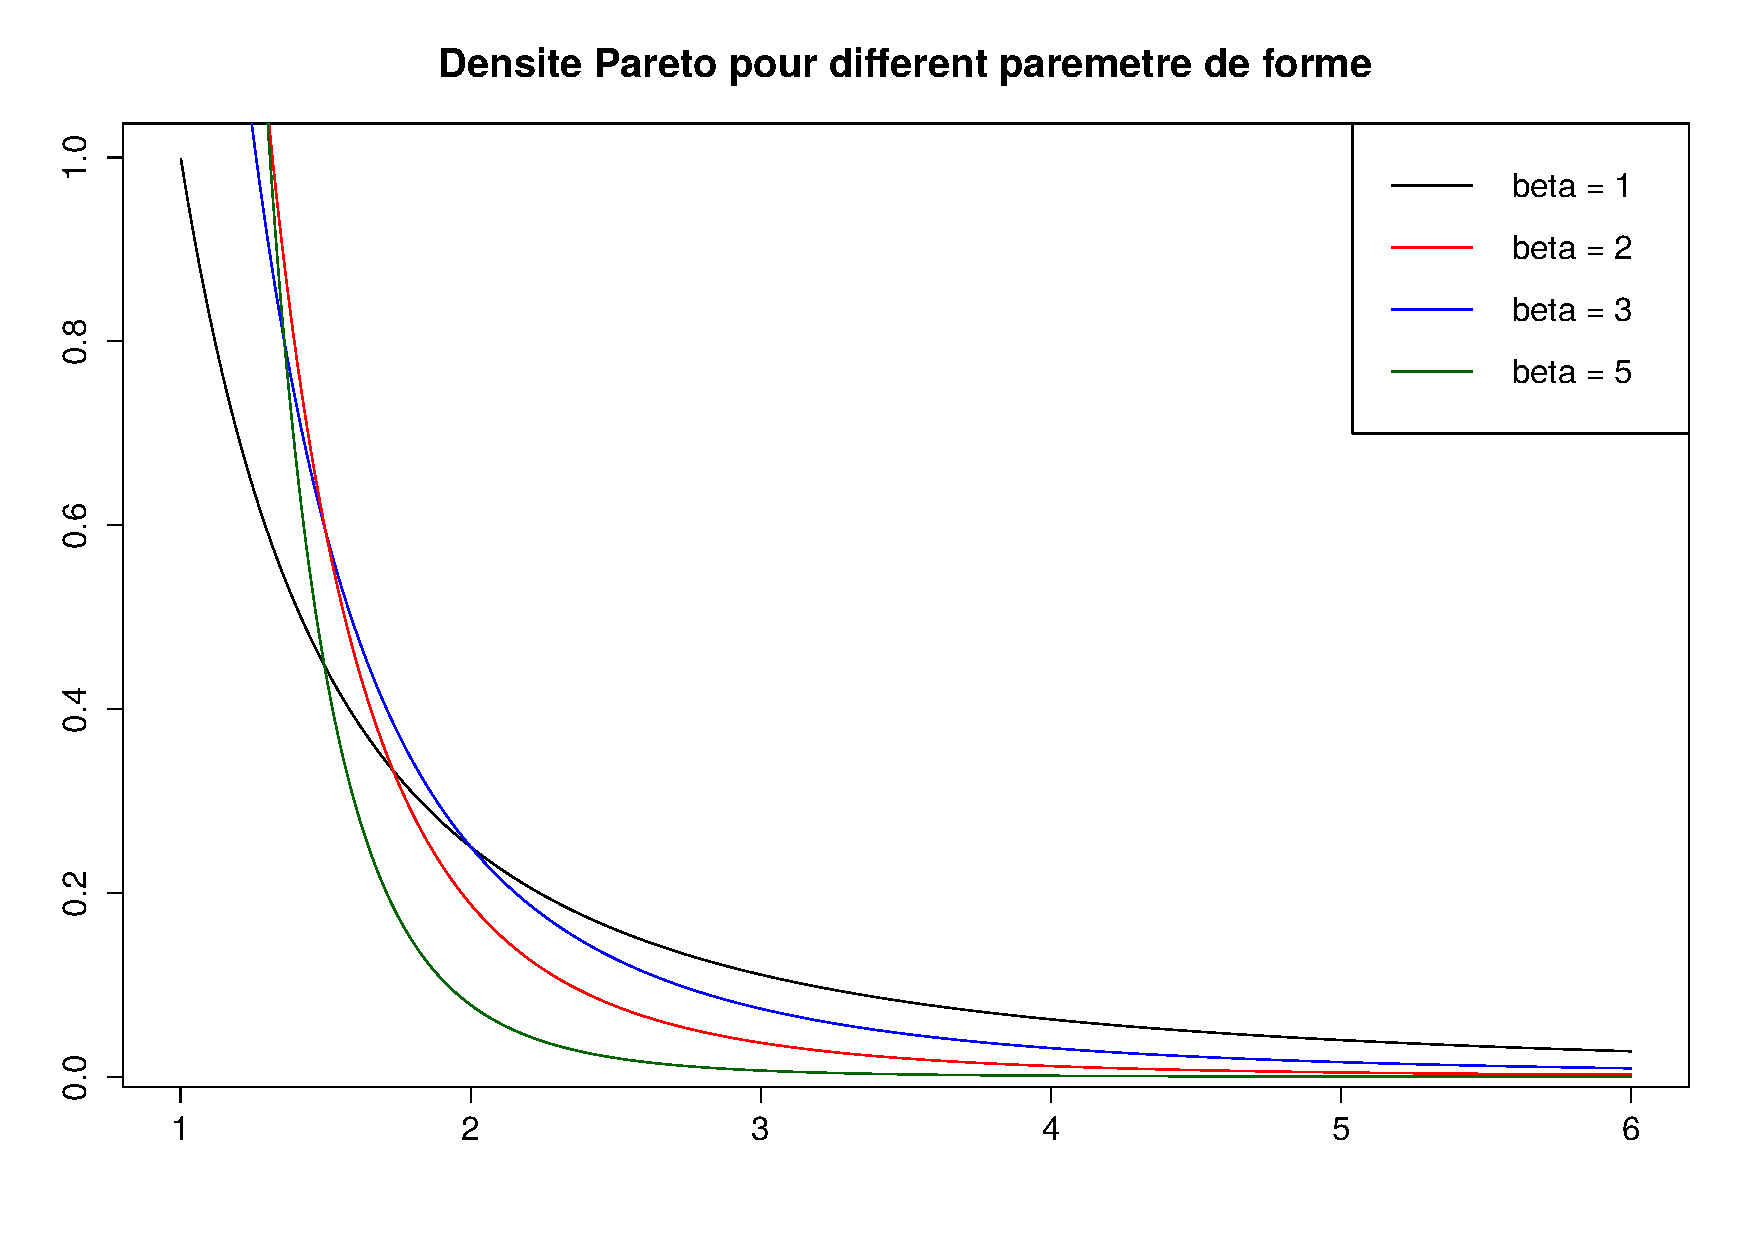
\includegraphics[width = 0.5\linewidth]{img/ParetoBetaV2}  
    \caption{Forme de la densité de la loi de Pareto pour $c=1$ et différents paramètres de forme.}
    \label{gif:Pareto}
\end{figure}

\clearpage
\section{Approche non paramétrique : l'estimateur du quantile empirique}

\subsection{Théorie et propriétés asymptotiques}
Dans cette section, on étudie l'estimateur du quantile empirique d'ordre $q$, soit  $\hat{Q_n}(q)=\hat{F_n}^{-1}(q)$, où $\hat{F_n}$ est la fonction de répartition empirique.\\
La fonction d'influence du quantile d'ordre $q$ vaut \cite{Bertail}:
\[ \label{influenceQ} T^{(1)}[x,P] = \frac{q-\mathbf{1}_{x \leq F^{-1}(q)} }{ f(F^{-1}(q)) } \]

Par le théorème de Von Mises, cet estimateur est convergent et asymptotiquement normal selon (oracle 1) 
\[ \label{var1}
\sqrt{n}[\hat{F_n}^{-1}(q)-F^{-1}(q)]\sim \emph{N} \left( 0,\frac{q(1-q)}{[f(F^{-1}(q))]^2} \right)
\]

On peut ainsi construire un intervalle de confiance asymptotique autour de la valeur de $\hat{Q_n}(q)$, soit $[\hat{Q_n}(q) \pm \frac{a_{\alpha}\sqrt{q(1-q)}}{f(\hat{Q_n}(q))\sqrt{n}}]$, où $a_{\alpha}$ est le quantile d'ordre $1-\alpha/2$ de la loi $\emph{N}(0,1)$. \\

Sans connaître la densité $f$, la variance asymptotique est inconnue. Un intervalle peut être calculé empiriquement pour l'échantillon $(X_1, ..., X_n)$. Si on considère l'échantillon ordonné $(X_{(1)}, ..., X_{(n)})$, l'intervalle $[X_{nq-\sqrt{n}a_\alpha\sqrt{q(1-q)}},X_{nq+\sqrt{n}a_\alpha\sqrt{q(1-q)}}]$, constitue un intervalle de confiance de niveau asymptotique $\alpha$.Il nécessite toutefois que le nombre d'observation $n$ soit suffisamment grand pour être correctement défini (la démonstration est fournie en annexe).\\

La vitesse de convergence est donc de l'ordre de $O(\sqrt{n})$.
Toutefois, plus l'ordre du quantile est élevé, plus la variance asymptotique est grande : le numérateur est plus élevé et le dénominateur plus faible (car on se situe dans la queue de distribution, dans laquelle la densité $f$ est plus faible). Par ailleurs, le coefficient de \textit{skewness} de cette loi très asymétrique (lorsqu'il existe !) perturbe fortement les conclusions de l'approche par l'asymptotique.\\


Le calcul des quantiles d'une telle loi peut être utilisé comme un indicateur de risque. En particulier, on peut vouloir tester si le quantile de la loi est supérieur à une valeur fixée $R$, dans le cadre d'un test de niveau $\alpha$.\\
\begin{center}
$H_0 : Q(q) \leq R$\\
$H_1 : Q(q) > R$\\
\end{center}
Le test de Wald unilatéral correspond a pour région critique :  \\

\[\frac{n(\hat{Q_n}(q)-R)^2}{\dfrac{q(1-q)}{[f(F^{-1}(q))]^2}} \geq \chi^2_{1-\alpha}\]

Ce test de niveau $\alpha$ est consistant mais on rencontre toujours le problème de la variance asymptotique, qui nécessite de connaître la densité de la loi pour être calculée.

\subsection{Bootstrap}
L'approche par l'asymptotique présente de nombreux problèmes.
D'une part, la variance asymptotique est inconnue. D'autre part, les approximations peuvent être fallacieuses, surtout pour la loi de Pareto, asymétrique et à queue lourde, et les quantiles d'ordre élevé.\\

Il s'agit désormais d'étudier différentes techniques de bootstrap dans ce contexte, afin de déterminer l'approche la plus adéquate pour pallier ces problèmes. On suppose disponible un échantillon de $n$ observations $(X_1, ..., X_n)$.

\subsubsection{Bootstrap naïf : 1a}
On considère tout d'abord l'approche classique par bootstrap : on réalise $B$ tirages avec remise parmi $(X_1, ..., X_n)$ d'un échantillon de $n$ observations $(X^*_1, ..., X^*_n)$.\\

Comme la statistique du quantile est Fréchet différentiable, le théorème de Von Mises s'extrapole au cas du bootstrap, et on obtient :
\[
\sqrt{n}\left[ \hat{F_n^*}^{-1}(q)-\hat{F_n^{-1}}(q) \right] \sim \emph{N} \( 0 ~ , ~ \frac{q(1-q)}{\left[f(F^{-1}(q))\right]^2}\)
\]

Le bootstrap est donc convergent. En revanche, il n'est pas valide au second ordre. \\
D'une part, la condition de Cramer n'est pas vérifiée car la fonction de répartition empirique est par définition à support discret. On n'a donc pas $\overline{lim}_{t\rightarrow+\infty}|\mathbb{E}_{P_n}e^{itX}|<1$.\\
De plus, la fonction d'influence de la loi empirique n'existe pas, son dénominateur étant impossible à connaître dans le cas discret.\\

L'approche par bootstrap naïf est donc convergente, mais elle est pire que l'asymptotique car elle converge seulement à une vitesse en $O(n^{1/4})$.

\begin{figure}[H]
    \centering
    \begin{subfigure}[t]{0.3\textwidth}
        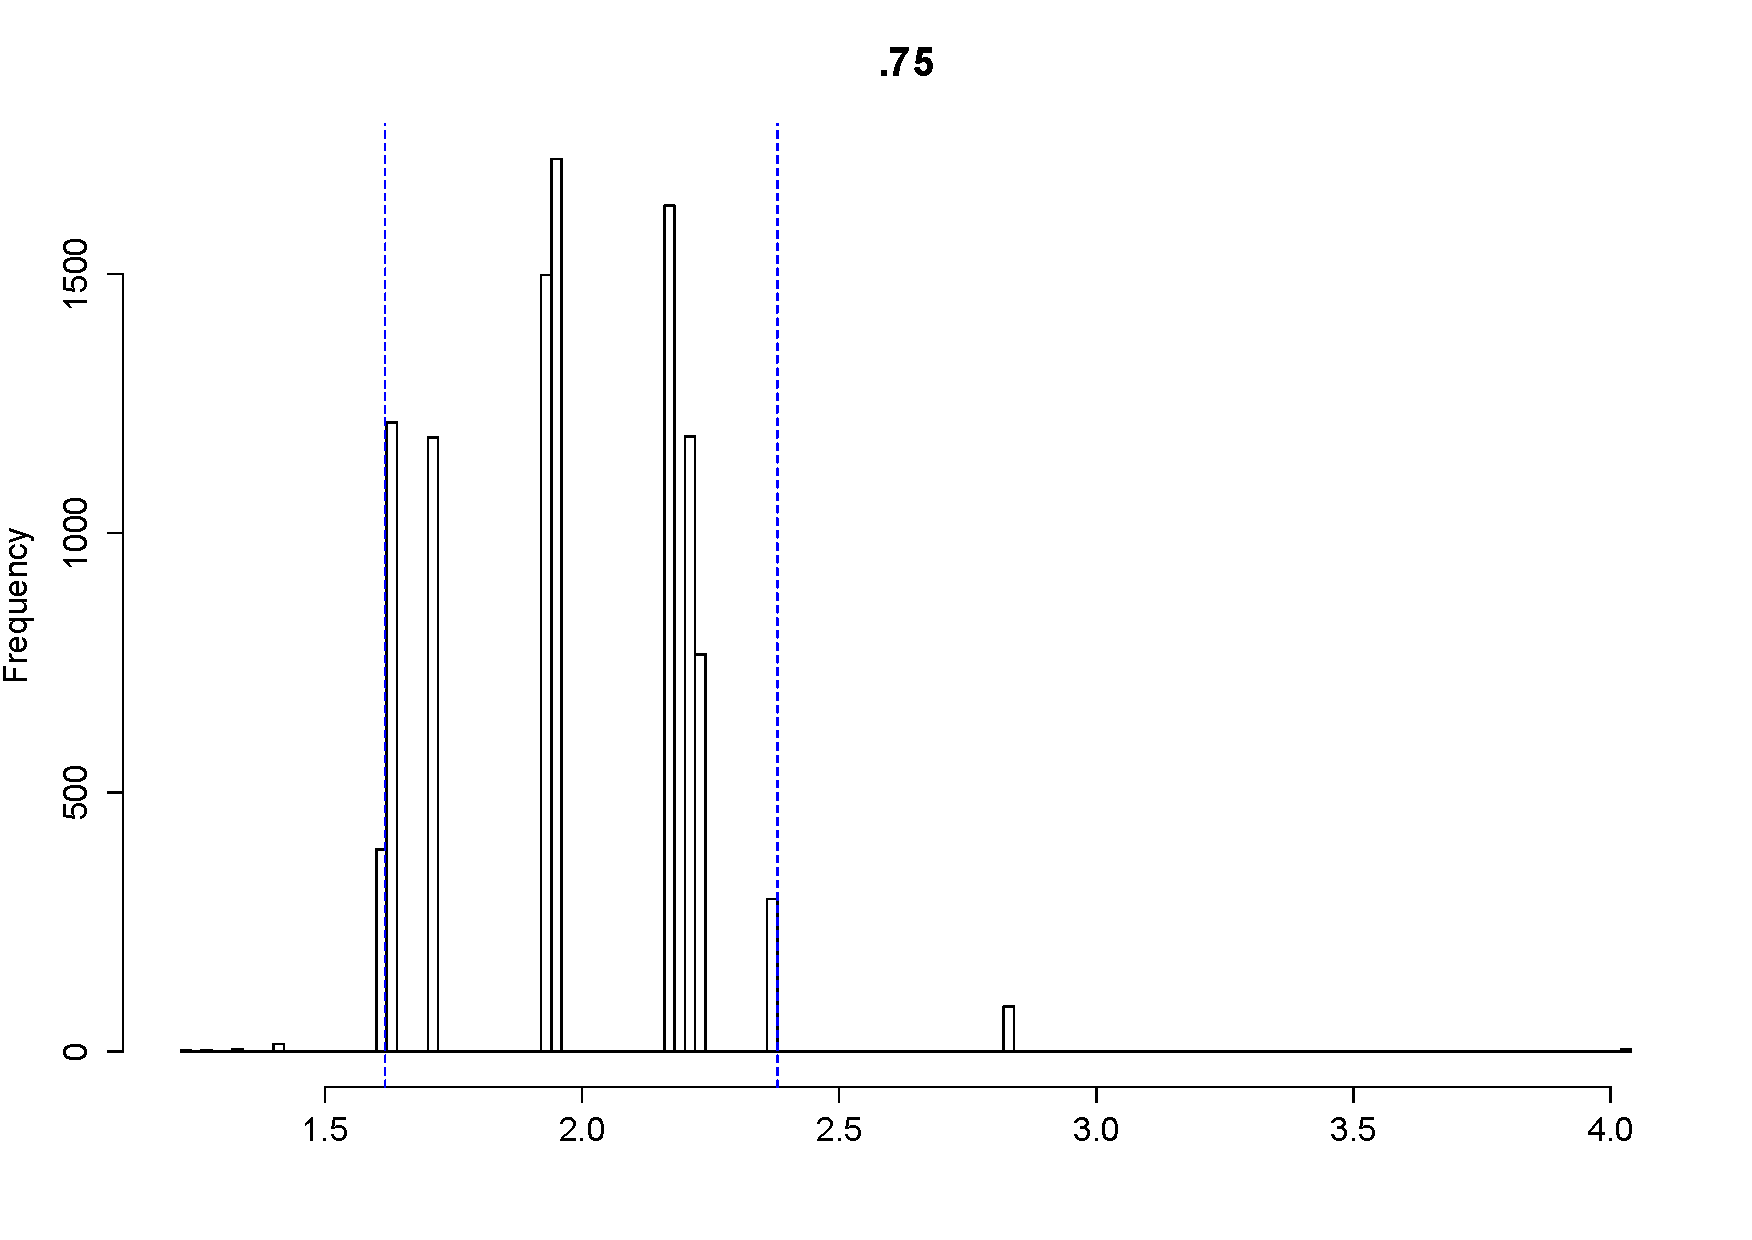
\includegraphics[width = \linewidth]{img/BootstrapNaif-75-30.pdf}
        \caption{Quantile à 75\%}
        \label{fig:naifB75}
    \end{subfigure}%
    \begin{subfigure}[t]{0.3\textwidth}
        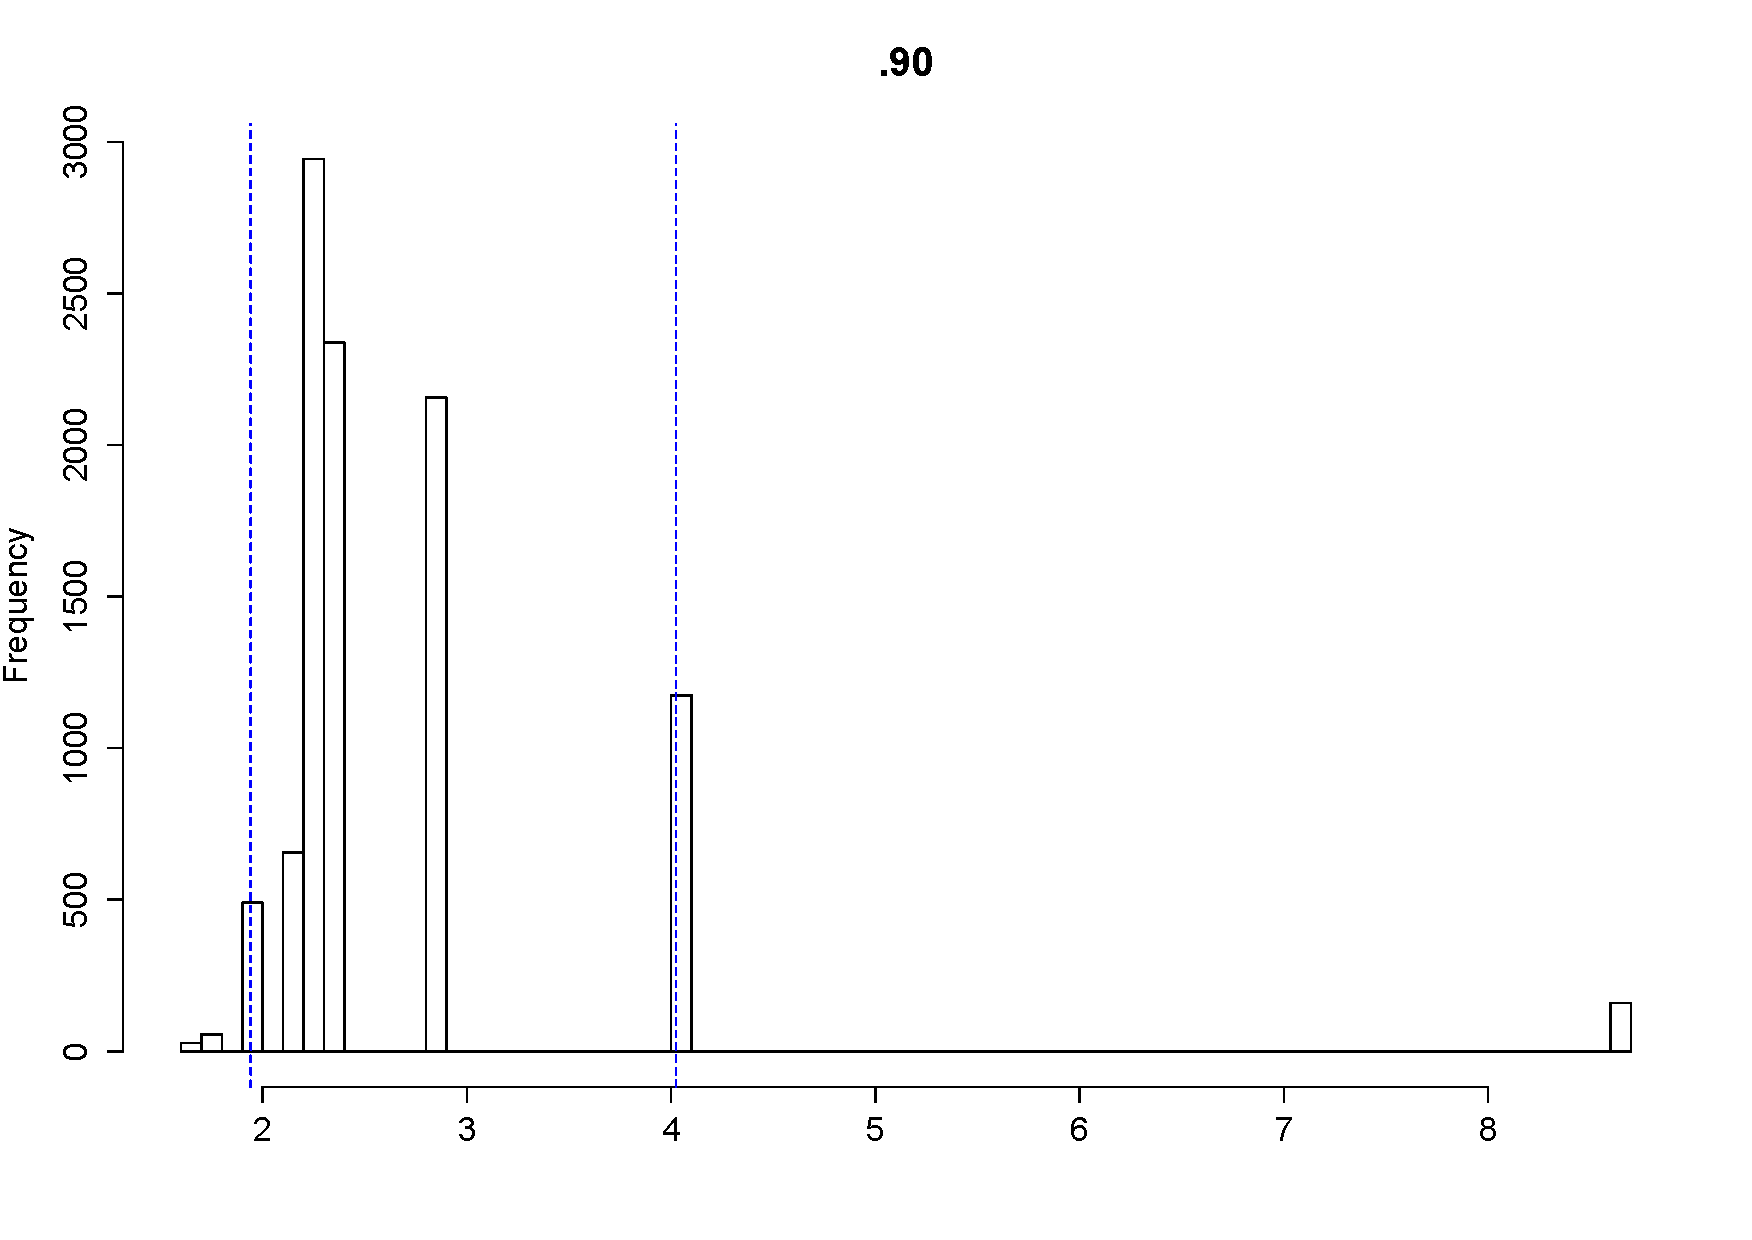
\includegraphics[width = \linewidth]{img/BootstrapNaif-90-30.pdf}
        \caption{Quantile à 90\%}
        \label{naifB90}
    \end{subfigure}%
    \begin{subfigure}[t]{0.3\textwidth}
        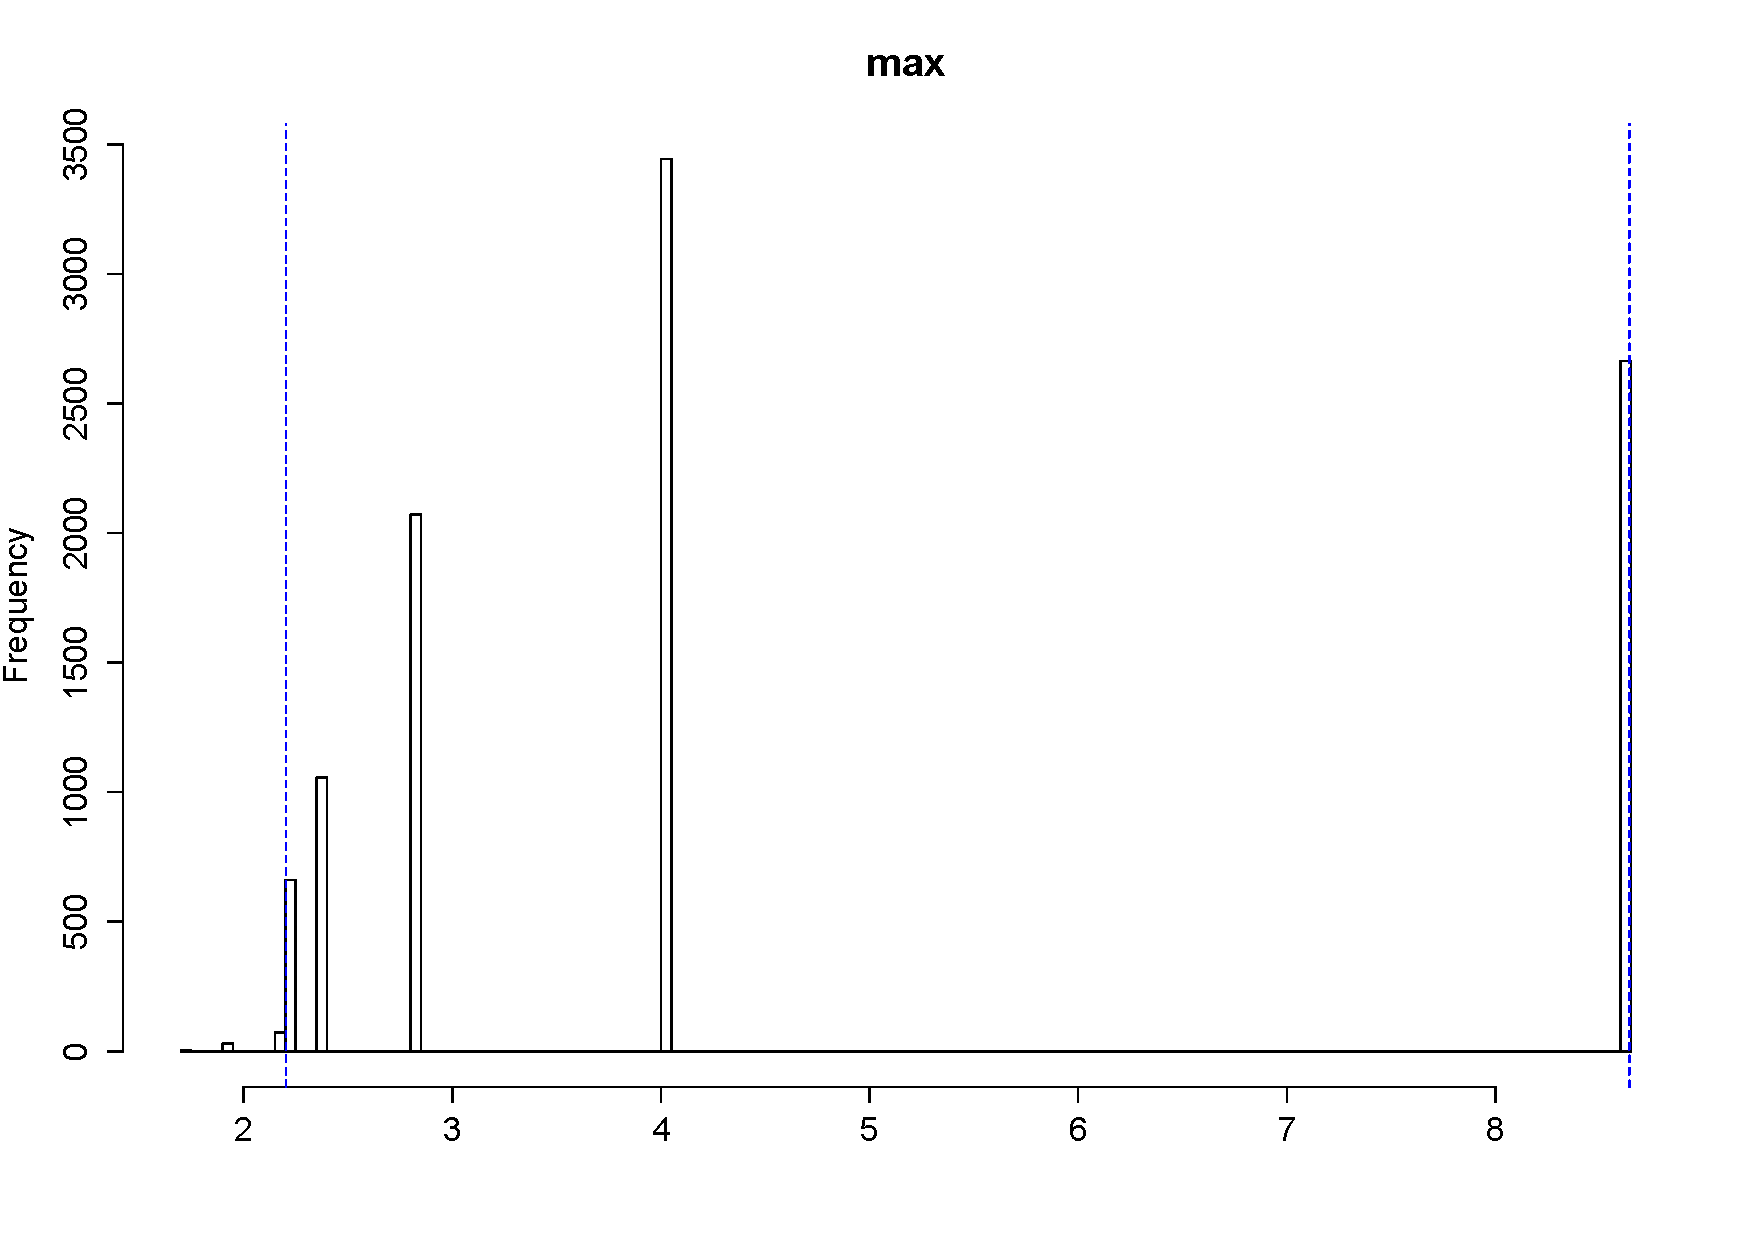
\includegraphics[width = \linewidth]{img/BootstrapNaif-Max-30.pdf}
        \caption{Quantile à 29/30}
        \label{fig:naifBMax}
    \end{subfigure}%
    \caption{Histogramme de la distribution du Bootstrap "naïf" pour n = 30. En bleu, l'intervalle de confiance à 95\%.}
    \label{fig:naifB}
\end{figure}

\begin{figure}[H]
    \centering
    \begin{subfigure}[t]{0.3\textwidth}
        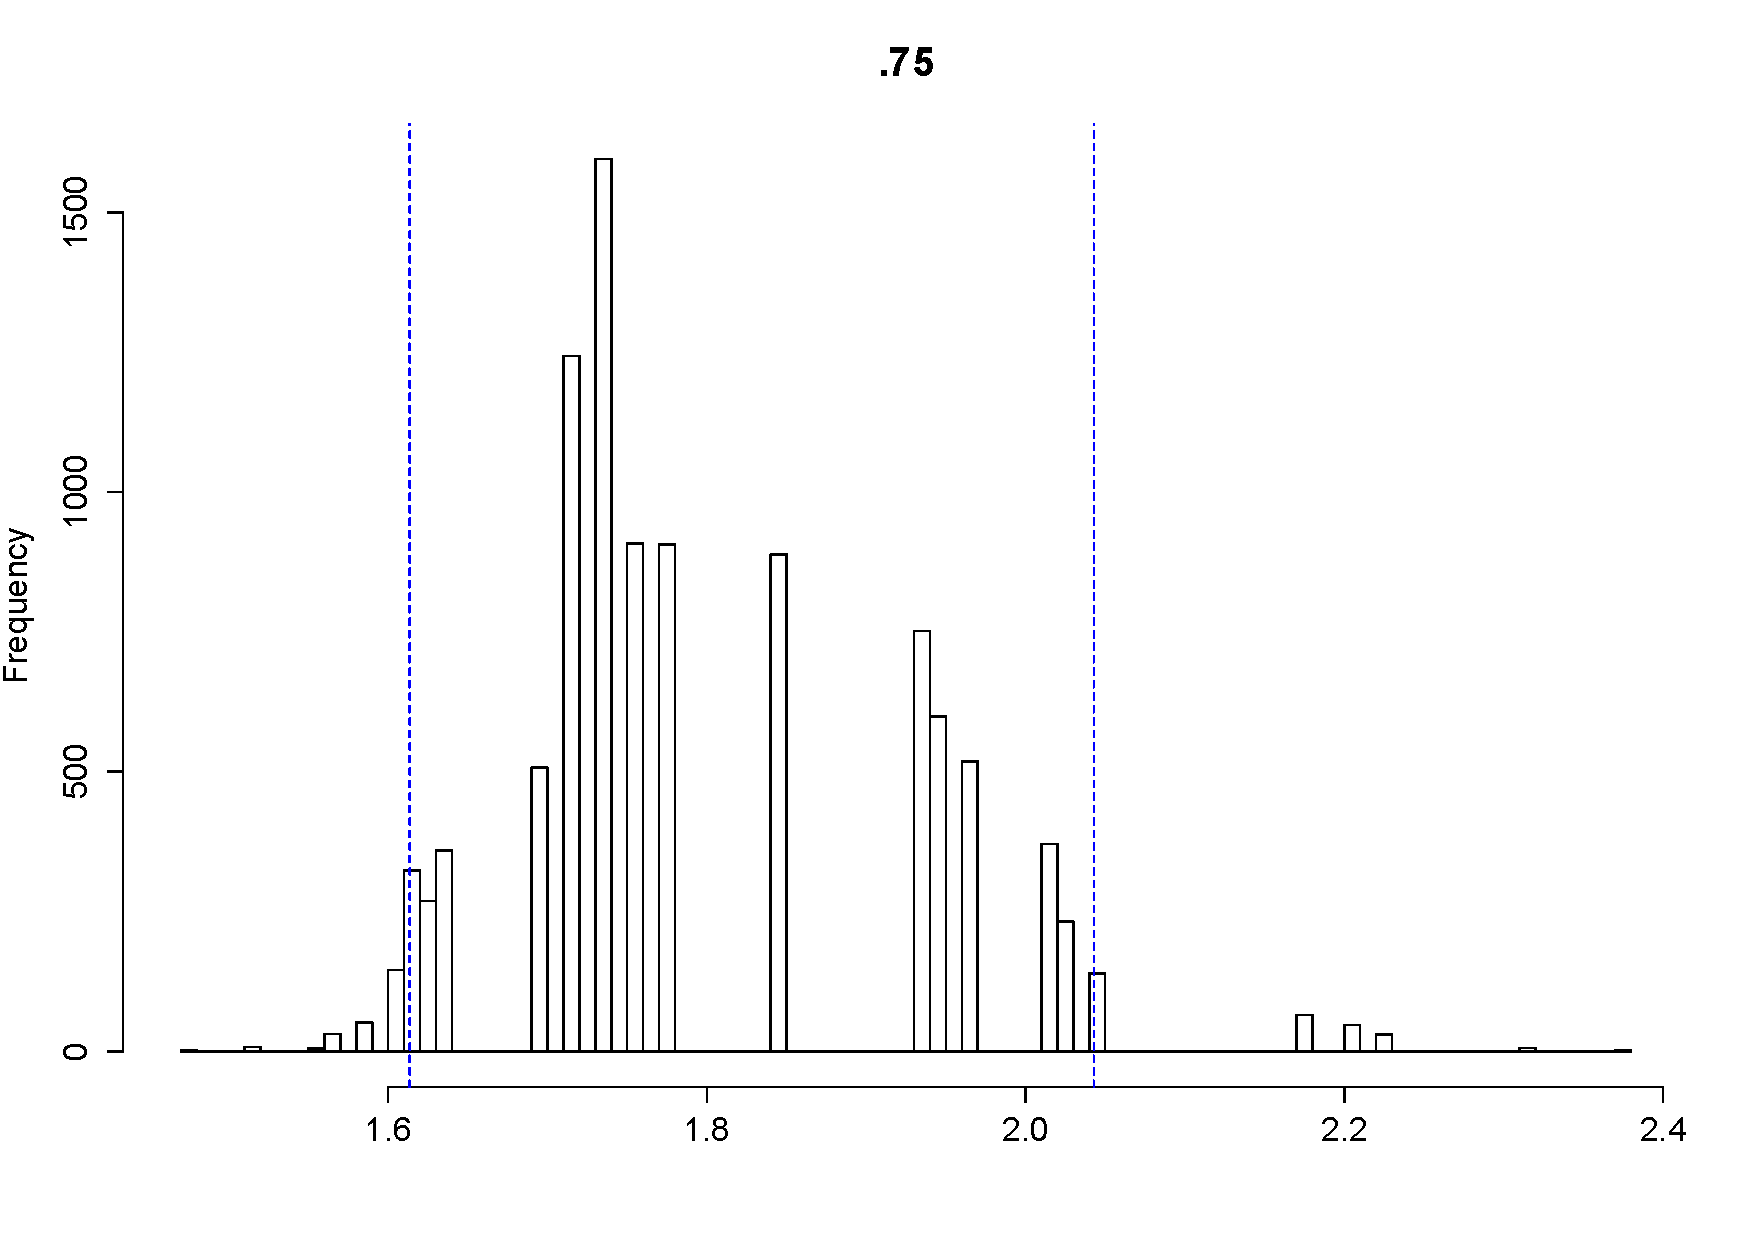
\includegraphics[width = \linewidth]{img/BootstrapNaif-75-100.pdf}
        \caption{Quantile à 75\%}
        \label{fig:naifcB75}
    \end{subfigure}%
    \begin{subfigure}[t]{0.3\textwidth}
        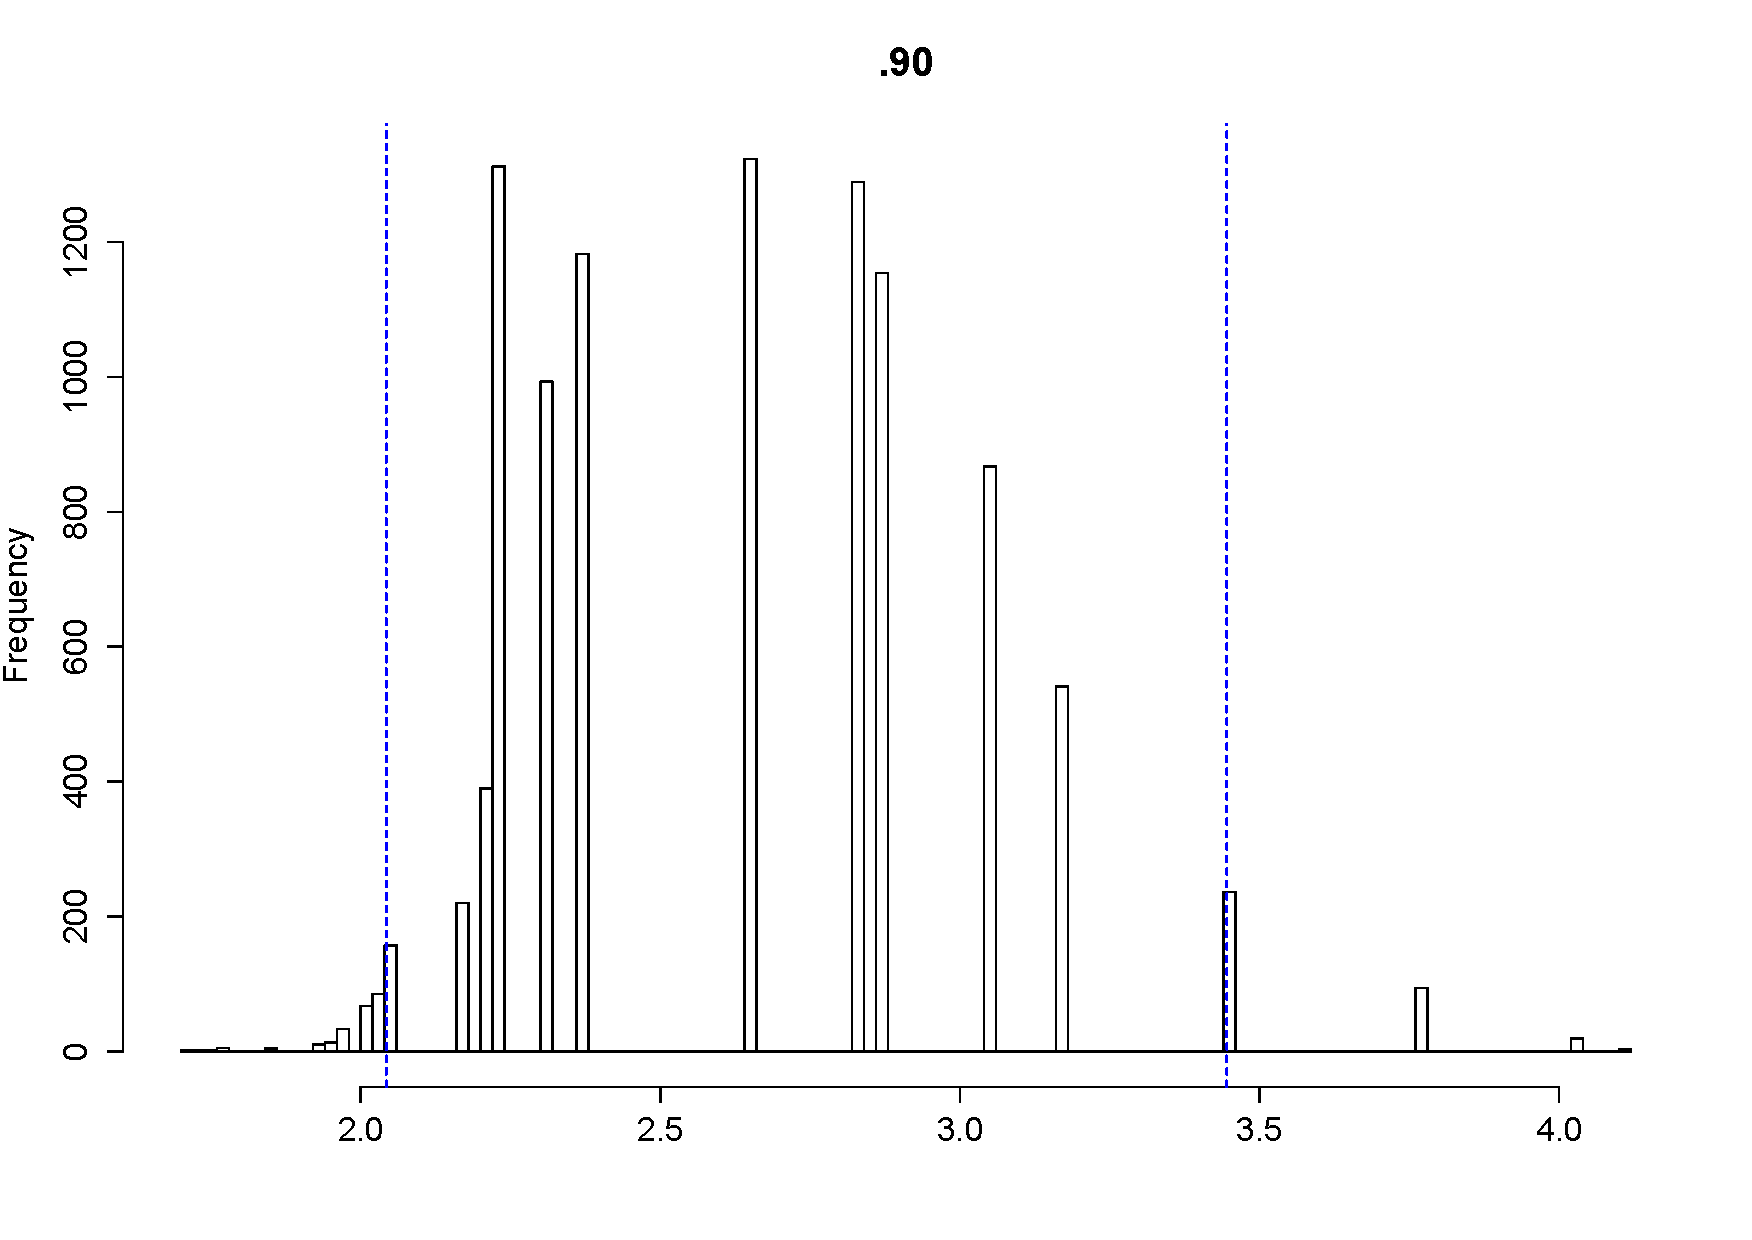
\includegraphics[width = \linewidth]{img/BootstrapNaif-90-100.pdf}
        \caption{Quantile à 90\%}
        \label{naifcB90}
    \end{subfigure}%
    \begin{subfigure}[t]{0.3\textwidth}
        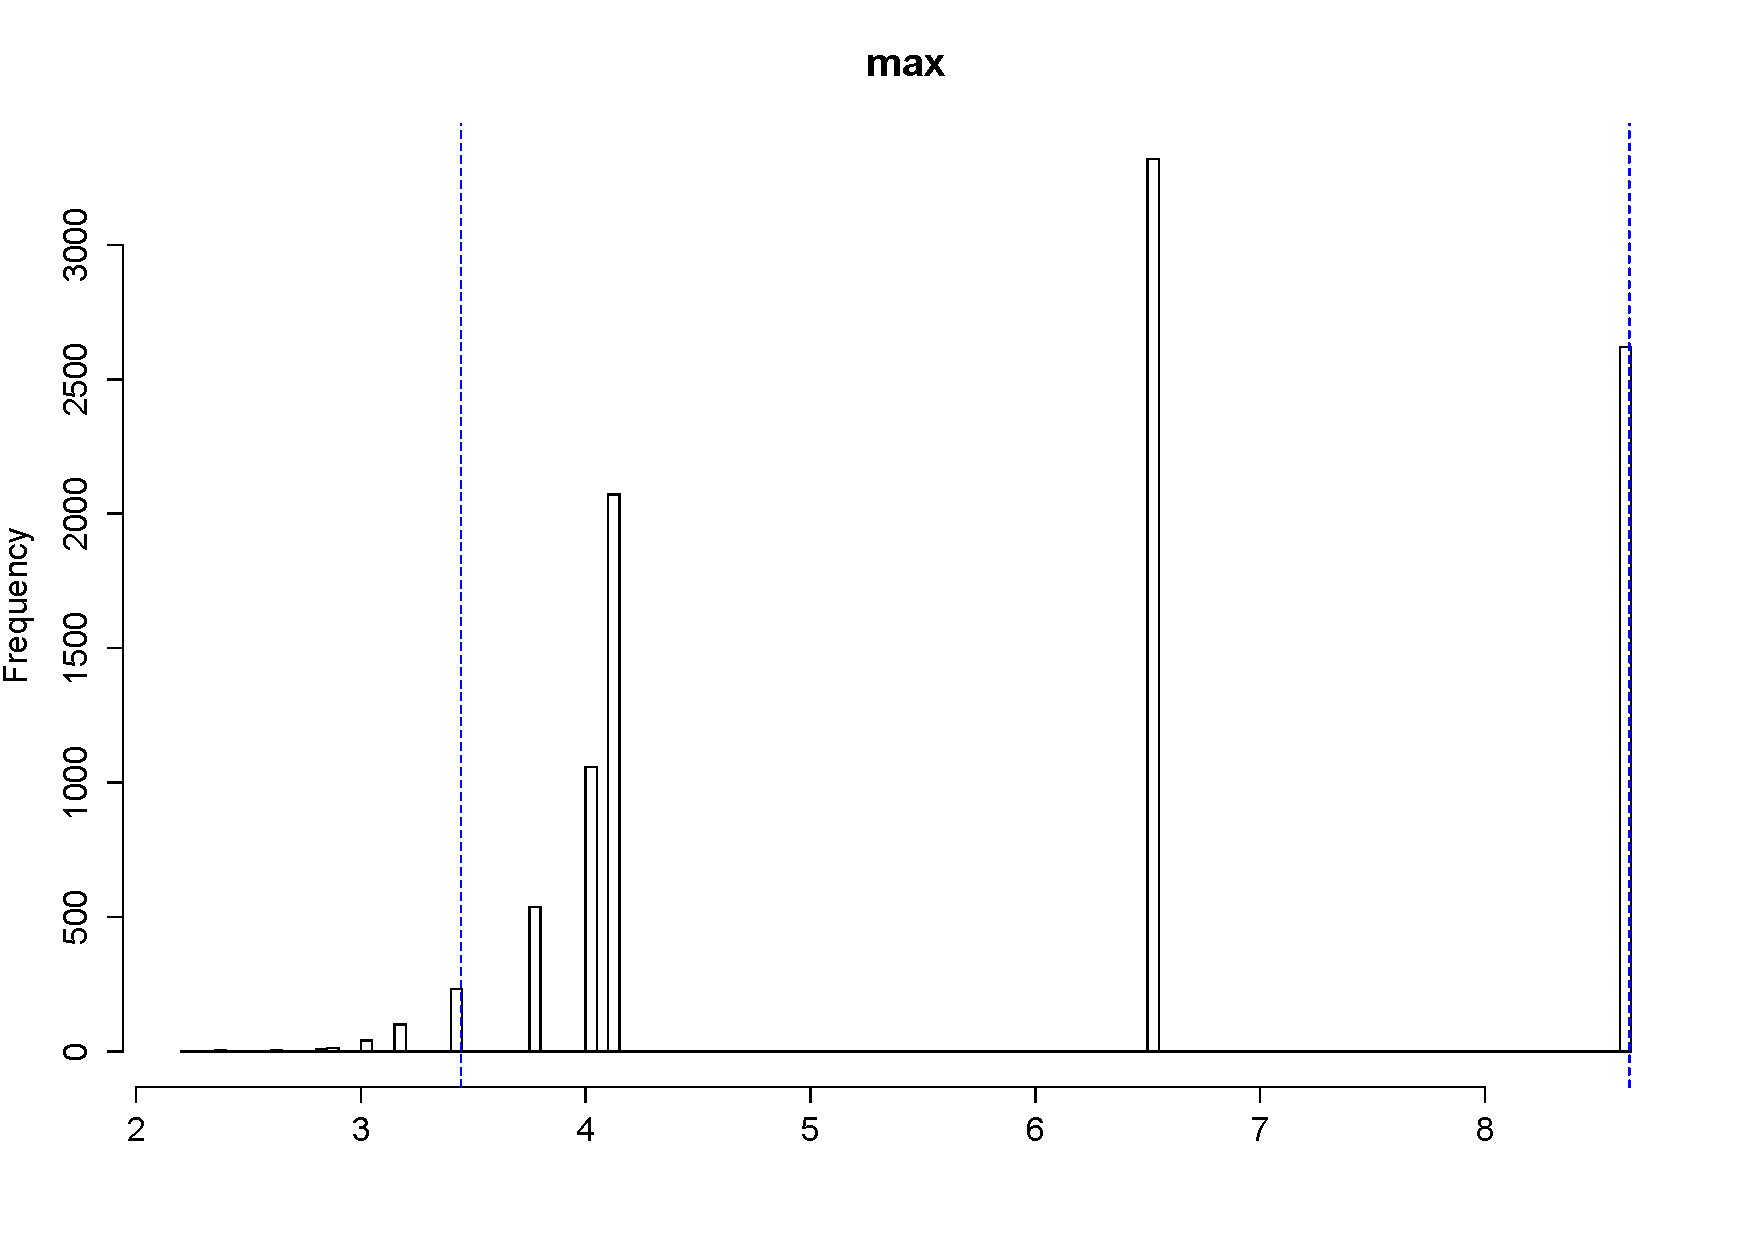
\includegraphics[width = \linewidth]{img/BootstrapNaif-Max-100.pdf}
        \caption{Quantile à 99/100}
        \label{fig:naifcBMax}
    \end{subfigure}%
    \caption{Histogramme de la distribution du Bootstrap "naïf" pour n = 100. En bleu, l'intervalle de confiance à 95\%.}
    \label{fig:naifB100}
\end{figure}

On constate graphiquement que l'estimation par bootstrap dans cette situation est bien mauvaise. Le tirage n'étant réalisé que parmi les valeurs de l'échantillon (qu'il y en ait 30 ou 100), la distribution bootstrap est concentrée sur un petit nombre de valeurs discrètes. Les estimations sont d'autant moins bonnes que l'on s'intéresse à un quantile élevé. Dans le cas du quantile maximal (1-1/n), on assiste à un échec du bootstrap qui, même au premier ordre, n'est pas convergent.

\subsubsection{Bootstrap lissé : 1b}
Afin de pallier ce défaut, on a recours au bootstrap lissé. On utilise pour cela un noyau $K_{h_n}$. On simule un $B$ échantillons $(\epsilon^{i}_1, ..., \epsilon^{i}_n)$ ($i=1...B$) selon $K_{h_n}$. Ensuite, l'échantillon boostrap $(X^*_1, ..., X^*_n)$ numéro $i$ est tiré avec remise dans $(X_1+\epsilon^{i}_1, ...,X_n+ \epsilon^{i}_n)$. Chaque échantillon bootstrap est donc tiré avec remise dans l'ensemble des observations perturbées.\\

Par exemple, dans le cas du noyau gaussien, on a $(N_1, ...,N_n) \sim \emph{N}(0,1)$, $(\tilde{X^*_1},...,\tilde{X^*_n})$ tirés indépendamment dans $\hat{F_n}$, et $X_i^* = \tilde{X^*_i}h_nN_i$, ($i=1...n$). On répète $B$ fois cette opération.\\

Le lissage de la fonction de répartition empirique permet l'existence de la fonction d'influence de la loi empirique. Ainsi, le développement d'Edgeworth peut se calculer et sous certaines hypothèses de régularité, on obtient la validité du bootstrap au second ordre. Dans le cas d'un noyau gaussien, on a ainsi une vitesse de convergence en $O(n^{-3/4})$.
% ecrire le développement d'edgeworth

Il est nécessaire de bien choisir la fenêtre $h_n$ : en particulier, il faut respecter les conditions 
$nh_n \rightarrow +\infty$ et $h_n \rightarrow 0$.\\

\begin{equation*}
Pr\left[ \sqrt{n}\frac{T(P^*_n)-T(P_n)}{S_n} \leq x\right]-Pr\left[\sqrt{n}\frac{T(P_n)-T(P)}{S_n} \leq x \right]=O\(n^{-3/4}\)
\end{equation*}


\begin{figure}[H]
    \centering
    \begin{subfigure}[t]{0.3\textwidth}
        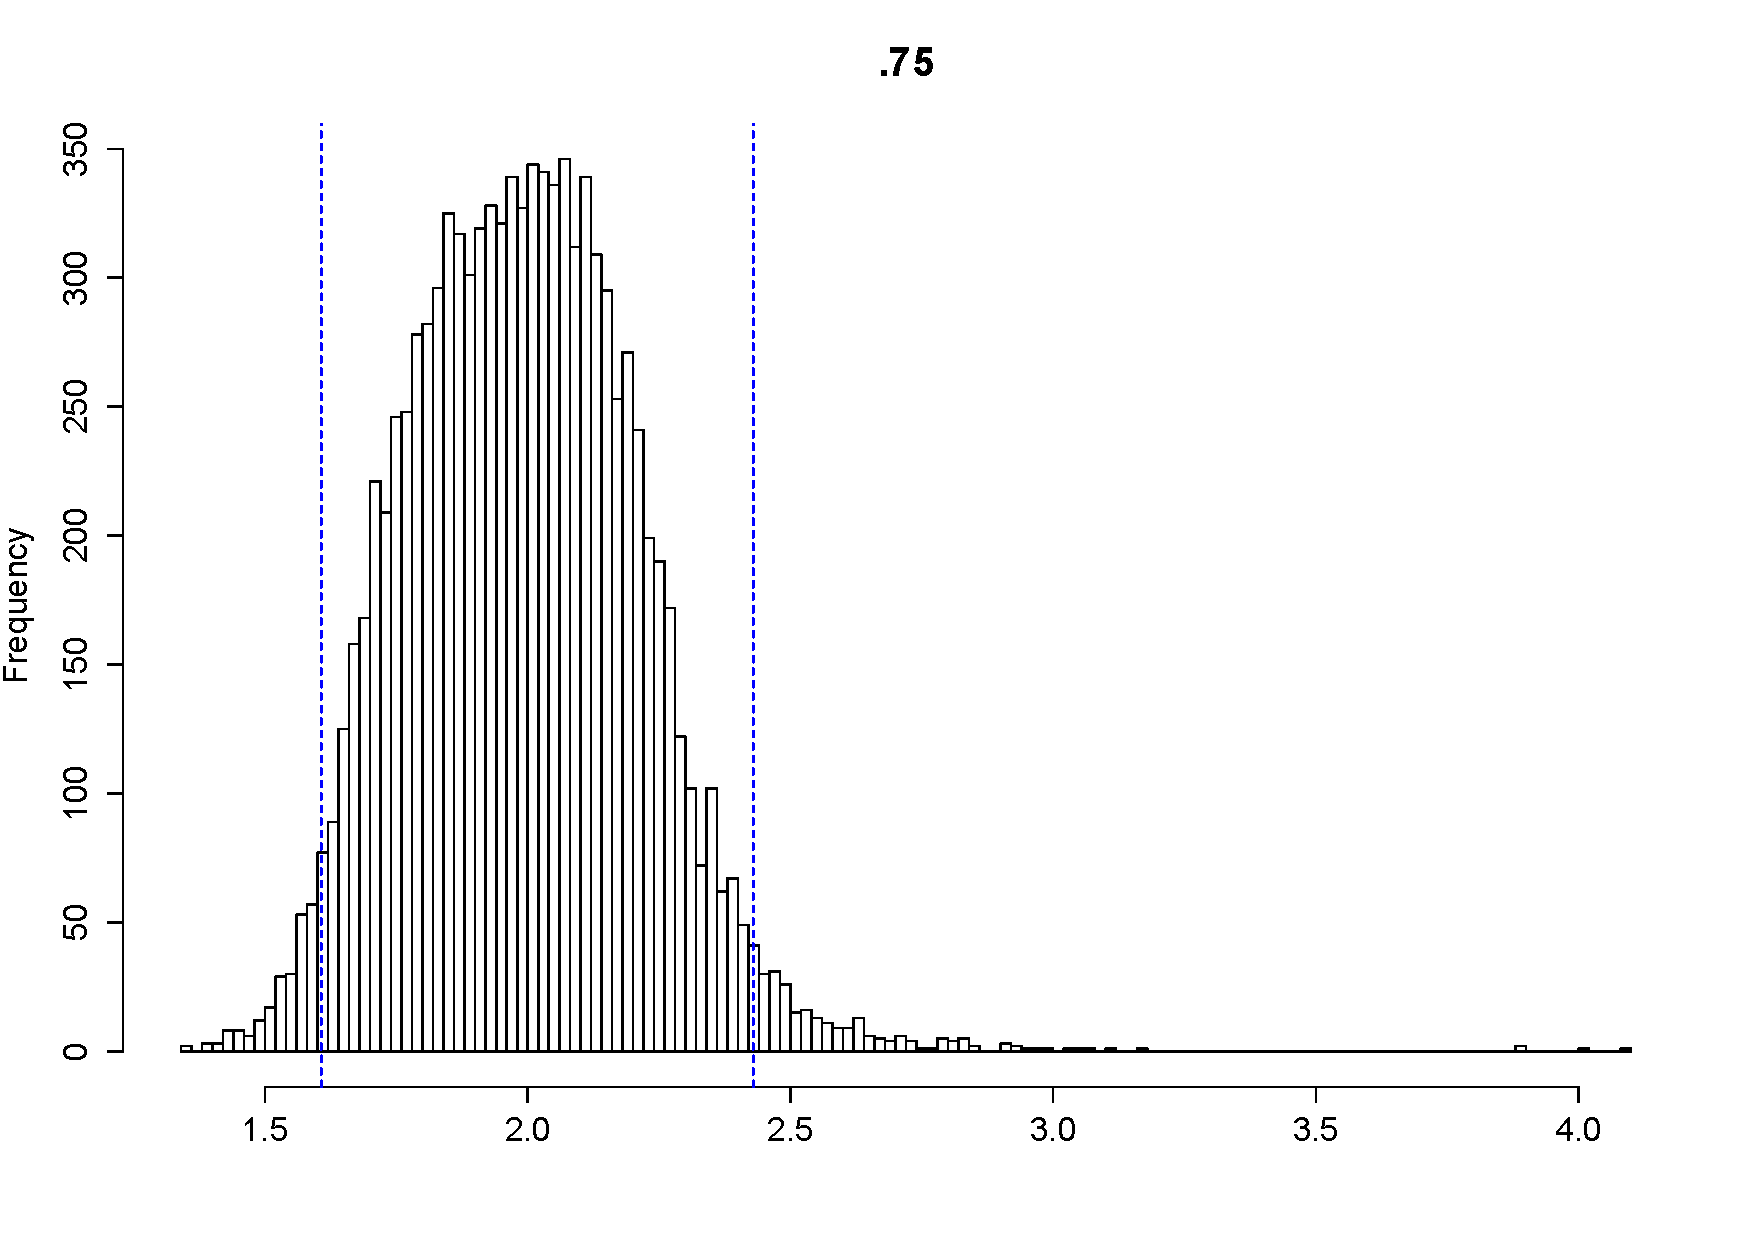
\includegraphics[width = \linewidth]{img/BootstrapSmooth-75-30.pdf}
        \caption{Quantile à 75\%}
        \label{fig:smooth3B75}
    \end{subfigure}%
    \begin{subfigure}[t]{0.3\textwidth}
        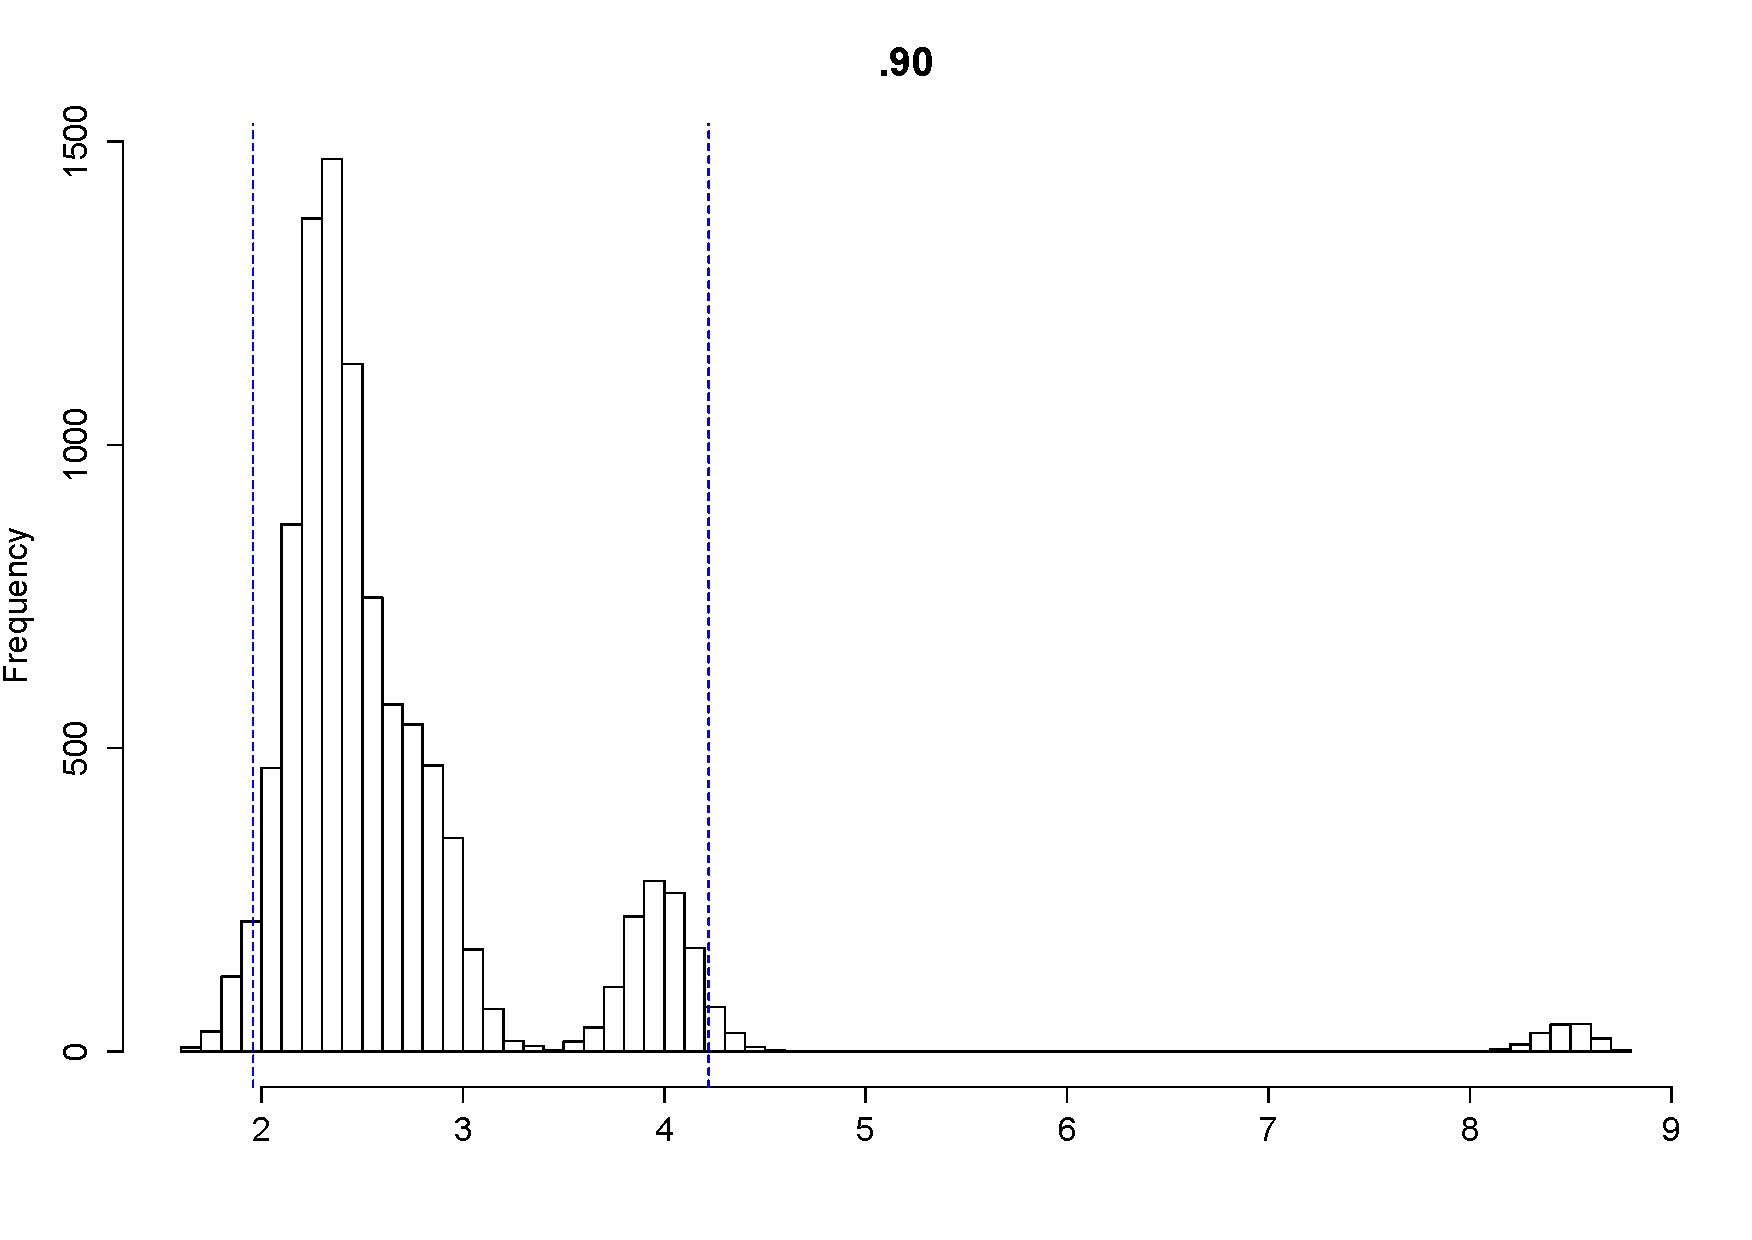
\includegraphics[width = \linewidth]{img/BootstrapSmooth-90-30.pdf}
        \caption{Quantile à 90\%}
        \label{fig:smooth390}
    \end{subfigure}%
    \begin{subfigure}[t]{0.3\textwidth}
        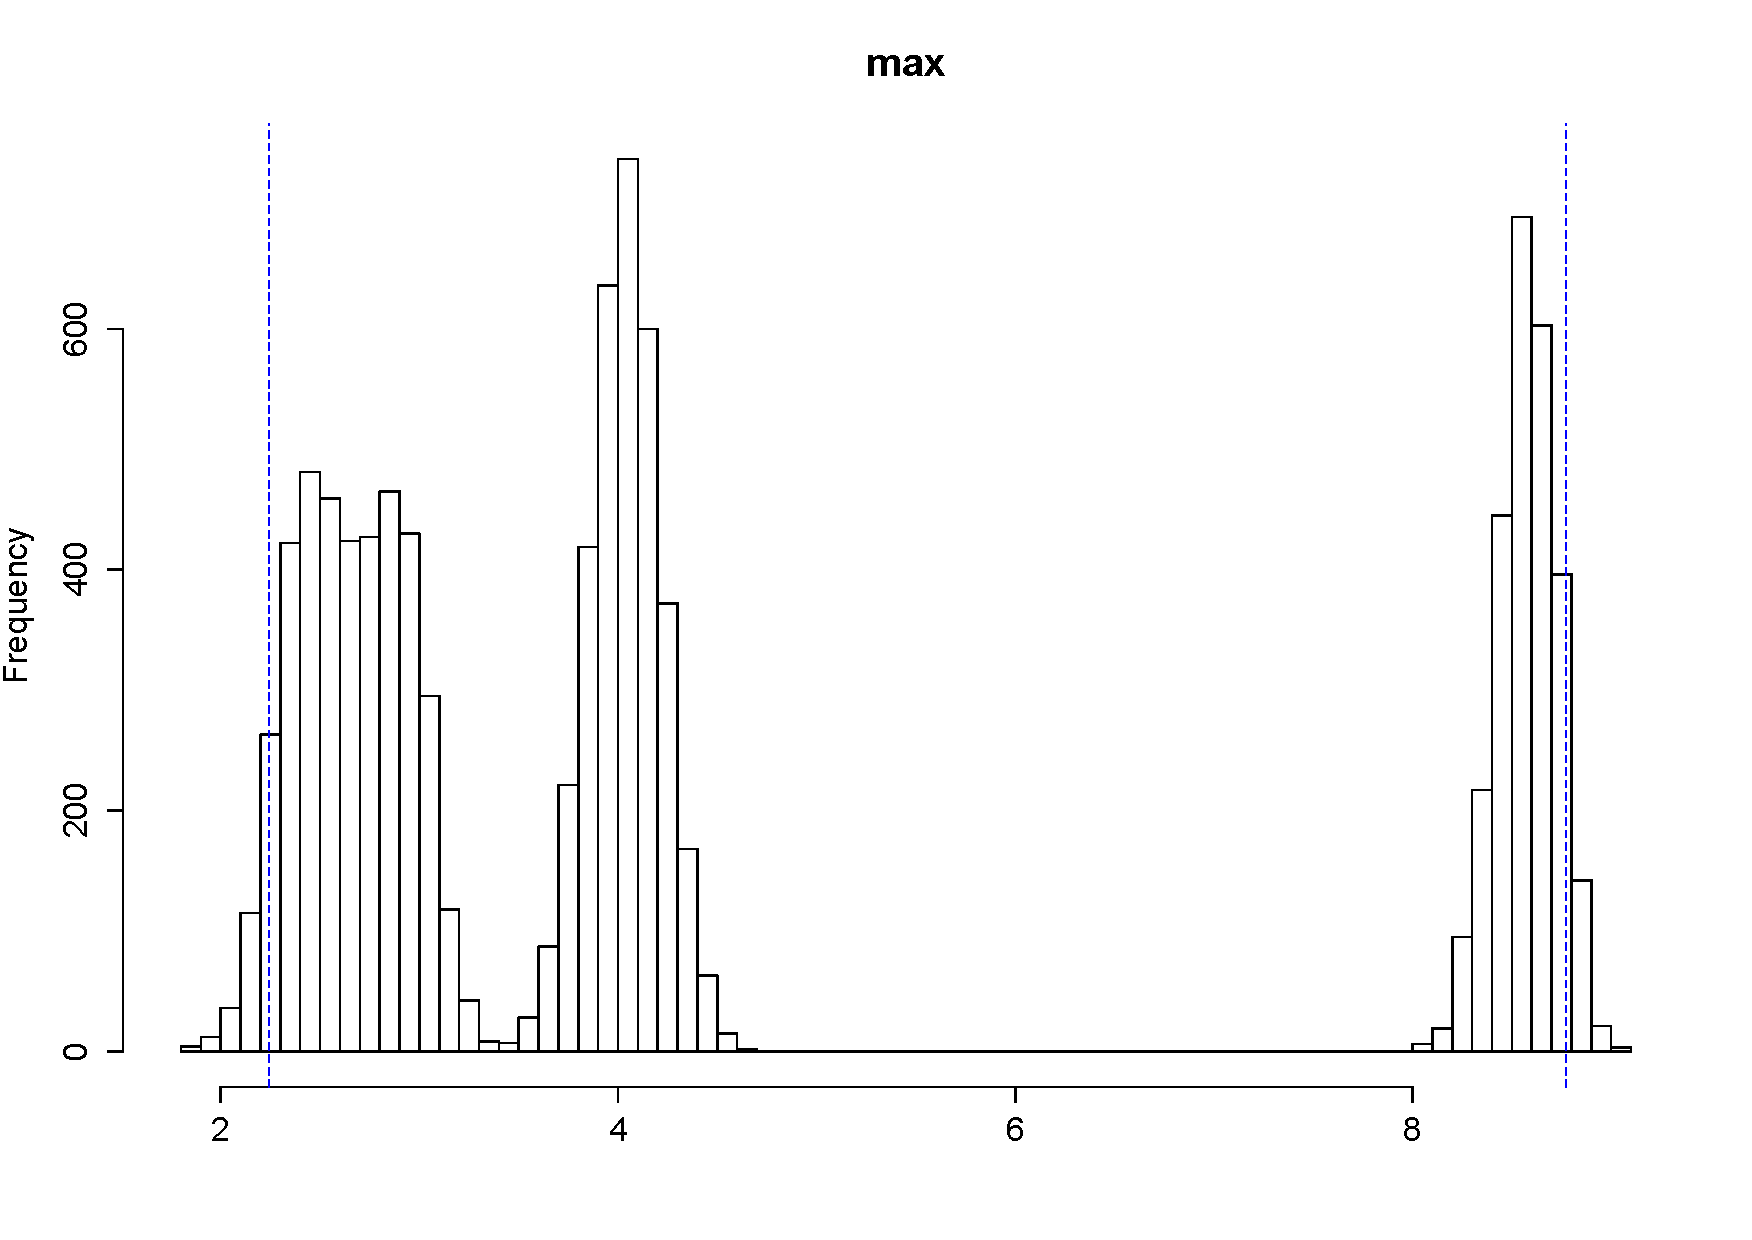
\includegraphics[width = \linewidth]{img/BootstrapSmooth-Max-30.pdf}
        \caption{Quantile à 29/30}
        \label{fig:smooth3BMax}
    \end{subfigure}%
    \caption{Histogramme de la distribution du Bootstrap "lissé" pour n = 30. En bleu, l'intervalle de confiance à 95\%. On utilise un noyau gaussien et on fixe $h_n =1/\sqrt{n}$.}
    \label{fig:smoothB30}
\end{figure}

\begin{figure}[H]
    \centering
    \begin{subfigure}[t]{0.3\textwidth}
        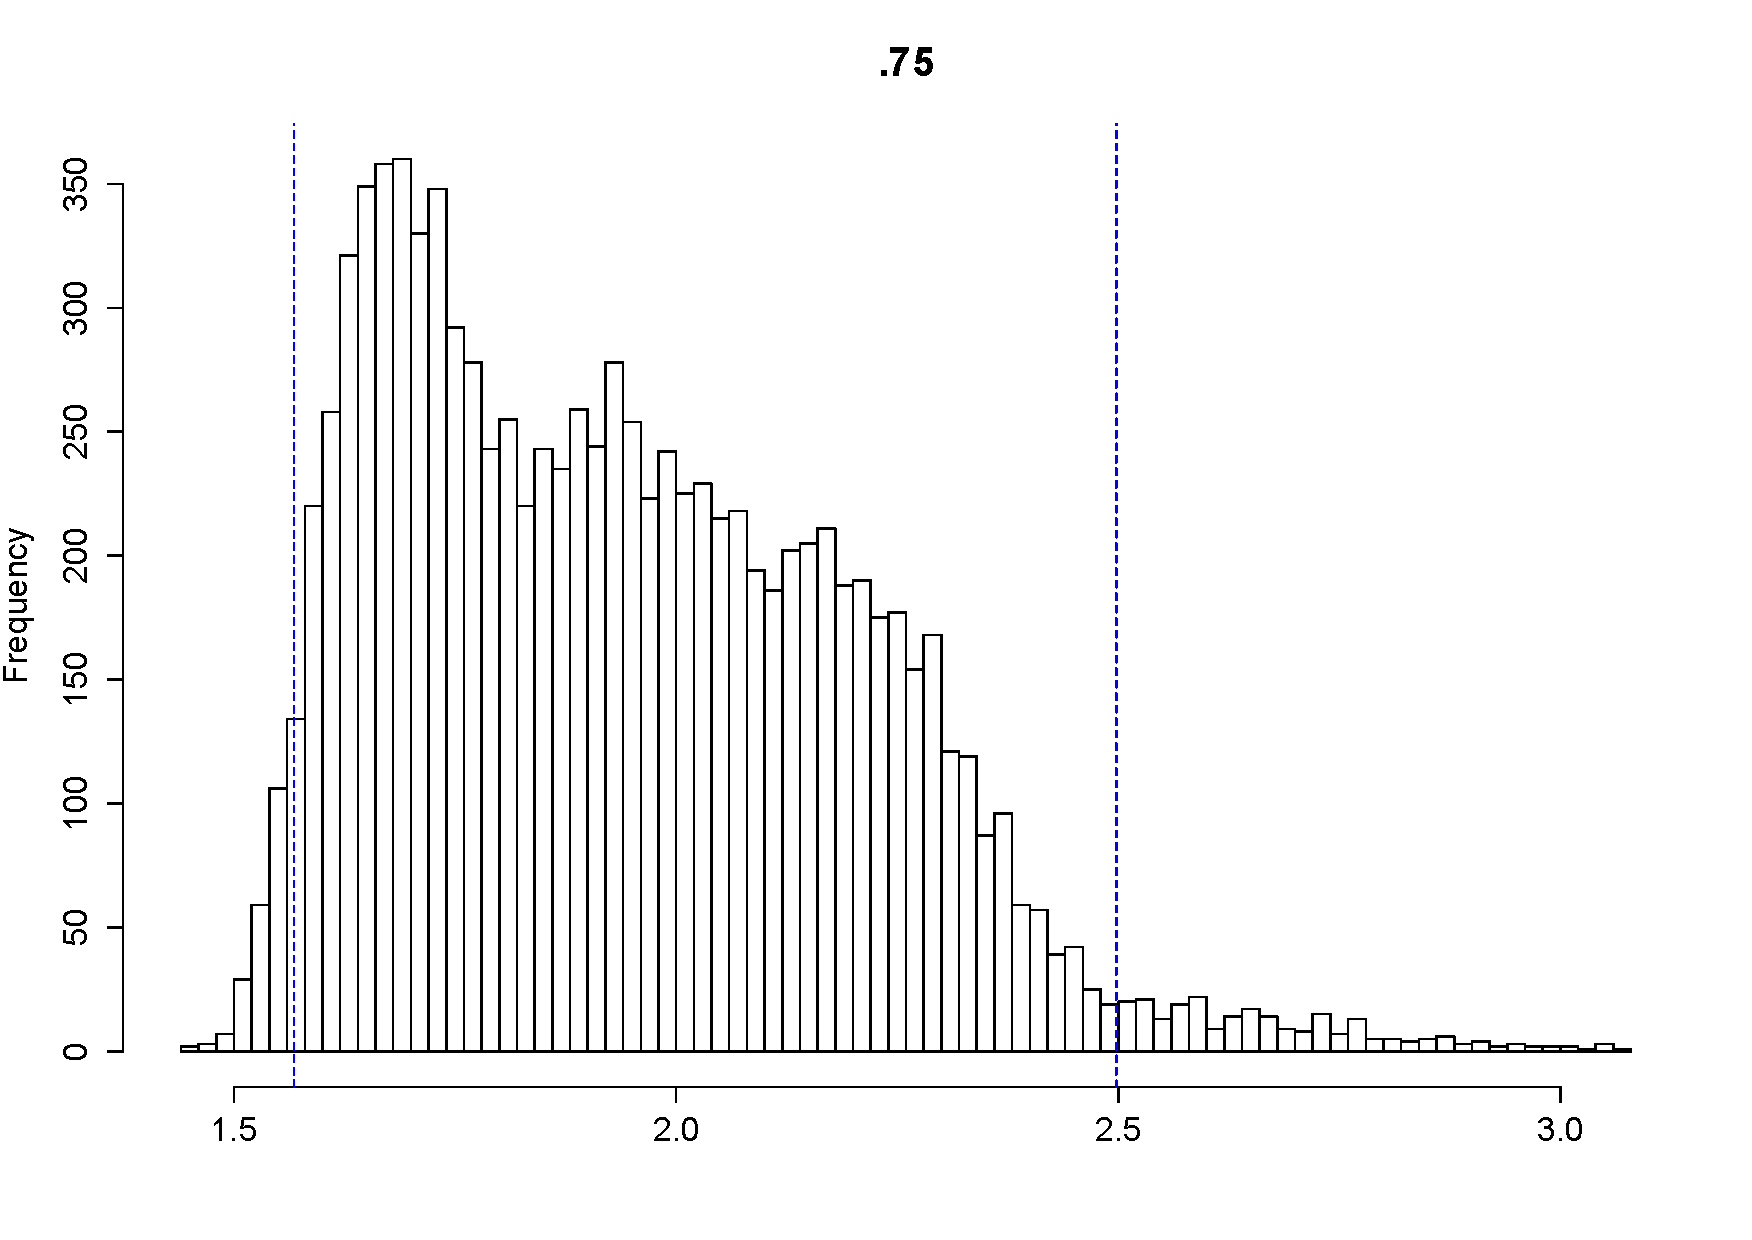
\includegraphics[width = \linewidth]{img/BootstrapSmooth-75-100.pdf}
        \caption{Quantile à 75\%}
        \label{fig:smoothB75}
    \end{subfigure}%
    \begin{subfigure}[t]{0.3\textwidth}
        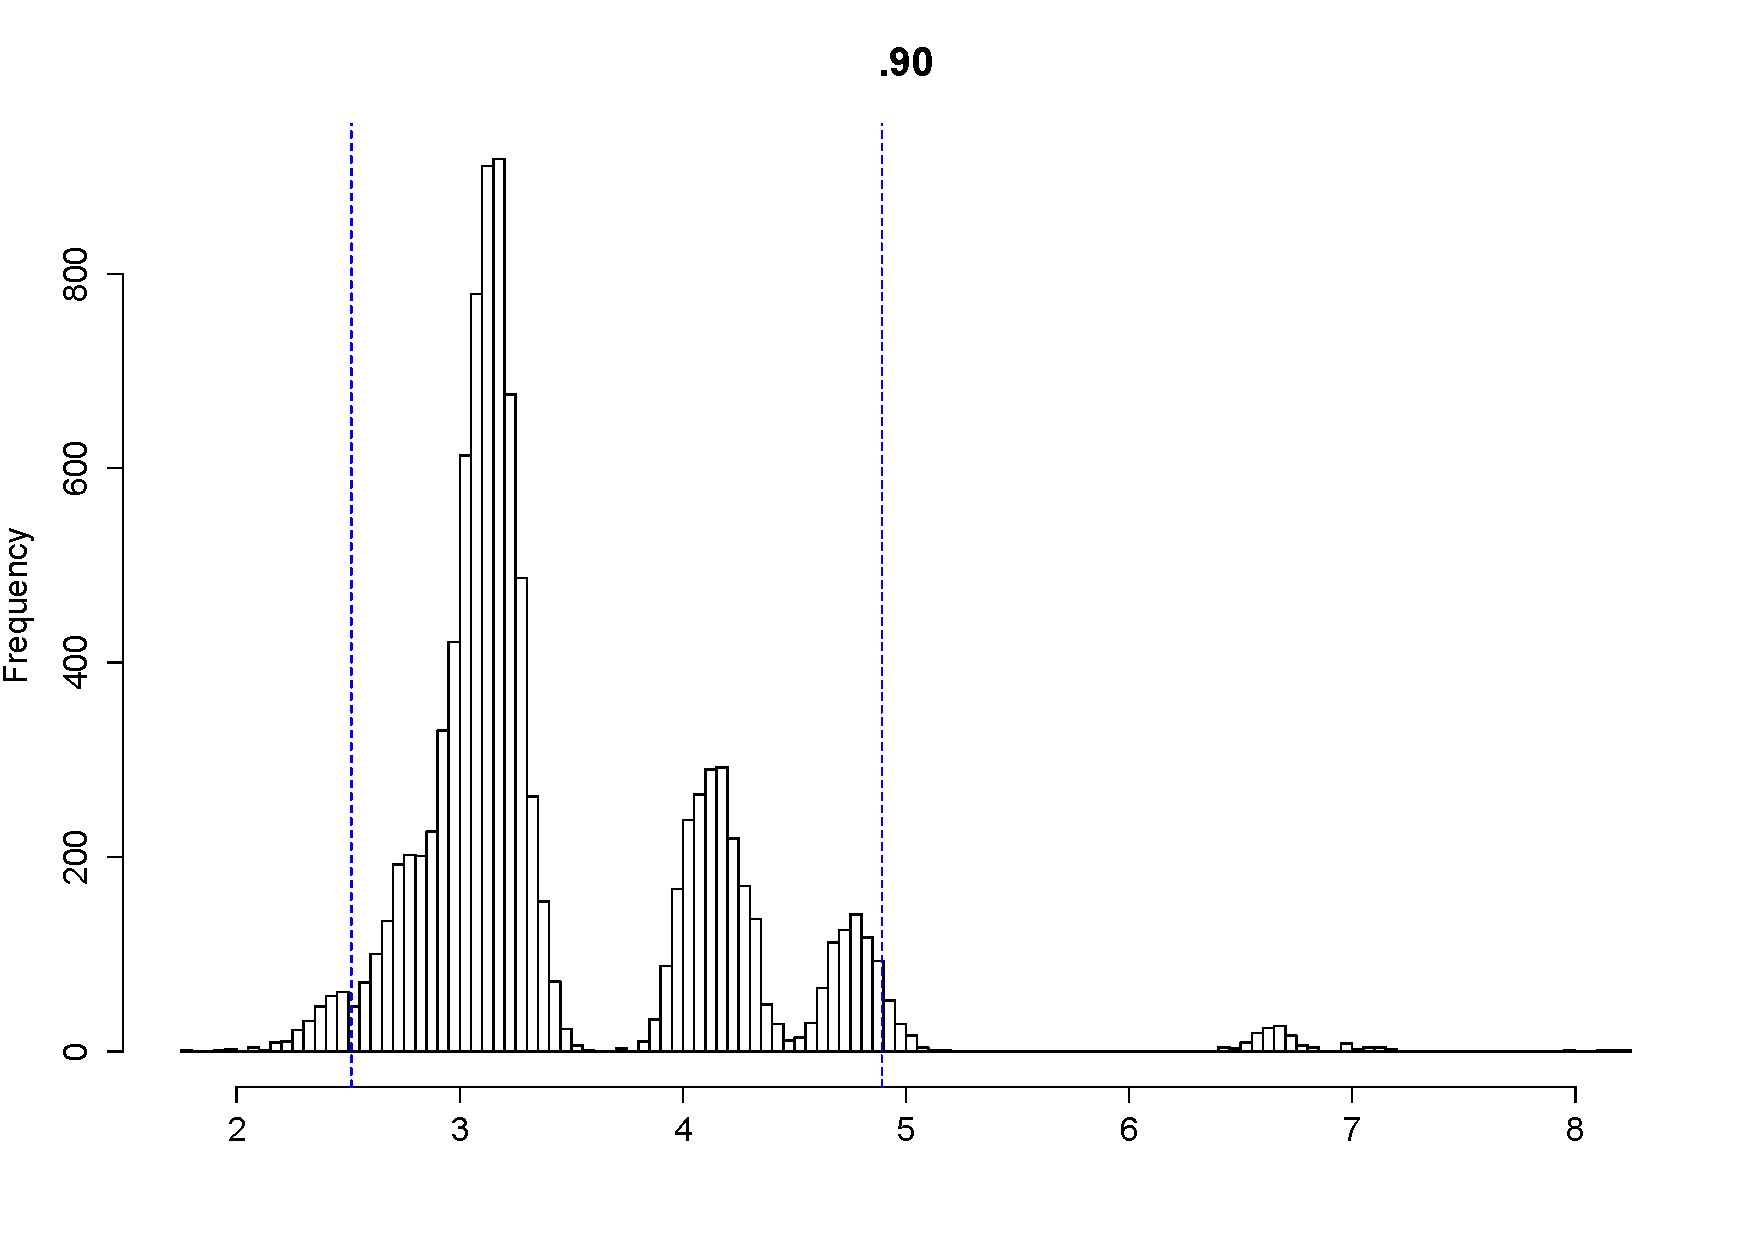
\includegraphics[width = \linewidth]{img/BootstrapSmooth-90-100.pdf}
        \caption{Quantile à 90\%}
        \label{fig:smooth90}
    \end{subfigure}%
    \begin{subfigure}[t]{0.3\textwidth}
        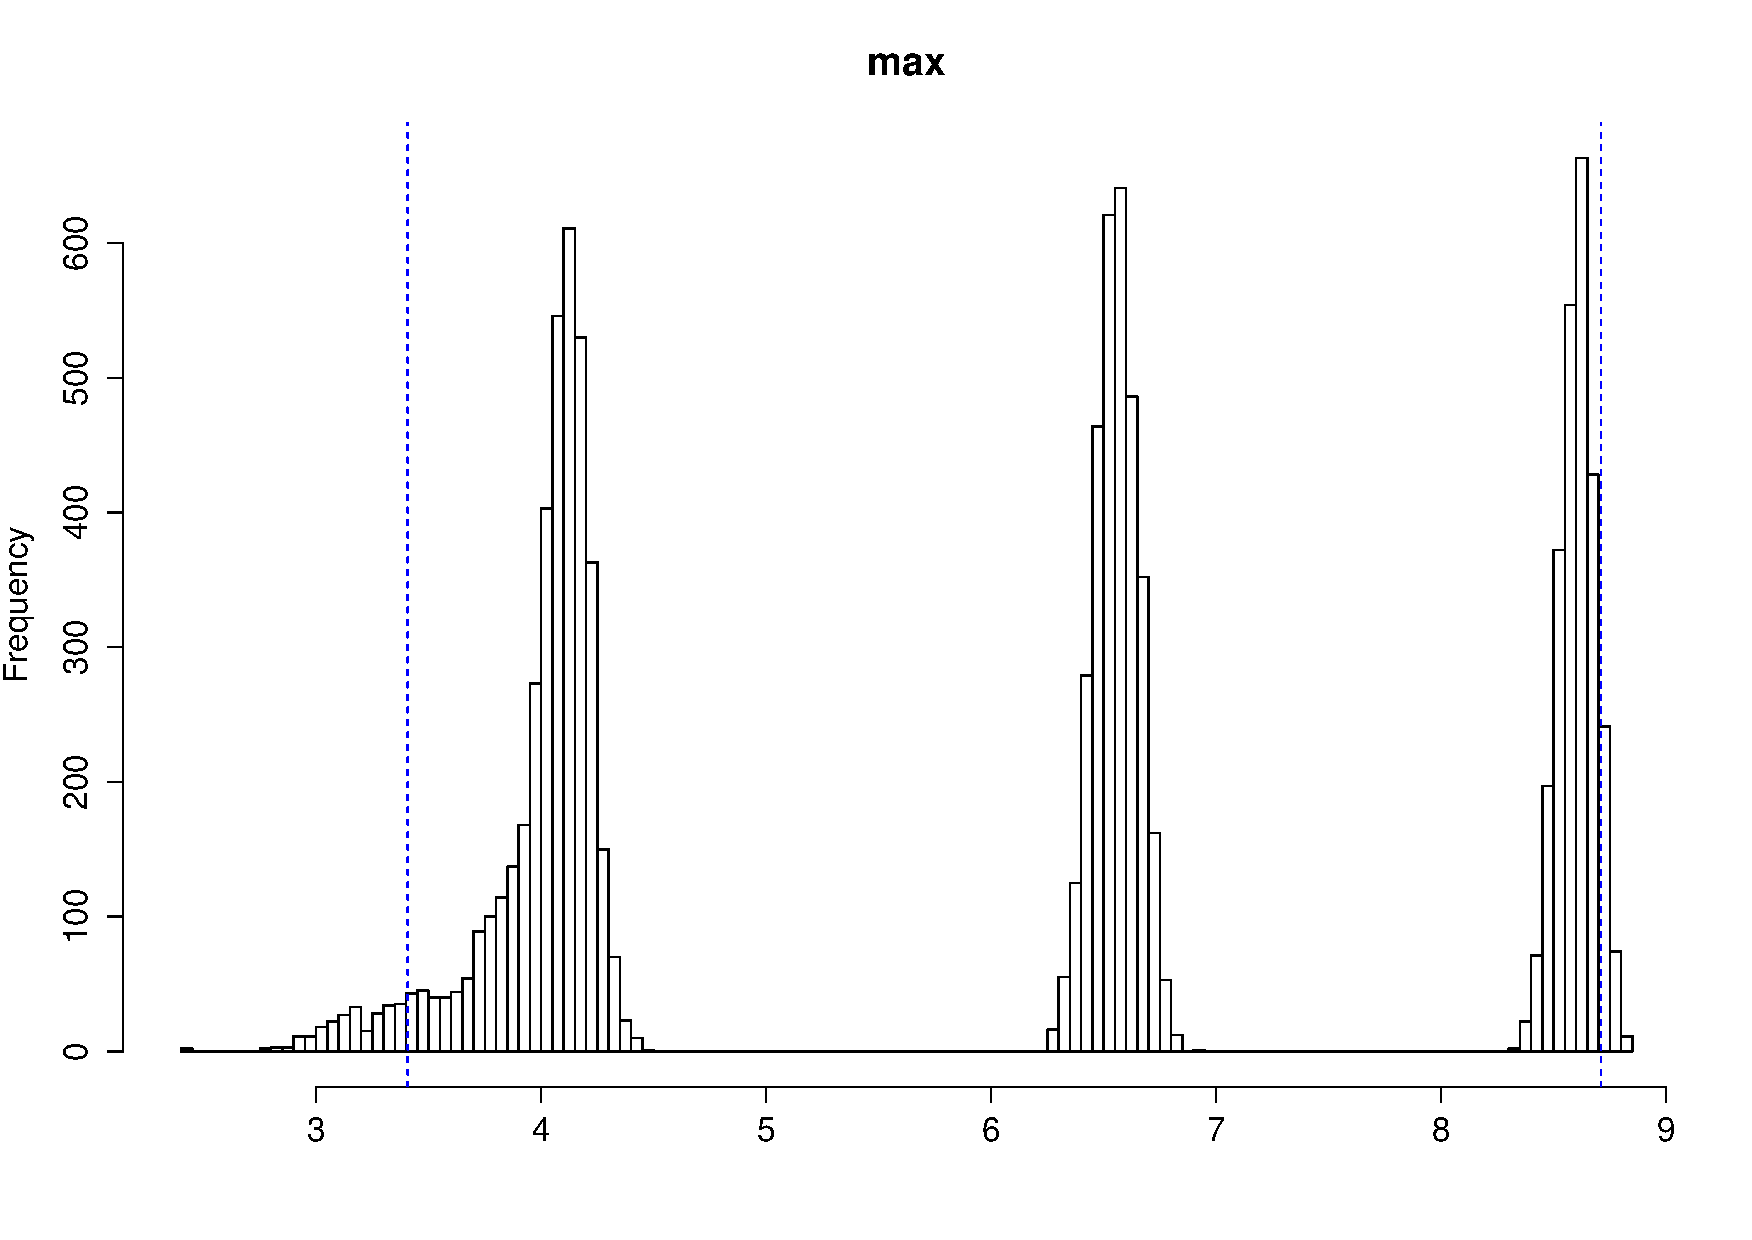
\includegraphics[width = \linewidth]{img/BootstrapSmooth-Max-100.pdf}
        \caption{Quantile à 99/100}
        \label{fig:smoothBMax}
    \end{subfigure}%
    \caption{Histogramme de la distribution du Bootstrap "lissé" pour n = 100. En bleu, l'intervalle de confiance à 95\%. On utilise un noyau gaussien et on fixe $h_n =1/\sqrt{n}$.}
    \label{fig:smoothB}
\end{figure}

Le lissage améliore très sensiblement les estimations bootstrap, notamment pour les quantiles peu élevés. En revanche, l'estimation de la valeur maximale est toujours très douteuse, car en présence de valeurs très dispersées dans l'échantillon (car on se situe dans la queue de distribution), la fenêtre de lissage ne permet pas de bien estimer la densité et de couvrir l'espace d'intérêt.


\begin{table}[H]
\centering
\begin{tabular}{c|c|cccc}
&valeur théorique&IC Oracle&IC Asympt.&IC Naif&IC Lisse\\
\hline
75\%&2&\begin{tabular}{c}$1.94$\\{\small $[ 1.66 , 2.22 ]$ } \end{tabular}&\begin{tabular}{c}$2$\\{\small $[ 1.62 , 2.38 ]$ } \end{tabular}&\begin{tabular}{c}$1.97$\\{\small $[ 1.62 , 2.38 ]$ } \end{tabular}&\begin{tabular}{c}$1.99$\\{\small $[ 1.61 , 2.43 ]$ } \end{tabular}\\
90\%&$3.16$&\begin{tabular}{c}$2.42$\\{\small $[ 1.59 , 3.26 ]$ } \end{tabular}&\begin{tabular}{c}$5.41$\\{\small $[ 2.17 , 8.64 ]$ } \end{tabular}&\begin{tabular}{c}$2.68$\\{\small $[ 1.94 , 4.02 ]$ } \end{tabular}&\begin{tabular}{c}$2.71$\\{\small $[ 1.96 , 4.22 ]$ } \end{tabular}\\
max&$5.48$&\begin{tabular}{c}$4.18$\\{\small $[ 1.48 , 6.88 ]$ } \end{tabular}&\begin{tabular}{c}$4.18$\\{\small $[ 2.38 , NA ]$ } \end{tabular}&\begin{tabular}{c}$4.69$\\{\small $[ 2.2 , 8.64 ]$ } \end{tabular}&\begin{tabular}{c}$4.68$\\{\small $[ 2.24 , 8.77 ]$ } \end{tabular}
\end{tabular}
\caption{Quantiles estimés et intervalles de confiance à 95\% par les différents méthodes. Les intervalles de confiance "oracle" correspondent aux intervalles de confiance asymptotiques calculés en utilisant la connaissance de la densité $f$ (soit une loi de Pareto de paramètre connu). Les intervalles de confiance asymptotiques correspondent à la méthode no paramétrique décrite précédemment.  n = 30}
\label{tab:resNP30}
\end{table}


\begin{table}[H]
\centering
\begin{tabular}{c|c|cccc}
&valeur théorique&IC Oracle&IC Asympt.&IC Naif&IC Lisse\\
\hline
75\%&$2$&\begin{tabular}{c}$1.76$\\{\small $[ 1.61 , 1.91 ]$ } \end{tabular}&\begin{tabular}{c}$1.83$\\{\small $[ 1.62 , 2.04 ]$ } \end{tabular}&\begin{tabular}{c}$1.8$\\{\small $[ 1.61 , 2.04 ]$ } \end{tabular}&\begin{tabular}{c}$1.81$\\{\small $[ 1.62 , 2.09 ]$ } \end{tabular}\\
90\%&$3.16$&\begin{tabular}{c}$2.66$\\{\small $[ 2.2 , 3.12 ]$ } \end{tabular}&\begin{tabular}{c}$2.97$\\{\small $[ 2.17 , 3.76 ]$ } \end{tabular}&\begin{tabular}{c}$2.62$\\{\small $[ 2.04 , 3.45 ]$ } \end{tabular}&\begin{tabular}{c}$2.62$\\{\small $[ 2.07 , 3.38 ]$ } \end{tabular}\\
max&$5.48$&\begin{tabular}{c}$6.57$\\{\small $[ 1.52 , 11.62 ]$ } \end{tabular}&\begin{tabular}{c}$6.57$\\{\small $[ 4.02 , NA ]$ } \end{tabular}&\begin{tabular}{c}$6.05$\\{\small $[ 3.45 , 8.64 ]$ } \end{tabular}&\begin{tabular}{c}$6.09$\\{\small $[ 3.46 , 8.71 ]$ } \end{tabular}
\end{tabular}
\caption{Quantiles estimés et intervalles de confiance à 95\% par les différents méthodes. Les intervalles de confiance "oracle" correspondent aux intervalles de confiance asymptotiques calculés en utilisant la connaissance de la densité $f$ (soit une loi de Pareto de paramètre connu). Les intervalles de confiance asymptotiques correspondent à la méthode no paramétrique décrite précédemment. n = 100}
\label{tab:resNP100}
\end{table}


%Décrire le tableau et les résultats
 
Dans l'approche par bootstrap, la construction d'un test est directe : il s'agit de voir si la cible du test est contenue dans l'intervalle de confiance autour de la valeur estimée. Par exemple, dans le test décrit précédemment :
\begin{center}
$H_0 : Q(q) \leq R$\\
$H_1 : Q(q) > R$\\
\end{center}
Il faut ainsi voir si la borne supérieure de l'intervalle de confiance à 90\% dépasse la valeur R (dans le cadre d'un test unilatéral de niveau 5\%). Dans ce cas, $H_0$ est rejetée.

 %Faire un laius sur le maximum : comme quoi on n'est pas convergent.
\clearpage
\section{Approche paramétrique : maximum de vraisemblance et estimateur de Hill}

\subsection{Estimation par maximum de vraisemblance (2)}

\subsubsection{Expression de l'estimateur}

Dans cette sous-partie on utilise l'hypothèse que les données suivent une loi de Pareto de paramètre $\beta = \beta_0$ inconnu, et $c$ connu qu'on prendra égal à 1 dans les simulations. On commence par déterminer l'estimateur du maximum de vraisemblance  $\widehat{\beta}^{MV}$ de $\beta$. La vraisemblance s'écrit :
\[ L(\beta|X_1) = \beta \left( \frac{X_1}{c} \right)^{-\beta - 1} \]

\noindent On en déduit la log-vraisemblance :
\[ l(\beta|X_1) = \log(\beta) - (\beta + 1) \log \frac{X_1}{c} \]

\noindent donc pour n observations indépendantes on obtient :
\[ l\(\beta|X^{(n)}\) = n \log(\beta) - (\beta + 1) \sum_{i=1}^{n}\log \frac{X_i}{c} \]

\noindent et en dérivant :
\[ \frac{\partial}{\partial \beta} l\(\beta|X^{(n)}\) = \frac{n}{\beta} - \sum_{i=1}^{n}\log \frac{X_i}{c} \]

\noindent d'où :
\[\frac{1}{\widehat{\beta}_{MV}} = \frac{1}{n} \sum_{i=1}^{n}\log \frac{X_i}{c} \]

On prend maintenant comme estimateur du quantile $Q(q)$ d'ordre $q$, le quantile théorique d'une loi de Pareto de paramètre $\widehat{\beta}_{MV}$ qui est donné par :
\[ \widehat{Q(q)}_{MV} = (1-q)^{-1/\widehat{\beta}^{MV}} \]
C'est-à-dire :
\[ \widehat{Q(q)}_{MV} = (1-q)^{- E_{\hat{F}_n} \left[ \log \frac{X}{c} \right] } \]
Ce qui permet de bien voir qu'à l'instar du quantile empirique, le quantile $\widehat{Q(q)}_{MV}$ est une fonctionnelle appliquée à la fonction de répartition empirique $\hat{F}_n$.

\subsubsection{Comportement asymptotique}

Remarquons d'abord que par propriété de la loi de Pareto, la variable aléatoire $ \log \frac{X_1}{c} $ qui intervient dans l'estimateur suit une loi exponentielle de paramètre $\beta_0$. En effet :
\begin{align*}
\forall\ t \geq 0, \ P(\log \frac{X_1}{c} \leq t) &= F(c \ e^t) \\
&= 1 - e^{-\beta_0 t}
\end{align*}

On a donc :
\begin{align*}
\text{E} \left( \log \frac{X_{1}}{c} \right) &= \frac{1}{\beta_0} \\
\text{Var} \left( \log \frac{X_{1}}{c} \right) &= \frac{1}{\beta_0^2}
\end{align*}

Par conséquent, d'après le théorème de la limite centrale, l'estimateur du paramètre a la loi asymptotique suivante : 
\[ \sqrt{n} \left( \frac{1}{\widehat{\beta}_{MV}} - \frac{1}{\beta_0} \right) \sim \emph{N} \left( 0, \frac{1}{\beta_0^2} \right) \]

Par delta-méthode, on en déduit la variance asymptotique de l'estimateur du quantile :
\[ \frac{\partial \ \widehat{Q(q)}_{MV}} {\partial (\frac{1}{\widehat{\beta}_{MV}}) } = -\log(1-q)\ (1-q)^{-1/\widehat{\beta}^{MV}} \]
donc, asymptotiquement (oracle 2) :
\[ \label{var2} \sqrt{n} \left[ \widehat{Q(q)}_{MV} - Q(q) \right] \sim \emph{N} \left( 0, \frac{\log^2(1-q)\ (1-q)^{-2/\beta_0}}{\beta_0^2}  \right) \]

\subsection{Bootstrap}

\subsubsection{Bootstrap naïf de l'estimateur du quantile par maximum de vraisemblance (2a)}

De même que pour l'estimateur non-paramétrique du quantile (voir partie 1), on peut appliquer la méthode standard  de bootstrap, ou bootstrap naïf à l'estimateur par maximum de vraisemblance $\widehat{Q(q)}_{MV}$ décrit ci-dessus. On réalise $B$ tirages avec remise parmi $(X_1, ..., X_n)$ d'un échantillon de $n$ observations : $\forall b = 1,..,B, \ X^{*b} = (X^*_{1^{(b)}}, ..., X^*_{n^{(b)}})$, et pour chacun de ces échantillons on calcule :
\[ \widehat{Q(q)}_b = \widehat{Q(q)}_{MV}(X^{*b}) \]

L'utilisation de $\widehat{Q(q)}_{MV}$ au lieu du quantile empirique  permet de résoudre certains inconvénients qui empêchaient la validité au second ordre du bootstrap. En effet la fonction d'influence est la suivante :
\begin{align*}
\widehat{Q(q)}_{MV}^{(1)}(P,x) &= \frac{\partial}{\partial t}_{|0} \widehat{Q(q)}_{MV}((1-t)P + t\delta_x) \\ 
&= \frac{\partial}{\partial t}_{|0} (1-q)^{(1-t)E_{P}[\log \frac{X}{c}] + t\log \frac{x}{c}} \\ 
&= \widehat{Q(q)}_{MV}(P) \left( \log\frac{x}{c} - E_{P}\left[\log \frac{X}{c}\right] \right) \log(1-q)
\end{align*}
Cette fonction est définie pour toute loi $P$ à support dans $\mathbb{R}_+$, et en particulier en $P = \hat{F}_n$, alors que la fonction d'influence du quantile n'existe que lorsque $P$ possède une densité par rapport à la mesure de Lebesgue \eqref{influenceQ}, ce qui exclut les lois $\hat{F}_n$. \\ 
En plus des intervalles de confiance non-asymptotiques estimés par bootstrap, on peut estimer des intervalles de confiance asymptotiques à partir de la variance asymptotique de l'estimateur en remplaçant $\beta_0$ par $\widehat{\beta}_{MV}(X))$ dans l'équation \eqref{var2}.

% EMV : mettre les tableaux où on compare les vraies valeurs, les IC oracles 2, les IC comme oracle 2 avec le beta chapeau, les IC bootstrap.

\begin{figure}[H]
    \centering
    \begin{subfigure}[t]{0.3\textwidth}
        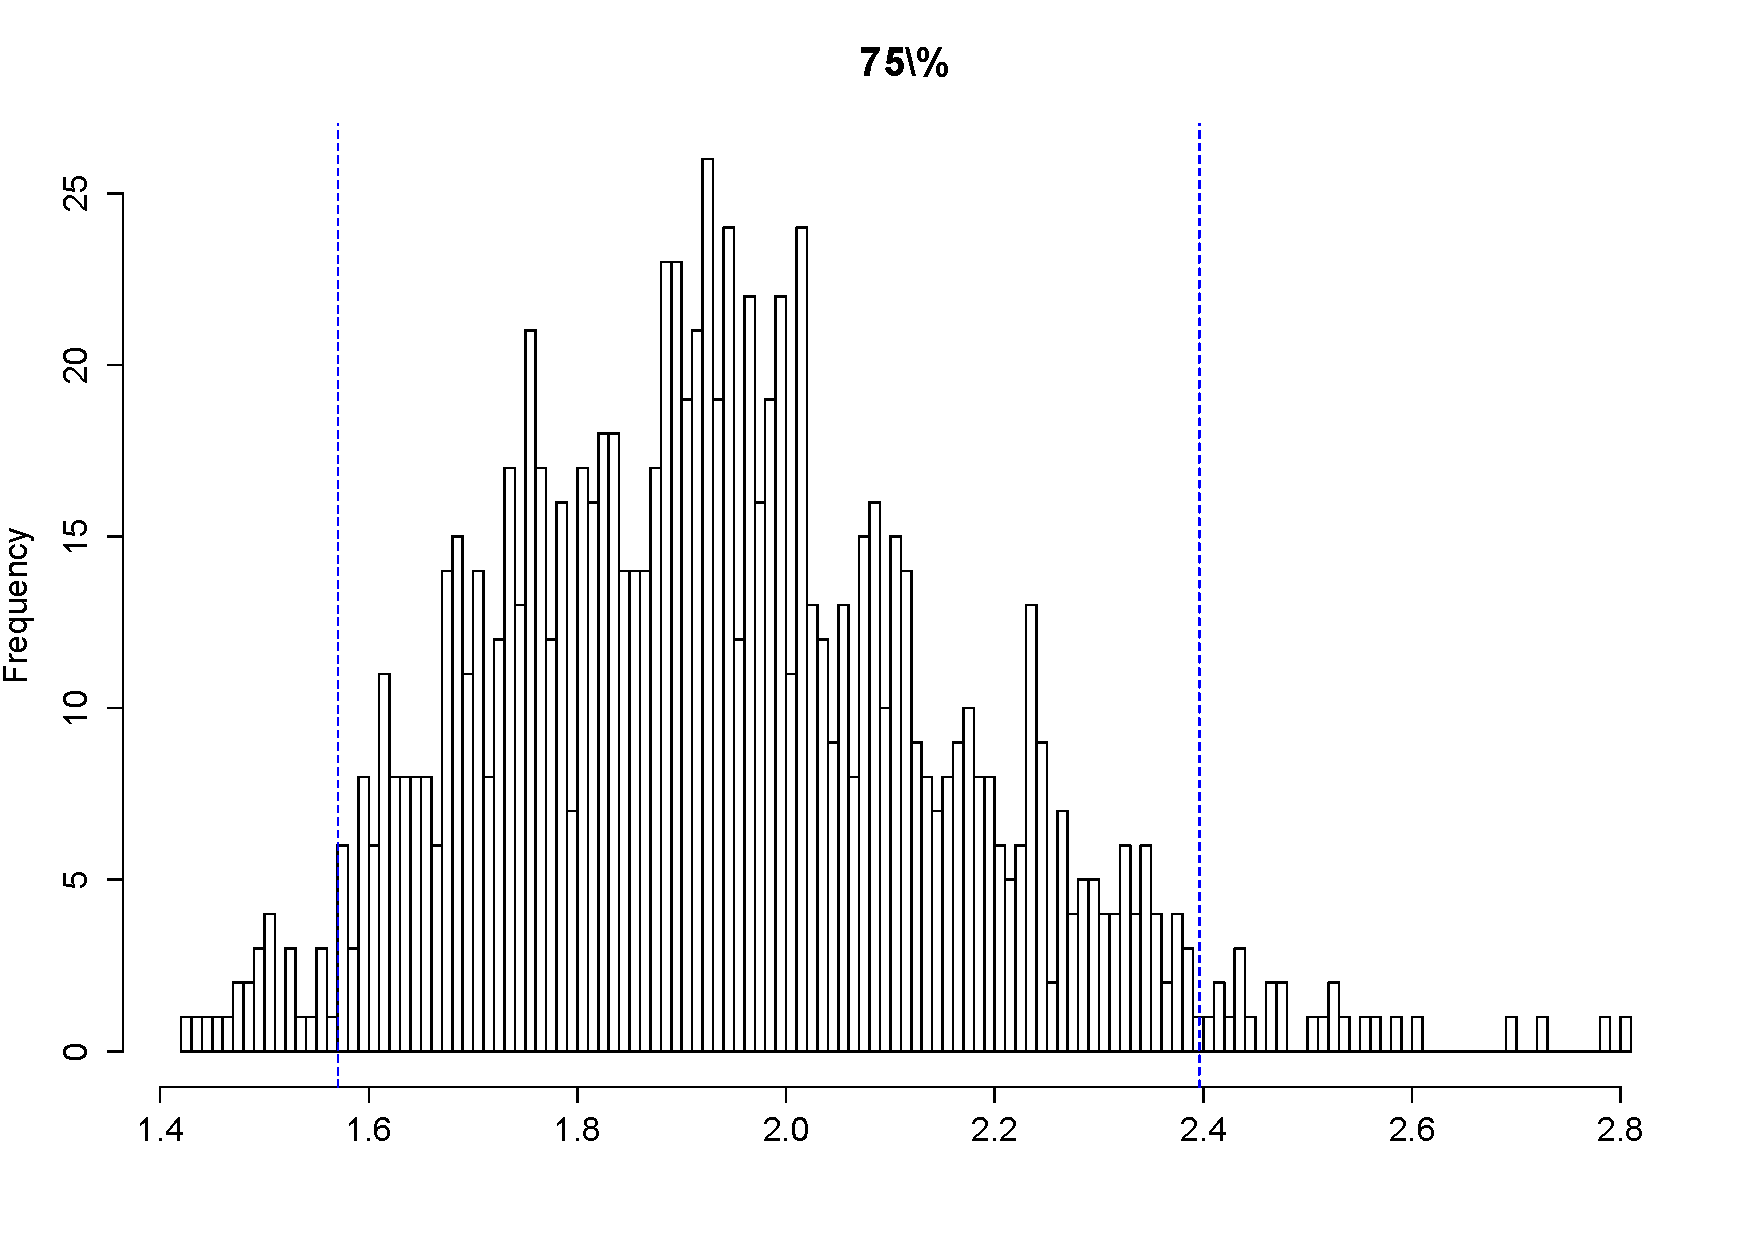
\includegraphics[width = \linewidth]{img/BootstrapAEMV-75-30.pdf}
        \caption{Quantile à 75\%}
        \label{fig:BAEMV75} %BAEMV : bootstrap 2a EMV
    \end{subfigure}%
    \begin{subfigure}[t]{0.3\textwidth}
        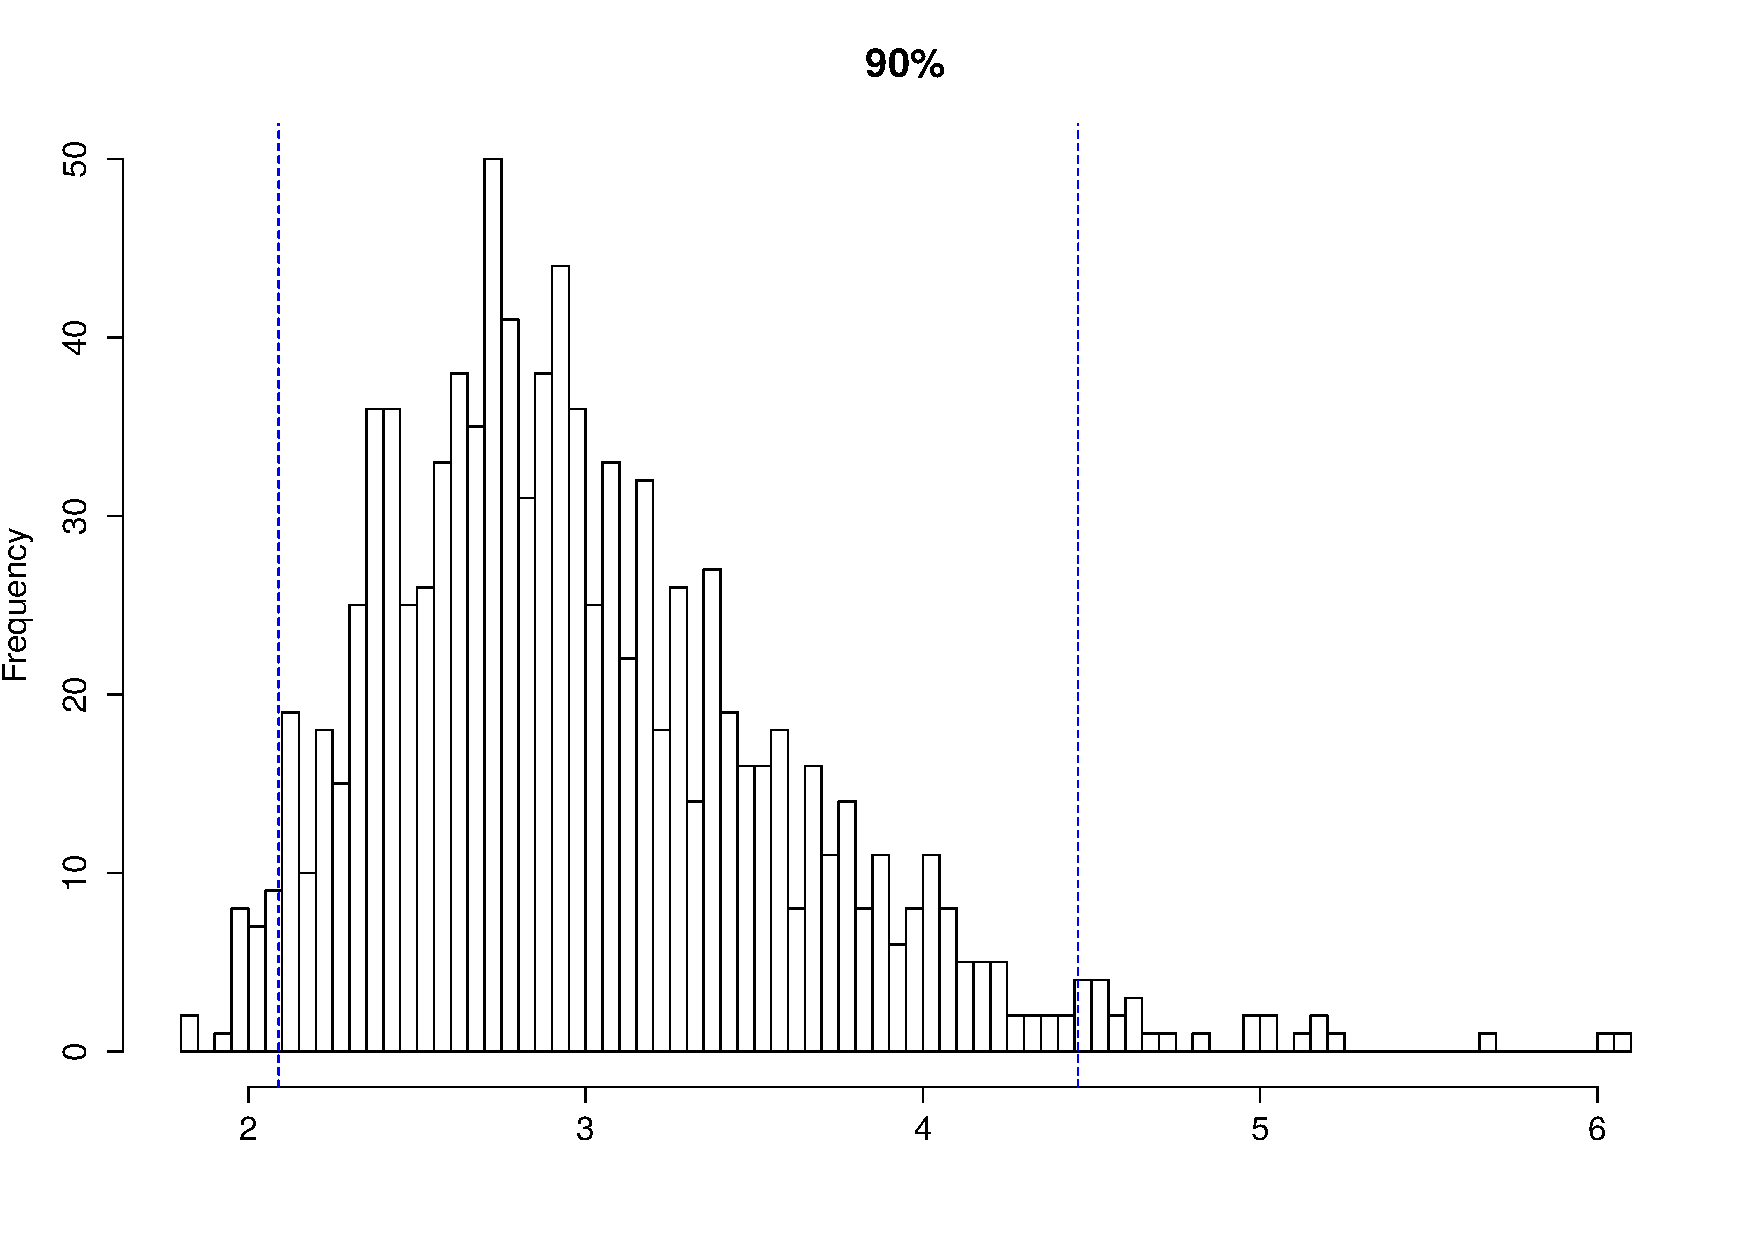
\includegraphics[width = \linewidth]{img/BootstrapAEMV-90-30.pdf}
        \caption{Quantile à 90\%}
        \label{fig:BAEMV90}
    \end{subfigure}%
    \begin{subfigure}[t]{0.3\textwidth}
        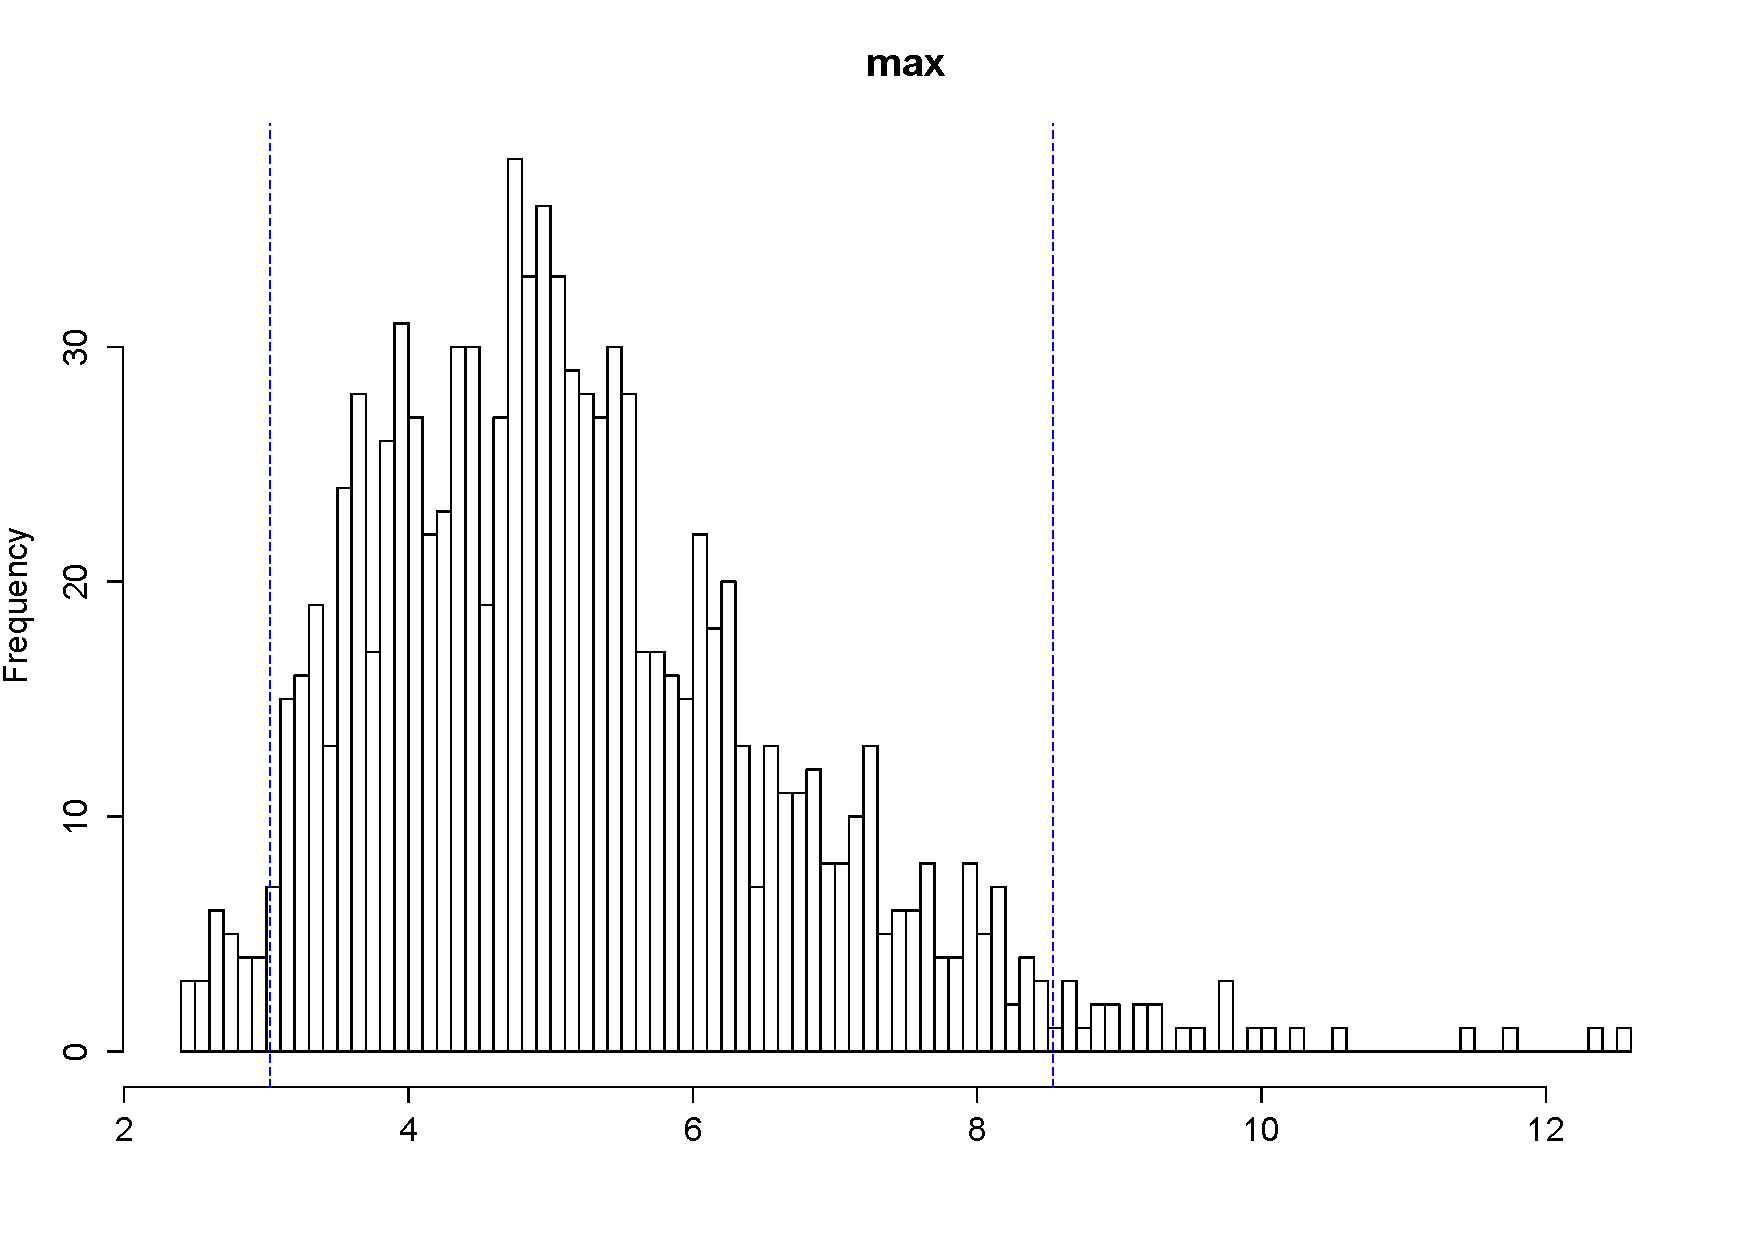
\includegraphics[width = \linewidth]{img/BootstrapAEMV-Max-30.pdf}
        \caption{Quantile à 29/30 : pseudo-maximum empirique}
        \label{fig:BAEMVMax}
    \end{subfigure}%
    \caption{Histogramme de la distribution du quantile estimé par EMV pour n = 30, réalisé par bootstrap naïf}
    \label{fig:BAEMV}
\end{figure}

\begin{figure}[H]
    \centering
    \begin{subfigure}[t]{0.3\textwidth}
        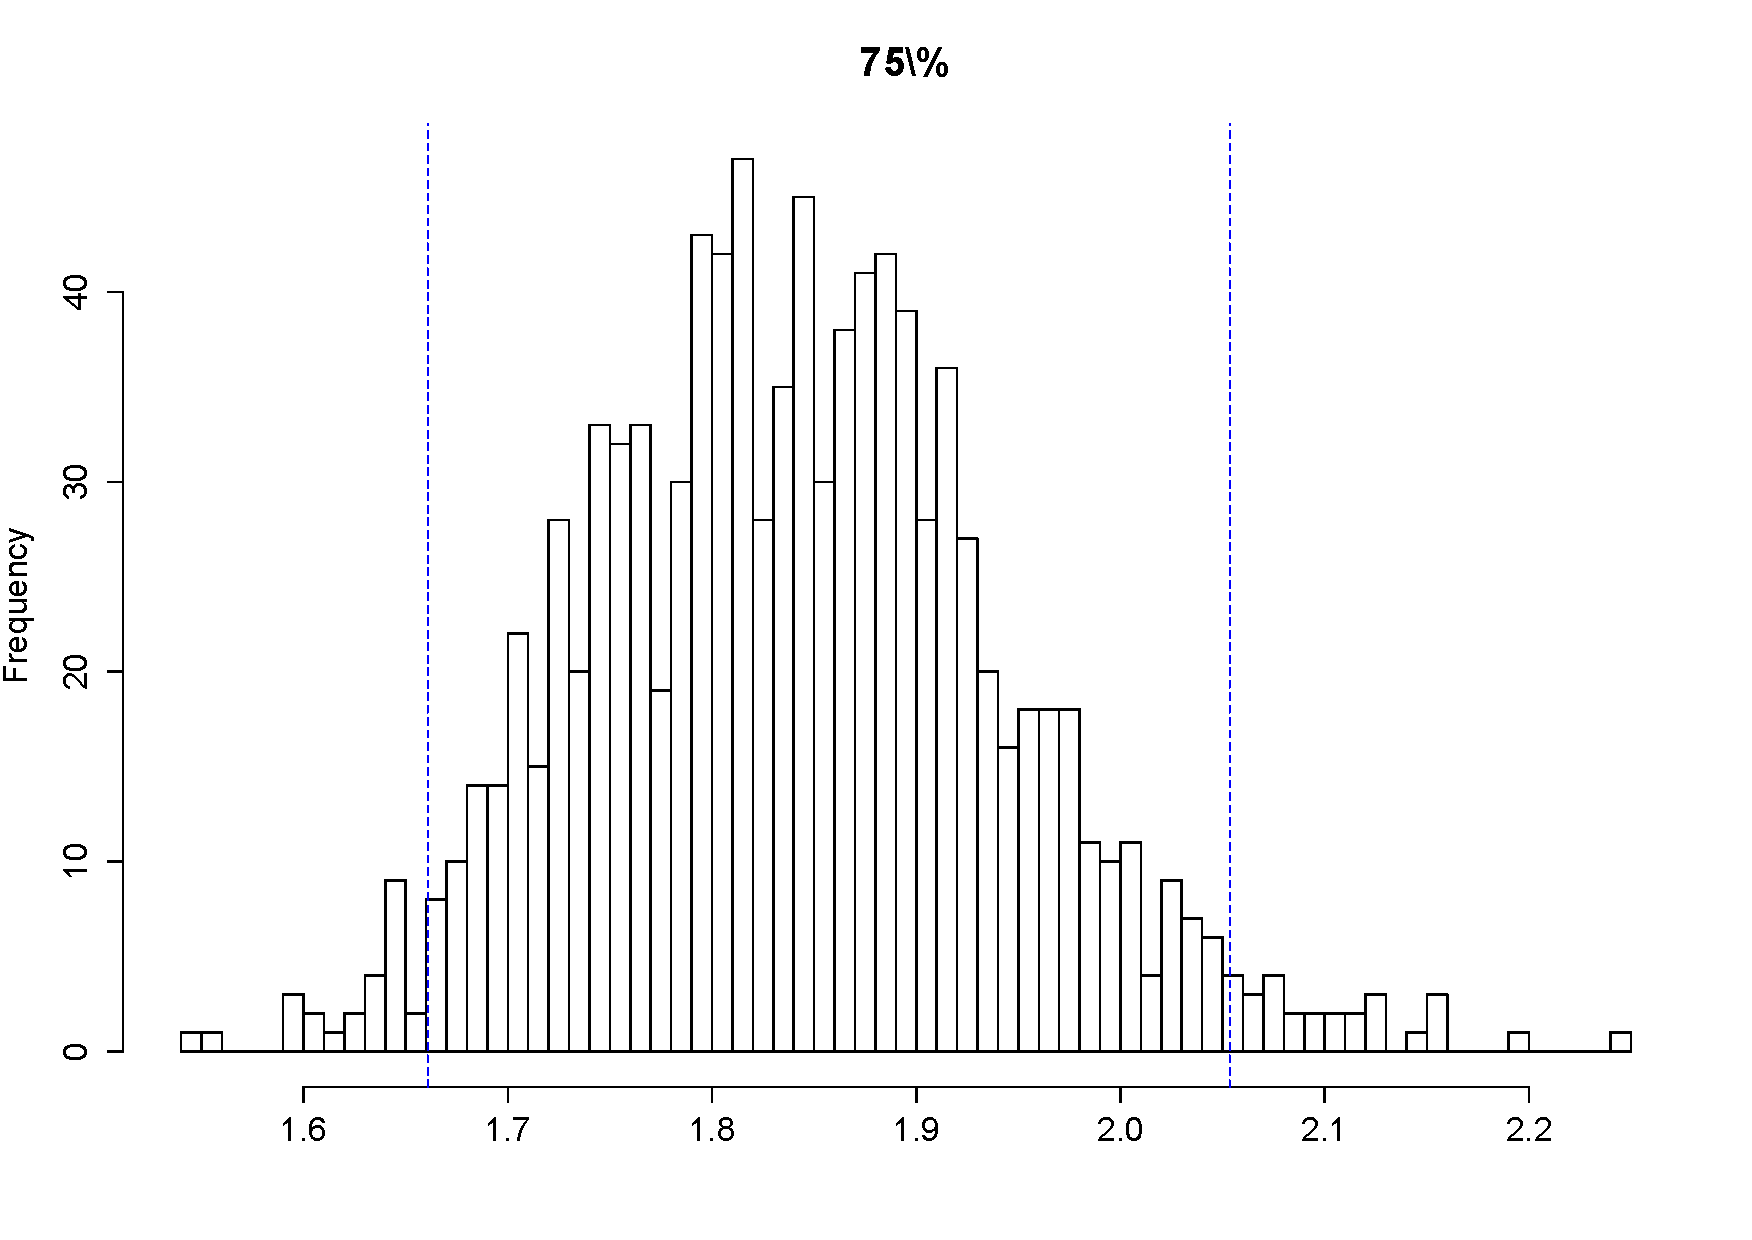
\includegraphics[width = \linewidth]{img/BootstrapAEMV-75-100.pdf}
        \caption{Quantile à 75\%}
        \label{fig:BAEMV75b} %BAEMV : bootstrap 2a EMV
    \end{subfigure}%
    \begin{subfigure}[t]{0.3\textwidth}
        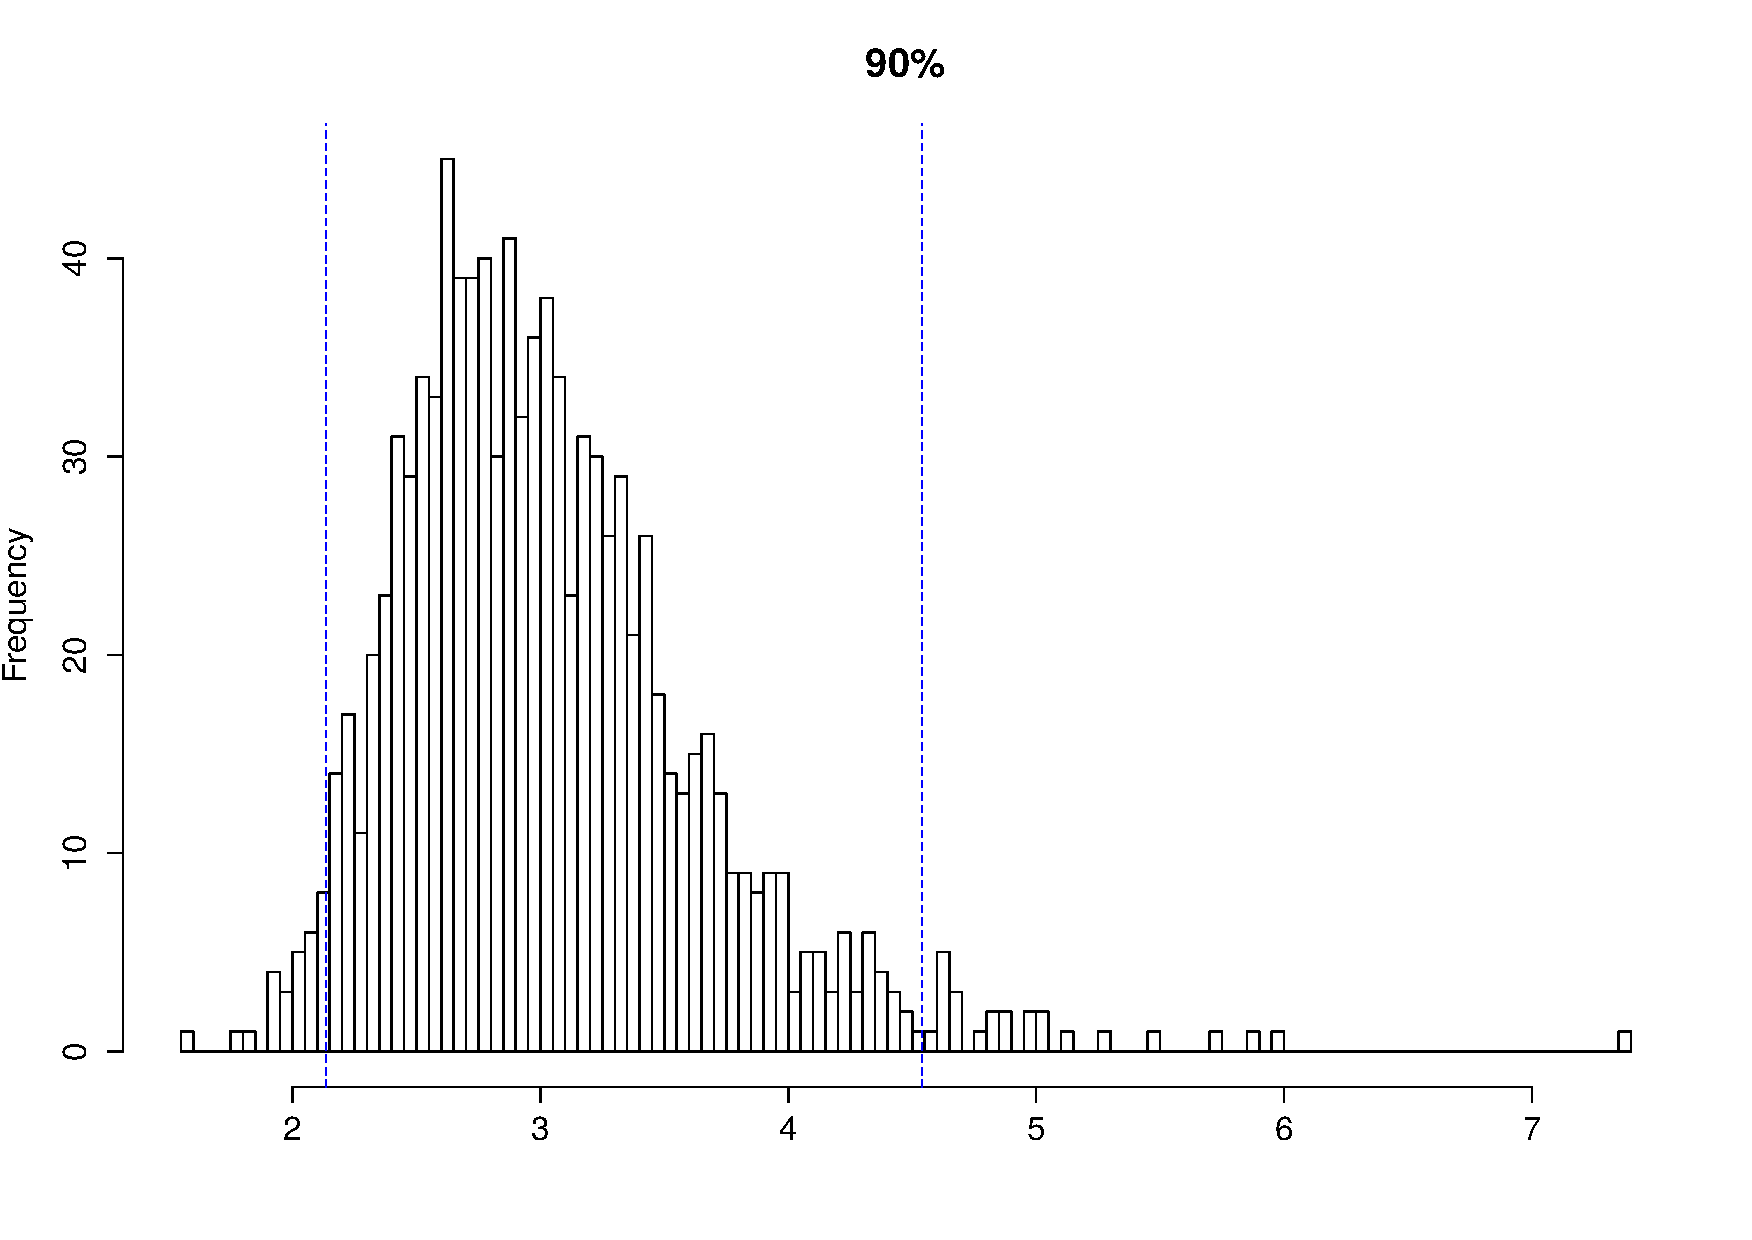
\includegraphics[width = \linewidth]{img/BootstrapAEMV-90-100.pdf}
        \caption{Quantile à 90\%}
        \label{fig:BAEMV90b}
    \end{subfigure}%
    \begin{subfigure}[t]{0.3\textwidth}
        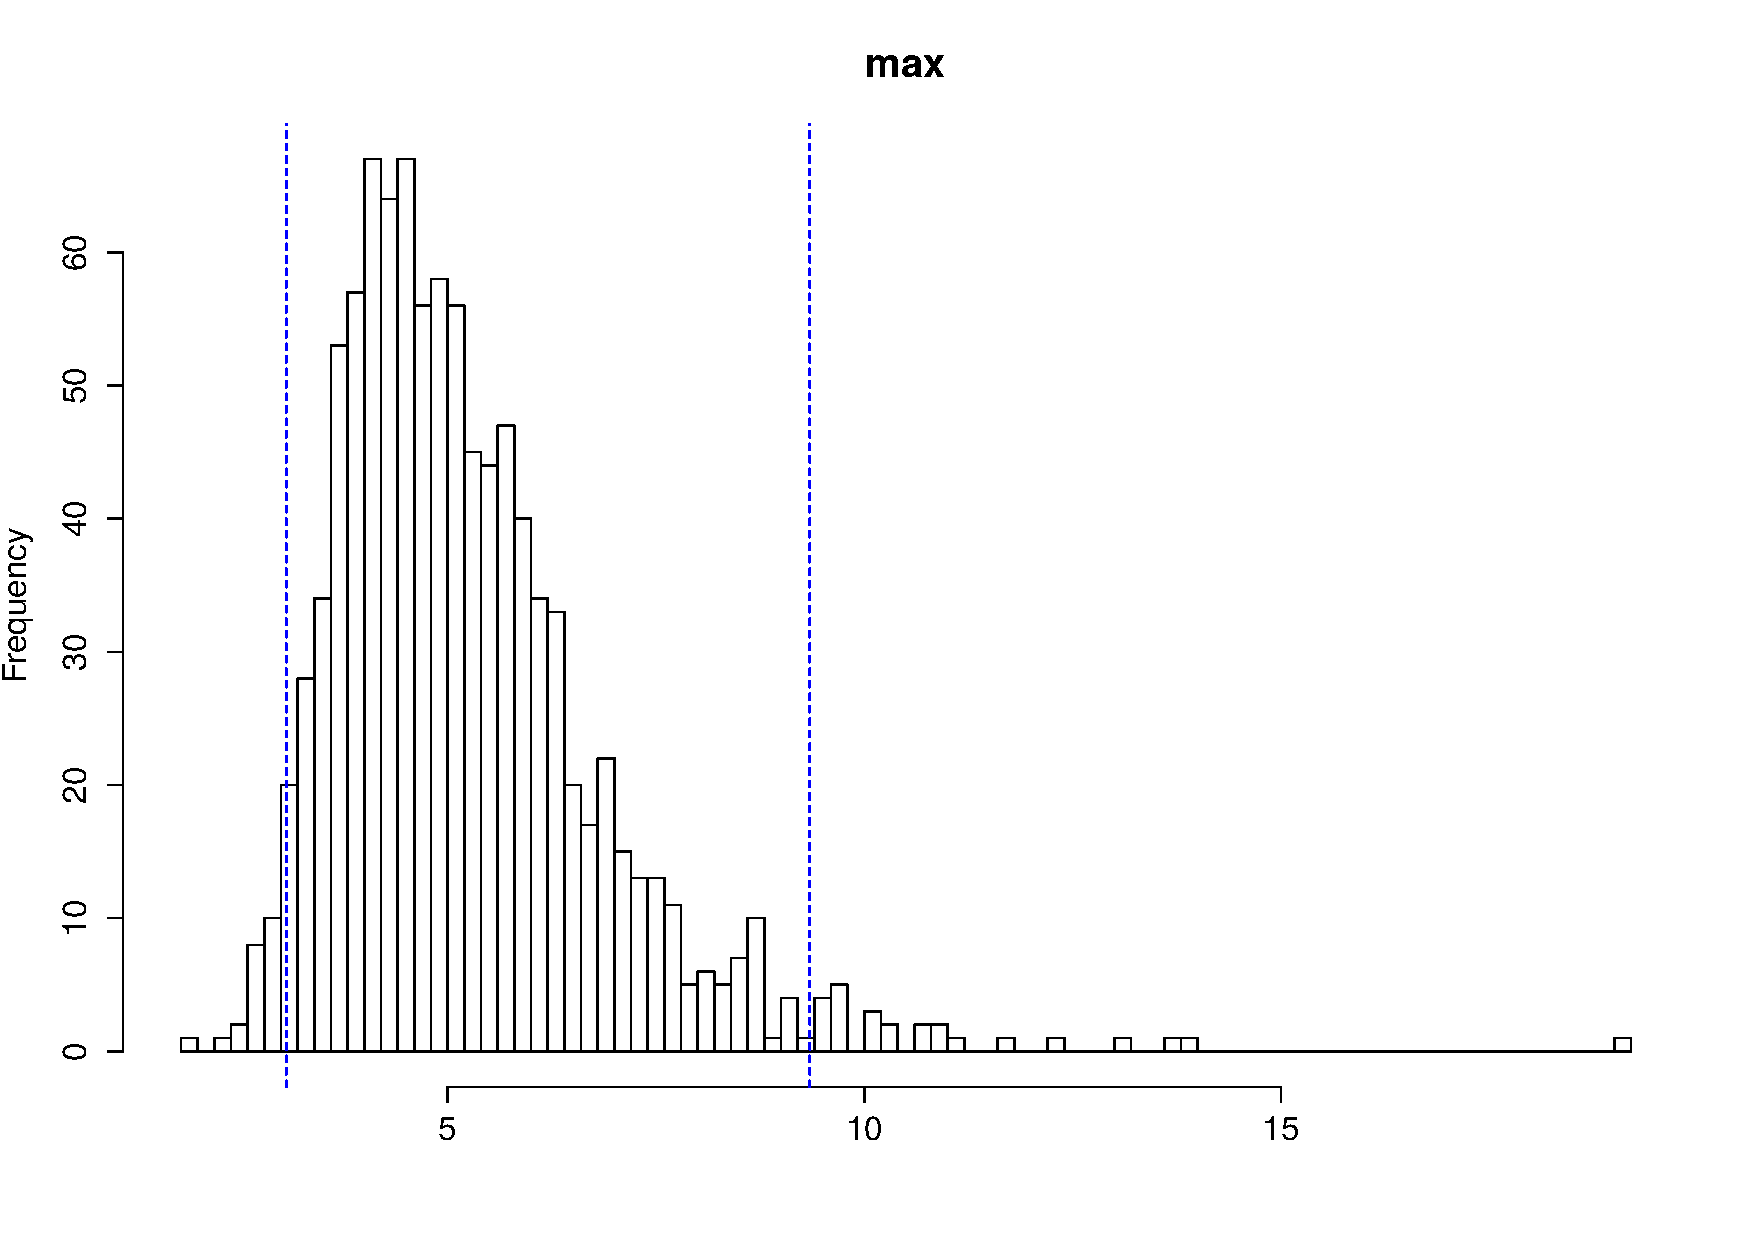
\includegraphics[width = \linewidth]{img/BootstrapAEMV-Max-100.pdf}
        \caption{Quantile à 99/100 : pseudo-maximum empirique}
        \label{fig:BAEMVMaxb}
    \end{subfigure}%
    \caption{Histogramme de la distribution du quantile estimé par EMV pour n = 100, réalisé par bootstrap naïf}
    \label{fig:BAEMVb}
\end{figure}

\subsubsection{Bootstrap paramétrique pour le quantile empirique (1c)}
Dans cette sous-partie on considère à nouveau l'estimateur non-paramétrique du quantile (ou quantile empirique) sur lequel portait la partie 1. On va présenter une nouvelle alternative au bootstrap naïf pour cet estimateur.
L'hypothèse que les données suivent une loi de Pareto de paramètre $\beta$ inconnu permet de réaliser la procédure suivante, dite de \emph{bootstrap paramétrique} :
\begin{enumerate}
\item On calcule l'estimateur $\widehat{\beta}_{MV}(X)$
\item On simule $B$ échantillons de taille $n$ et de même loi : 
\[\forall b = 1,..,B, \ X^{*b} = (X^*_{1^b}, ..., X^*_{n^b}) \sim Pareto(\widehat{\beta}_{MV}(X)) \]
\item On calcule le quantile empirique $\widehat{Q(q)}_b$ de chacun de ces échantillons. On obtient ainsi un échantillon de taille $b$ d'estimateurs du quantile empirique. 
\end{enumerate}
Le bootstrap paramétrique est une façon de lisser la loi $F_n$ selon laquelle les échantillons de bootstrap sont tirés, puisqu'il s'agit ici d'une loi de Pareto. Contrairement à la fonction de répartition empirique utilisée dans un bootstrap naïf, cette loi est absolument continue par rapport à la mesure de Lebesgue donc la fonction d'influence de l'opérateur quantile \eqref{influenceQ} y est bien définie, ce qui rend possible la validité du bootstrap au second ordre. \\ 

En revanche cette méthode est peu robuste puisque pour qu'elle impose que $X$ suive véritablement une loi de Pareto. Dans le cas contraire $F_n$ ne tend pas vers $F$ et le bootstrap ne converge pas. \\ 
Paralèllement au bootstrap, la variance asymptotique du quantile empirique, dont on avait une expression théorique \eqref{var1} lors de l'estimation non-paramétrique, peut désormais être estimée en remplaçant $\beta_0$ par $\widehat{\beta}_{MV}(X))$ dans cette formule, on estime ainsi de nouveaux intervalles de confiance asymptotique du quantile empirique.
\begin{table}[H]
\centering
\begin{tabular}{c|c|ccccc}
&Théorique&IC Oracle &IC Matthieu avec Beta hat EMV&IC Matthieu avec Beta hat Hill&IC EMV&IC Hill\\
\hline
75\%&2&\begin{tabular}{c}$1.76$\\{\small $[ 1.61 , 1.91 ]$ } \end{tabular}&\begin{tabular}{c}$1.94$\\{\small $[ 1.88 , 2 ]$ } \end{tabular}&\begin{tabular}{c}$1.94$\\{\small $[ 1.87 , 2 ]$ } \end{tabular}&\begin{tabular}{c}$1.96$\\{\small $[ 1.5 , 2.68 ]$ } \end{tabular}&\begin{tabular}{c}$1.98$\\{\small $[ 1.51 , 2.74 ]$ } \end{tabular}\\
90\%&3.16&\begin{tabular}{c}$2.66$\\{\small $[ 2.2 , 3.12 ]$ } \end{tabular}&\begin{tabular}{c}$2.42$\\{\small $[ 2.31 , 2.54 ]$ } \end{tabular}&\begin{tabular}{c}$2.42$\\{\small $[ 2.3 , 2.54 ]$ } \end{tabular}&\begin{tabular}{c}$2.87$\\{\small $[ 1.89 , 4.66 ]$ } \end{tabular}&\begin{tabular}{c}$2.89$\\{\small $[ 1.88 , 4.81 ]$ } \end{tabular}\\
max&5.48&\begin{tabular}{c}$6.57$\\{\small $[ 1.52 , 11.62 ]$ } \end{tabular}&\begin{tabular}{c}$4.18$\\{\small $[ 3.96 , 4.39 ]$ } \end{tabular}&\begin{tabular}{c}$4.18$\\{\small $[ 3.96 , 4.39 ]$ } \end{tabular}&\begin{tabular}{c}$4.48$\\{\small $[ 2.31 , 9.56 ]$ } \end{tabular}&\begin{tabular}{c}$4.52$\\{\small $[ 2.31 , 9.95 ]$ } \end{tabular}
\end{tabular}
\caption{n = 30}
\label{tab:resPram30}
\end{table} 

\begin{table}[H]
\centering
\begin{tabular}{c|c|ccccc}
&Théorique&IC Oracle &IC Matthieu avec Beta hat EMV&IC Matthieu avec Beta hat Hill&IC EMV&IC Hill\\
\hline
75\%&2&\begin{tabular}{c}$1.76$\\{\small $[ 1.61 , 1.91 ]$ } \end{tabular}&\begin{tabular}{c}$1.76$\\{\small $[ 1.73 , 1.79 ]$ } \end{tabular}&\begin{tabular}{c}$1.76$\\{\small $[ 1.73 , 1.79 ]$ } \end{tabular}&\begin{tabular}{c}$1.83$\\{\small $[ 1.59 , 2.14 ]$ } \end{tabular}&\begin{tabular}{c}$1.76$\\{\small $[ 1.55 , 2.03 ]$ } \end{tabular}\\
90\%&3.16&\begin{tabular}{c}$2.66$\\{\small $[ 2.2 , 3.12 ]$ } \end{tabular}&\begin{tabular}{c}$2.66$\\{\small $[ 2.6 , 2.72 ]$ } \end{tabular}&\begin{tabular}{c}$2.66$\\{\small $[ 2.61 , 2.71 ]$ } \end{tabular}&\begin{tabular}{c}$2.72$\\{\small $[ 2.14 , 3.54 ]$ } \end{tabular}&\begin{tabular}{c}$2.56$\\{\small $[ 2.04 , 3.28 ]$ } \end{tabular}\\
max&10&\begin{tabular}{c}$6.57$\\{\small $[ 1.52 , 11.62 ]$ } \end{tabular}&\begin{tabular}{c}$6.57$\\{\small $[ 6.4 , 6.74 ]$ } \end{tabular}&\begin{tabular}{c}$6.57$\\{\small $[ 6.43 , 6.71 ]$ } \end{tabular}&\begin{tabular}{c}$6.72$\\{\small $[ 3.59 , 14.25 ]$ } \end{tabular}&\begin{tabular}{c}$5.96$\\{\small $[ 3.32 , 11.97 ]$ } \end{tabular}
\end{tabular}
\caption{n = 100}
\label{tab:resParam100}
\end{table} 

%%Ne serait-il pas plus pertinent de comparer Hill et EMV, plutot que de comparer EMV a la théorie et Hill a la théorie ?
%%La on se tape 4 tableaux dans la partie de Matthieu, pour moi c'est illisible !

\begin{figure}[H]
    \centering
    \begin{subfigure}[t]{0.3\textwidth}
        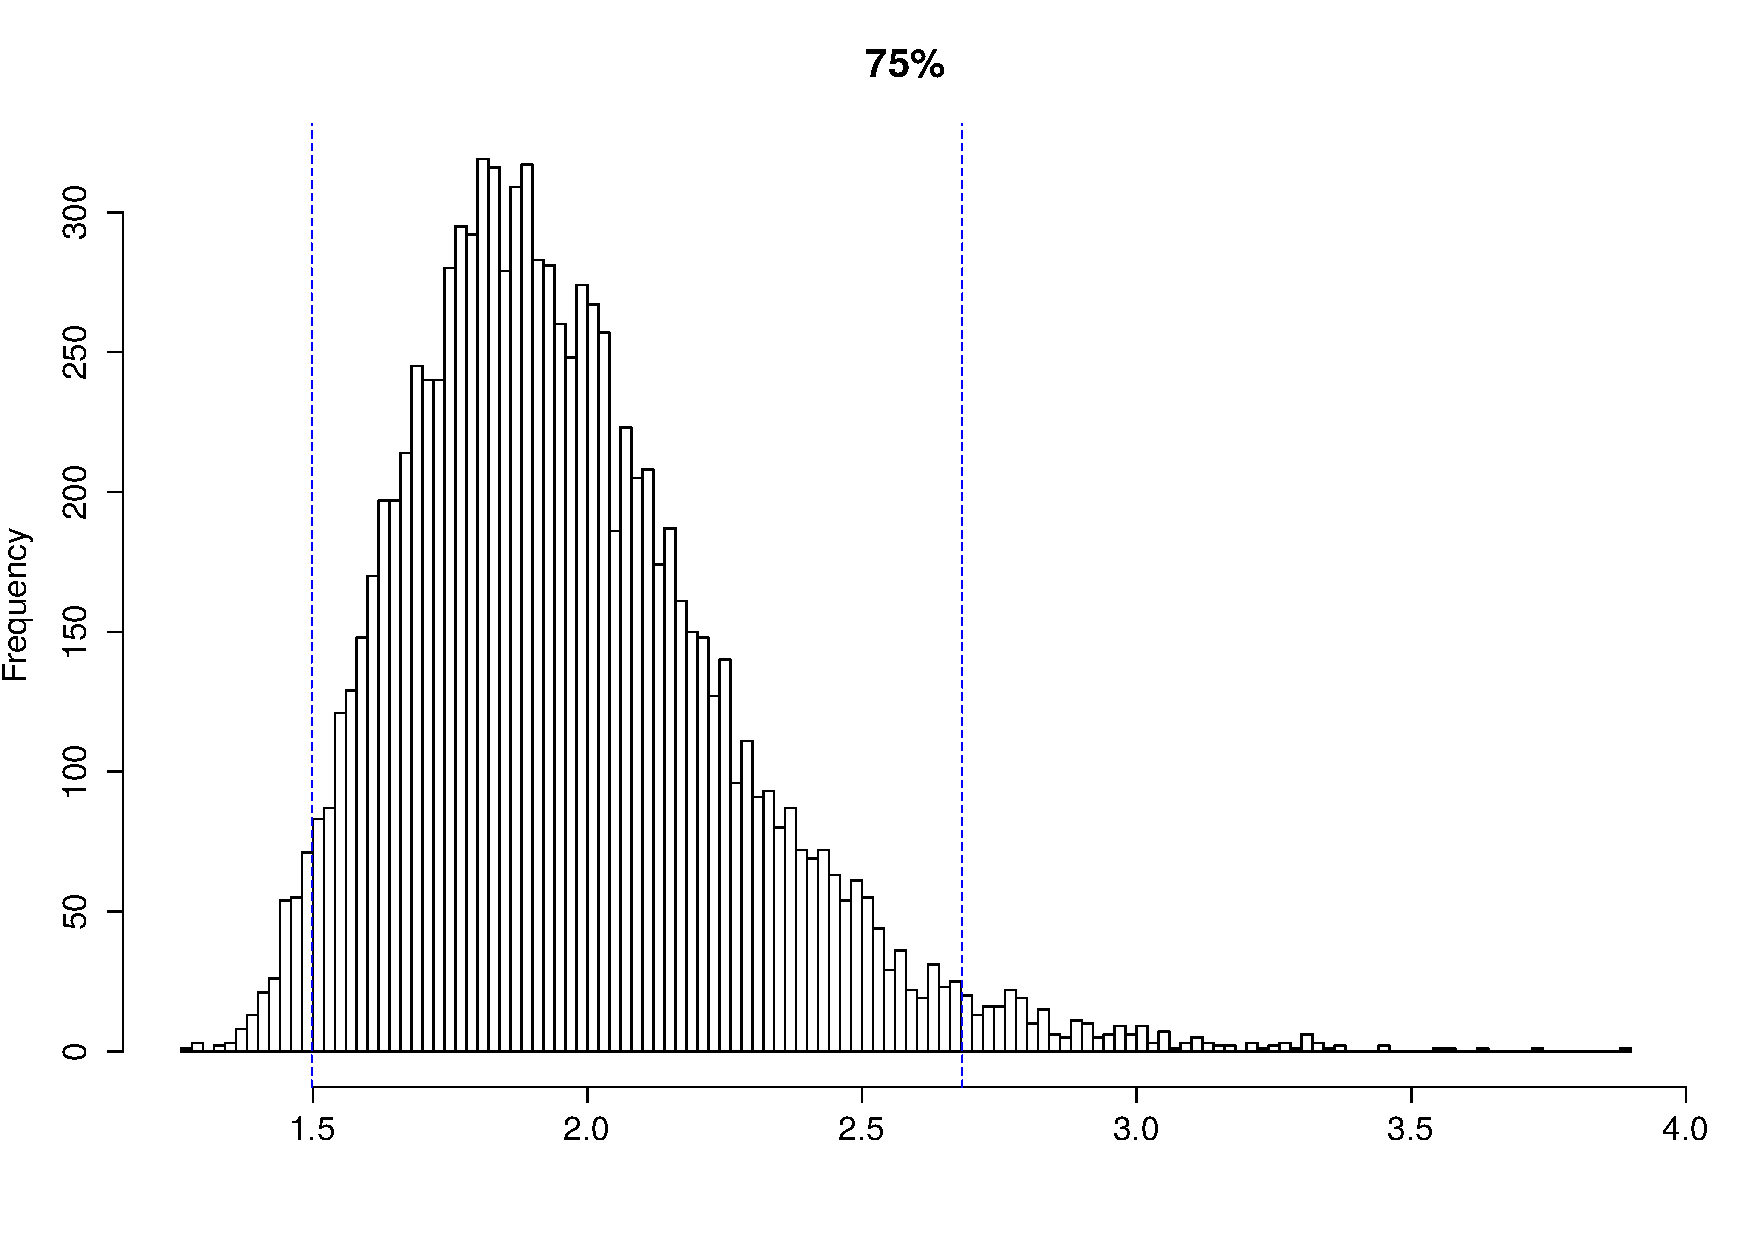
\includegraphics[width = \linewidth]{img/BootstrapParamEMV-75-30.pdf}
        \caption{Quantile à 75\%}
        \label{fig:BPEMV75} %BPEMV : bootstrap parametrique EMV
    \end{subfigure}%
    \begin{subfigure}[t]{0.3\textwidth}
        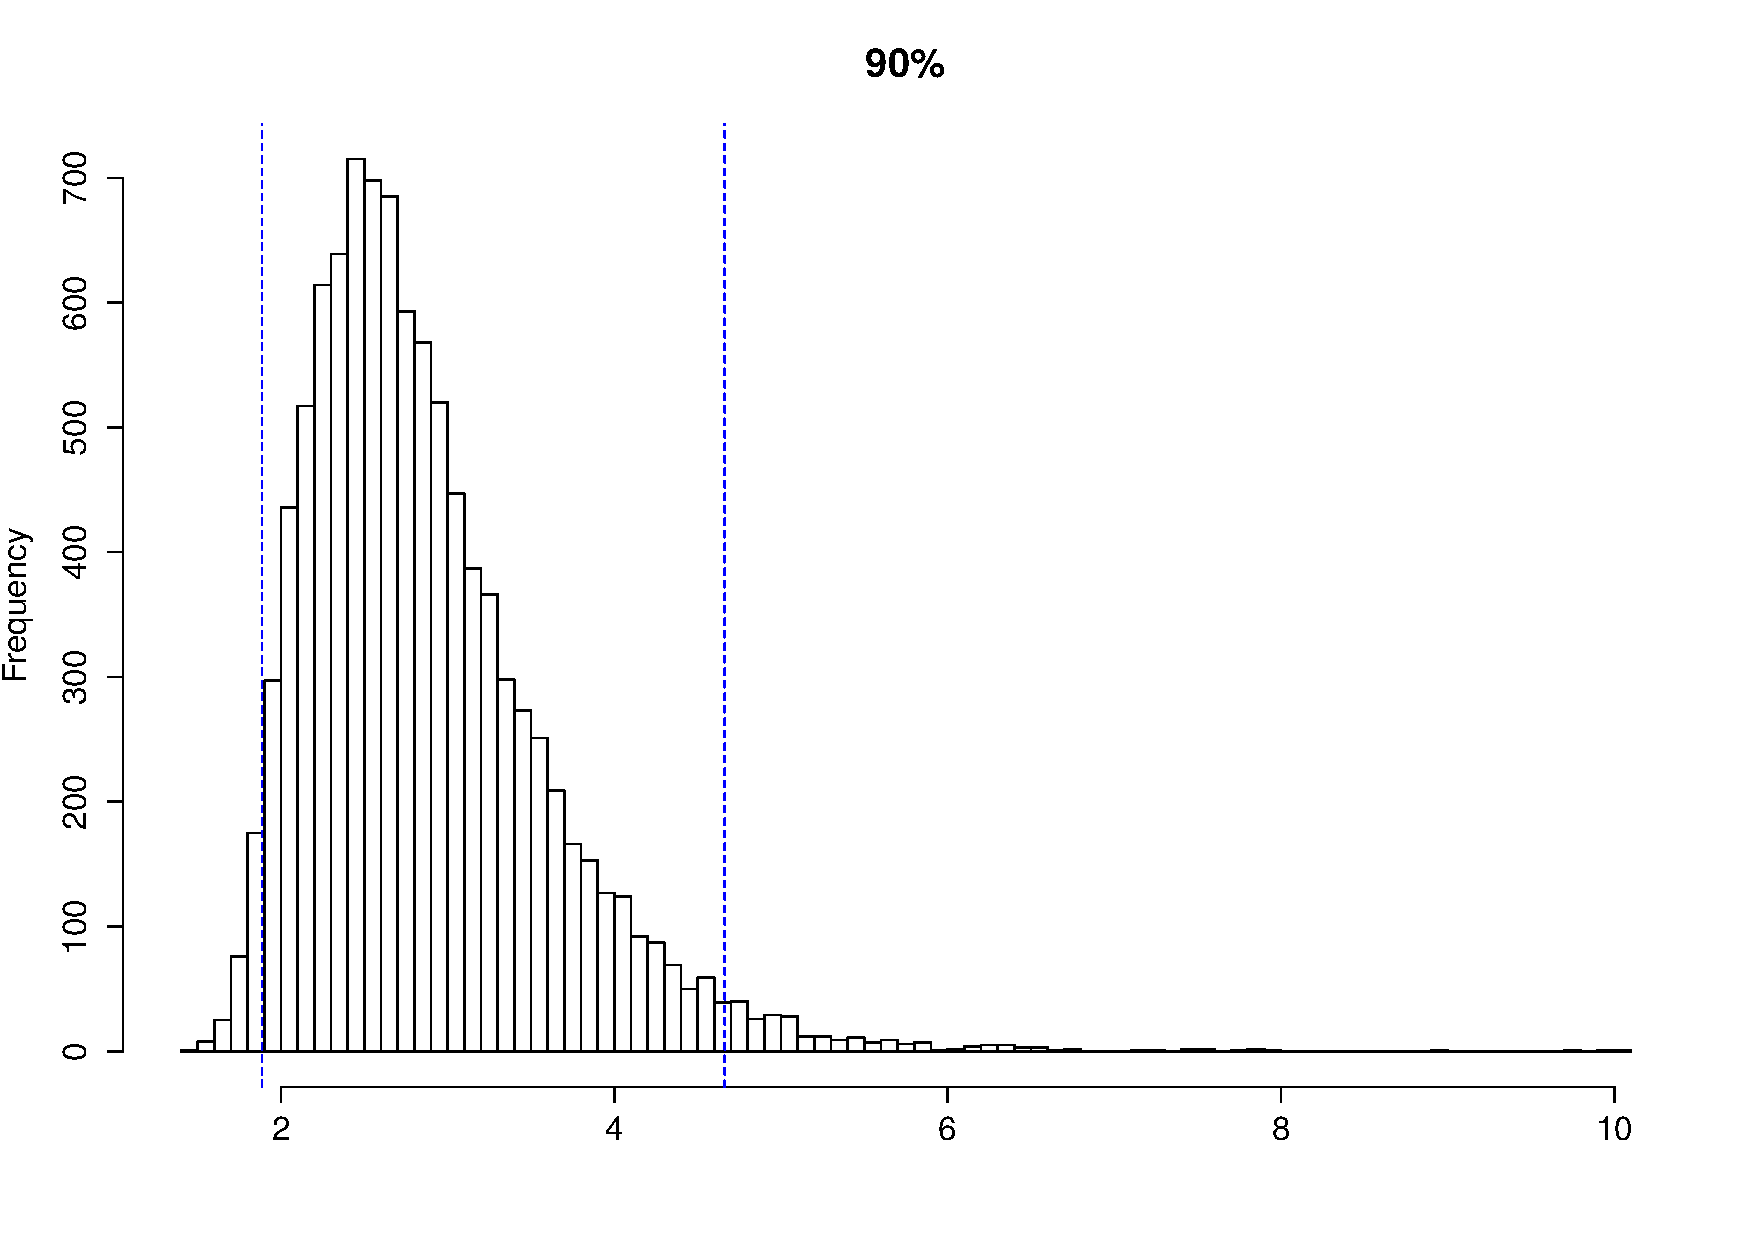
\includegraphics[width = \linewidth]{img/BootstrapParamEMV-90-30.pdf}
        \caption{Quantile à 90\%}
        \label{fig:BPEMV90}
    \end{subfigure}%
    \begin{subfigure}[t]{0.3\textwidth}
        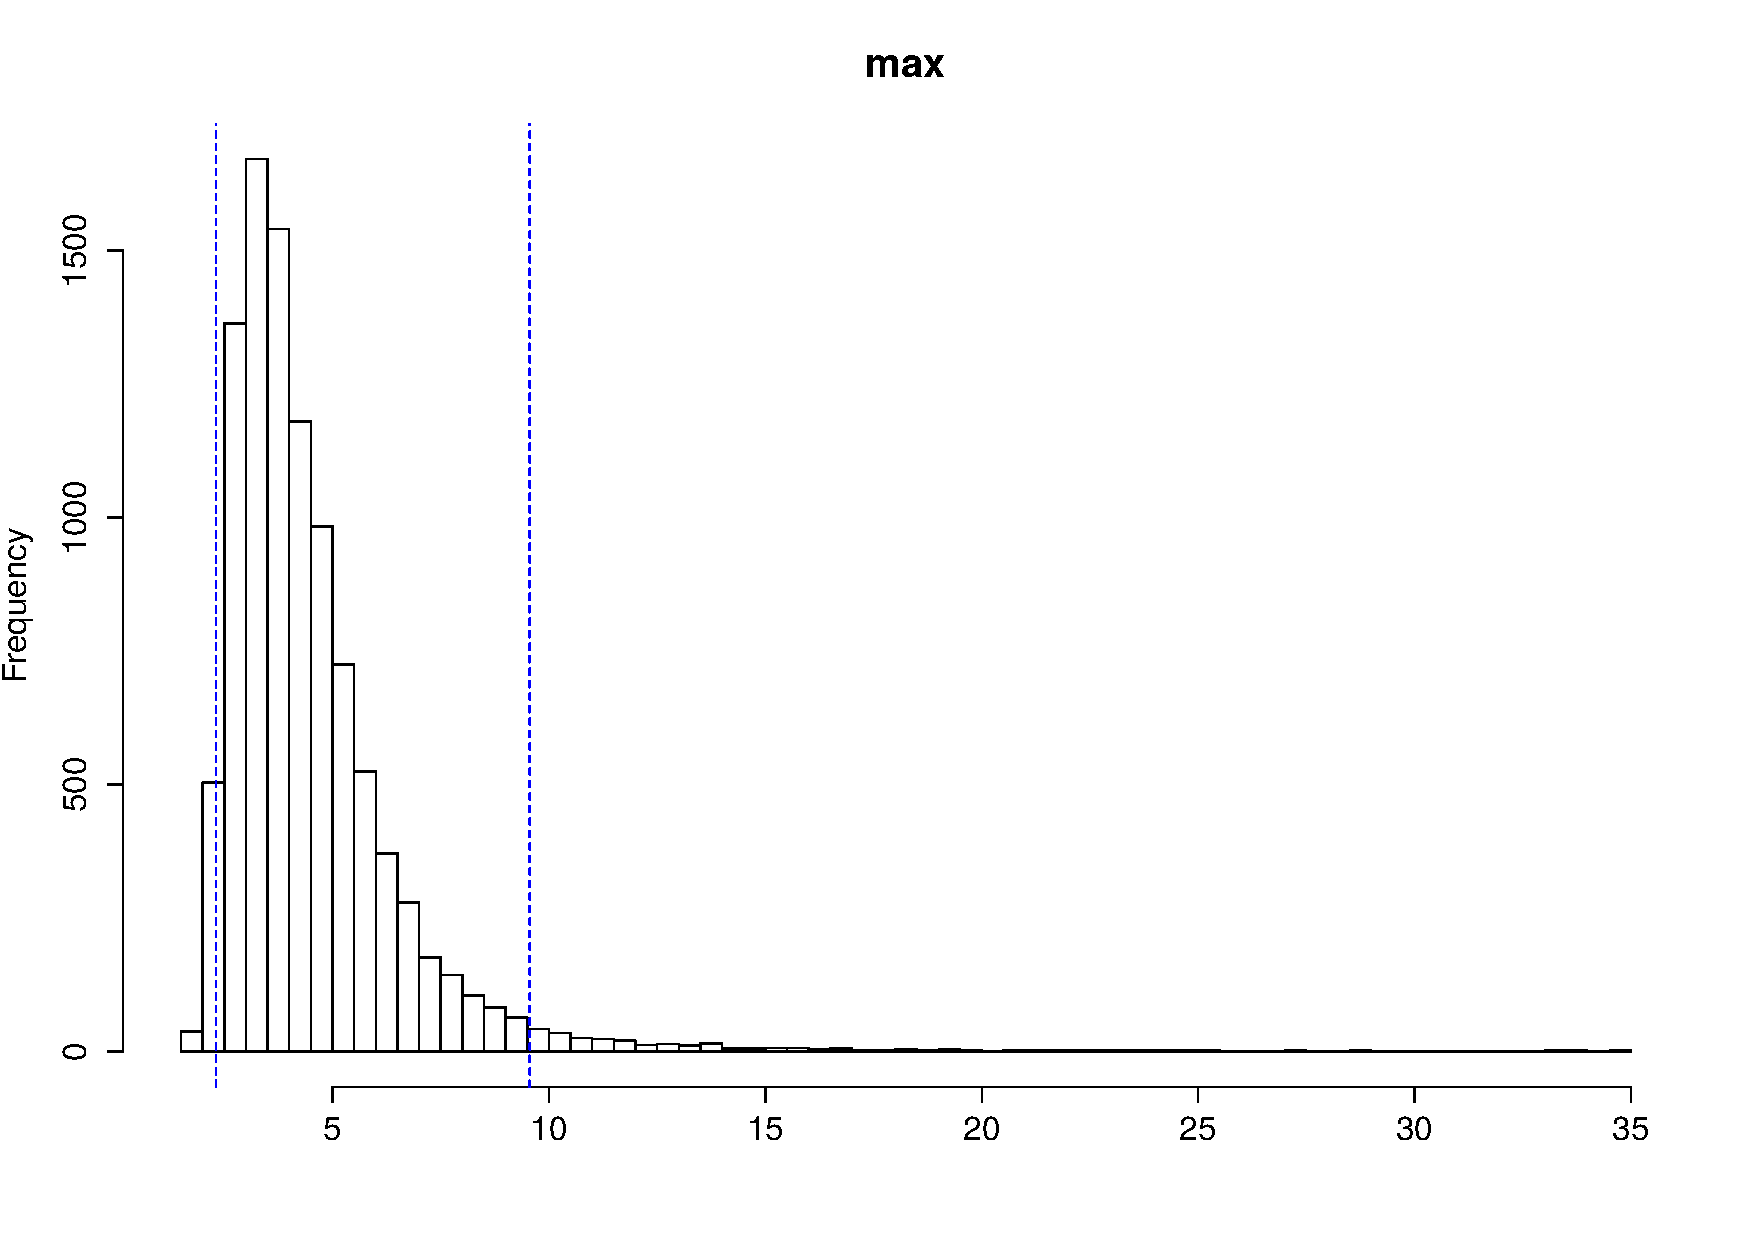
\includegraphics[width = \linewidth]{img/BootstrapParamEMV-Max-30.pdf}
        \caption{Quantile à 29/30 : maximum empirique}
        \label{fig:BPEMVMax}
    \end{subfigure}%
    \caption{Histogramme de la distribution du quantile empirique pour n = 30, obtenu par bootstrap paramétrique}
    \label{fig:BPEMV}
\end{figure}

\begin{figure}[H]
    \centering
    \begin{subfigure}[t]{0.3\textwidth}
        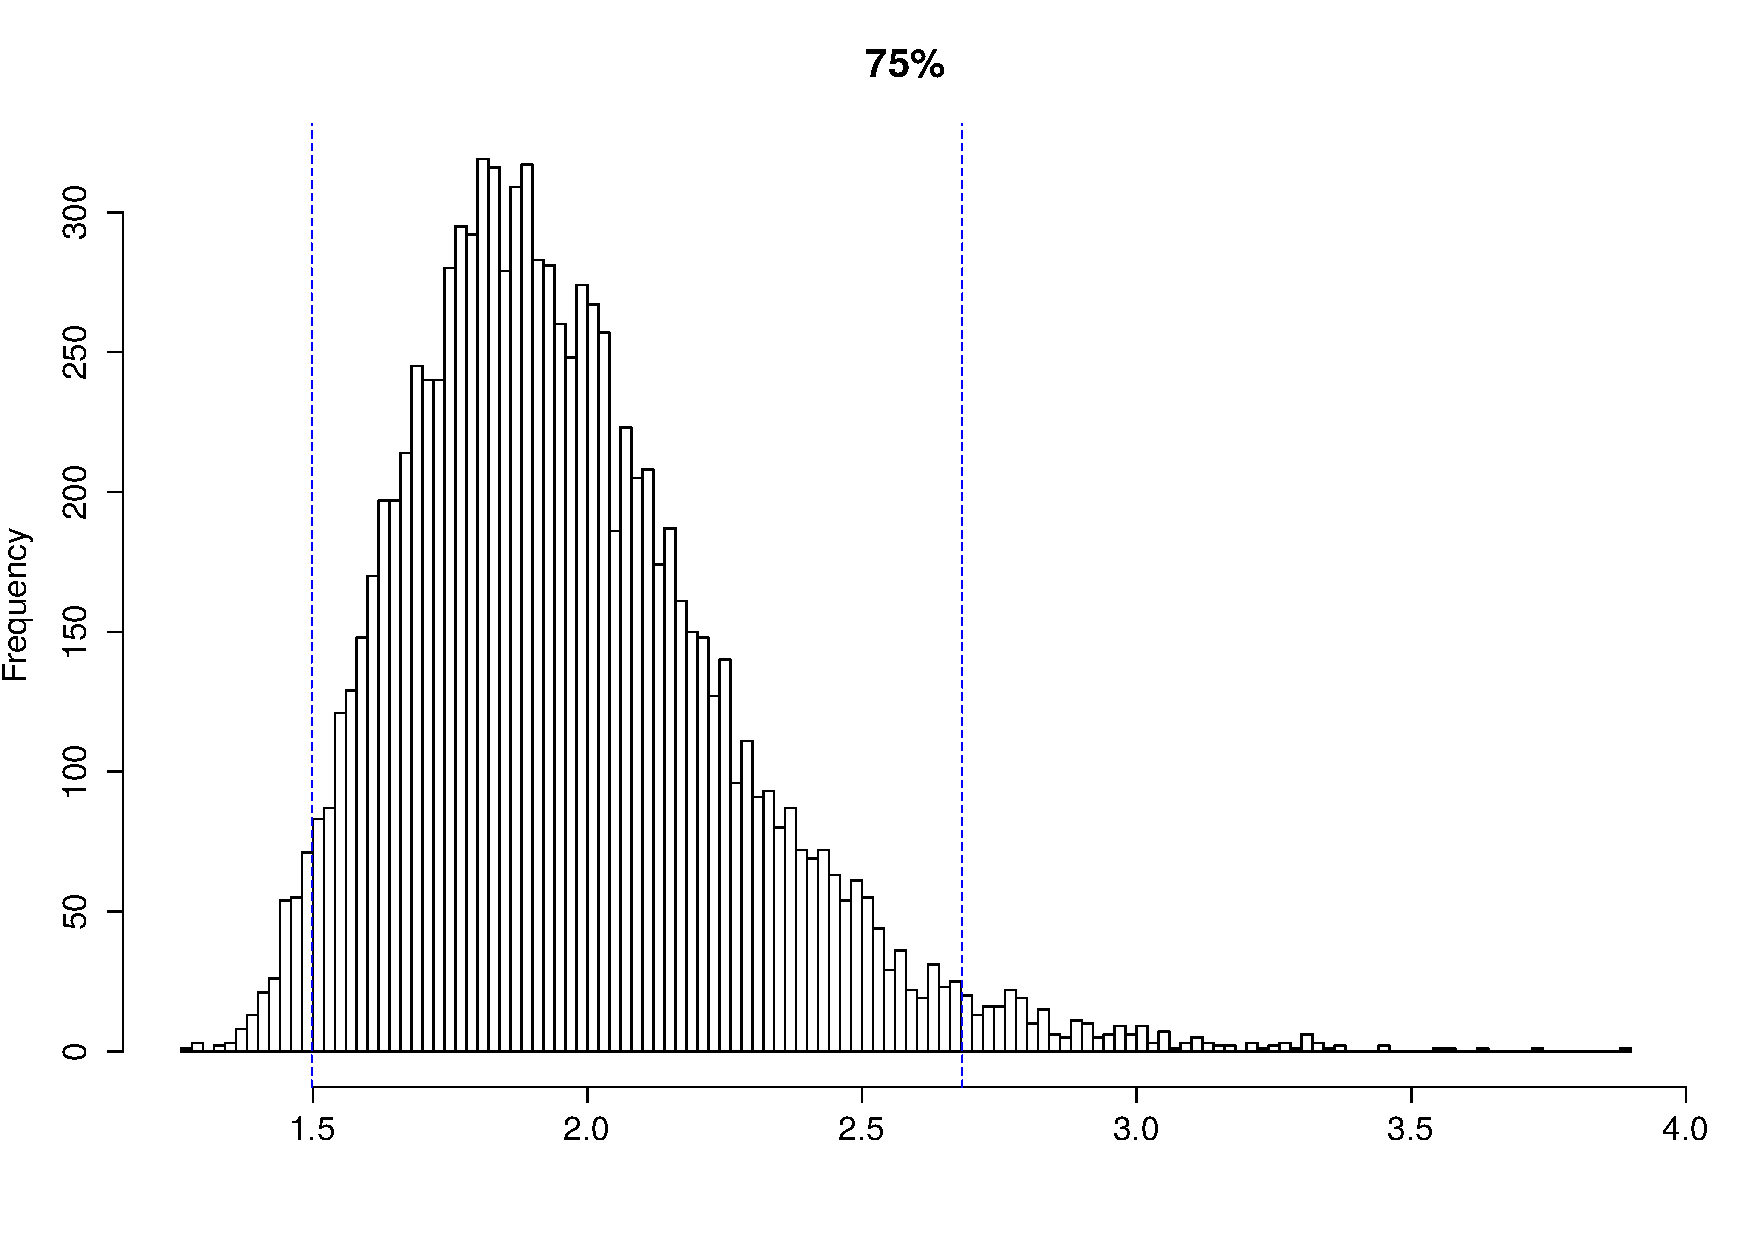
\includegraphics[width = \linewidth]{img/BootstrapParamEMV-75-100.pdf}
        \caption{Quantile à 75\%}
        \label{fig:BPEMV75b} %BPEMV : bootstrap parametrique EMV
    \end{subfigure}%
    \begin{subfigure}[t]{0.3\textwidth}
        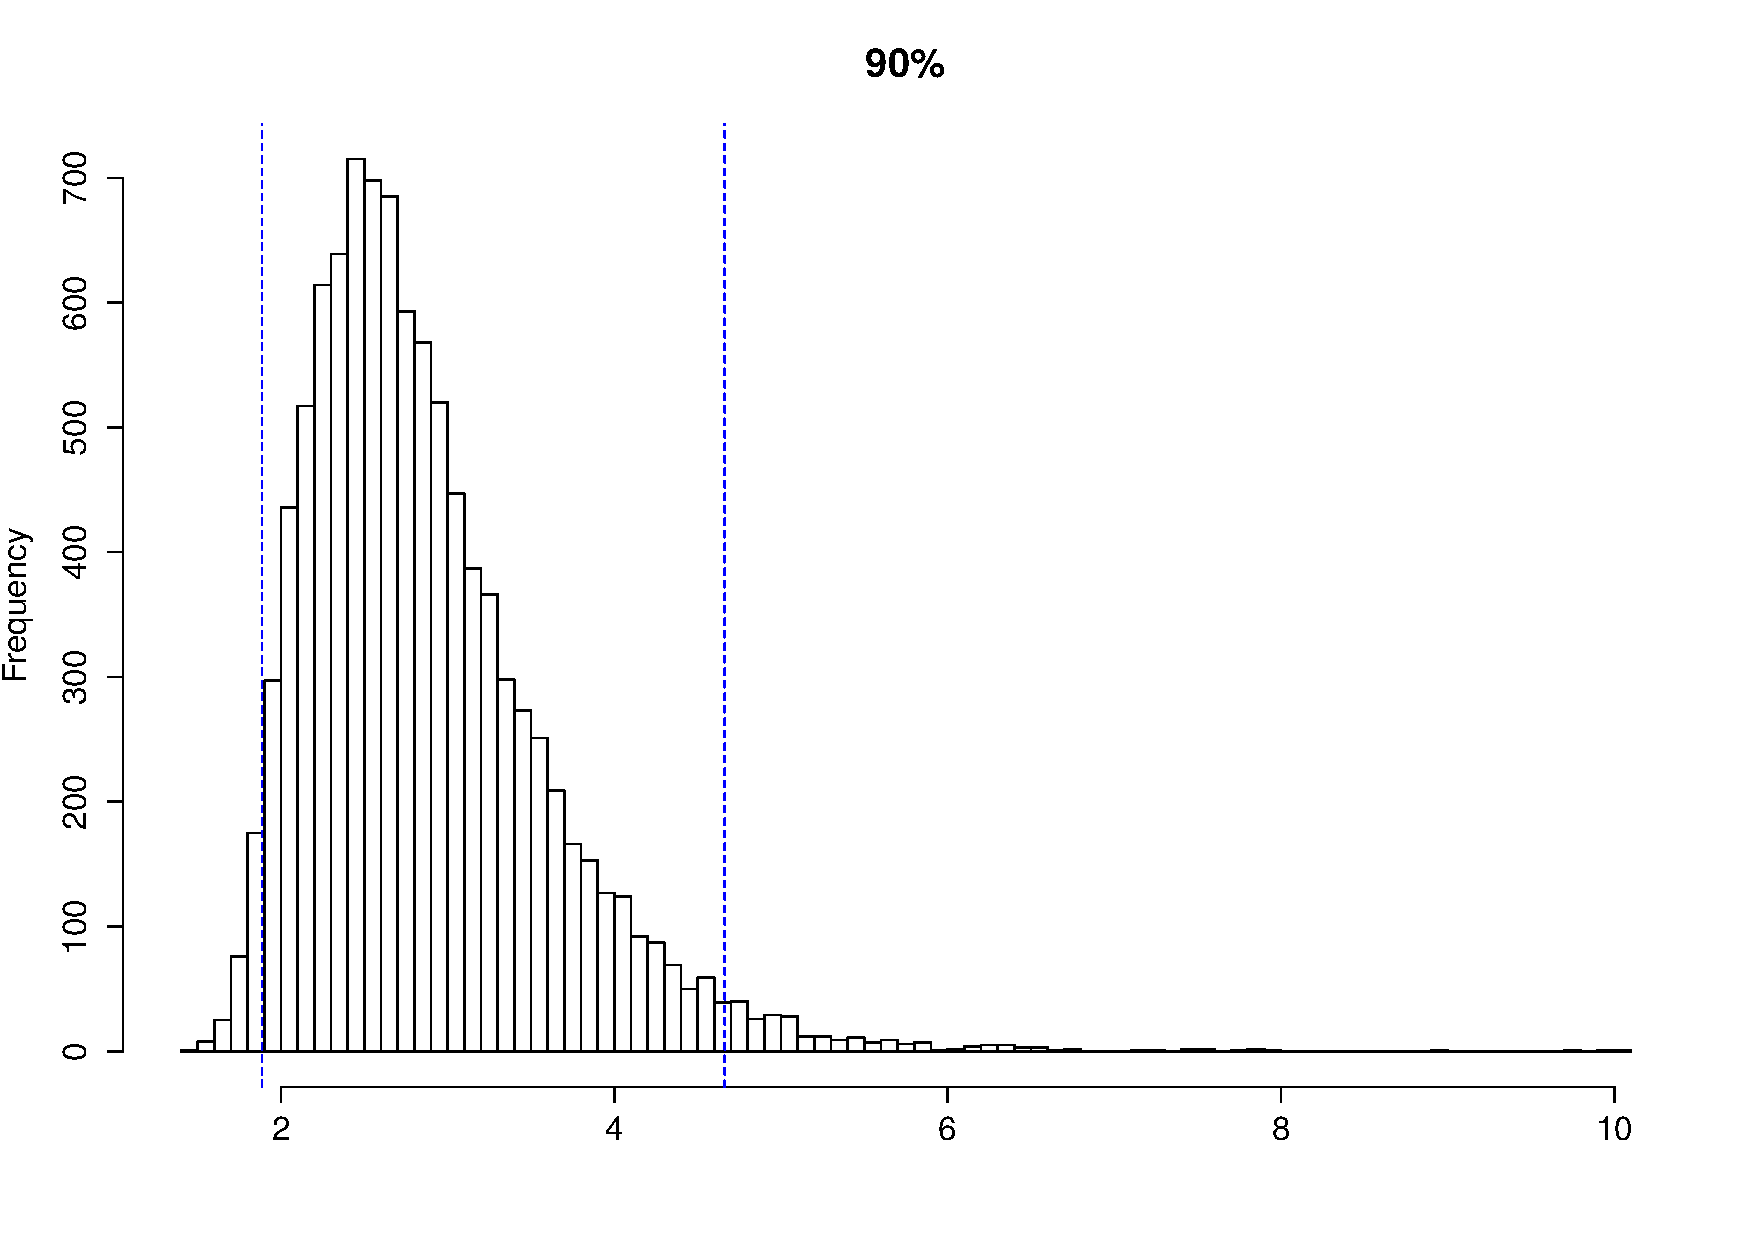
\includegraphics[width = \linewidth]{img/BootstrapParamEMV-90-100.pdf}
        \caption{Quantile à 90\%}
        \label{fig:BPEMV90b}
    \end{subfigure}%
    \begin{subfigure}[t]{0.3\textwidth}
        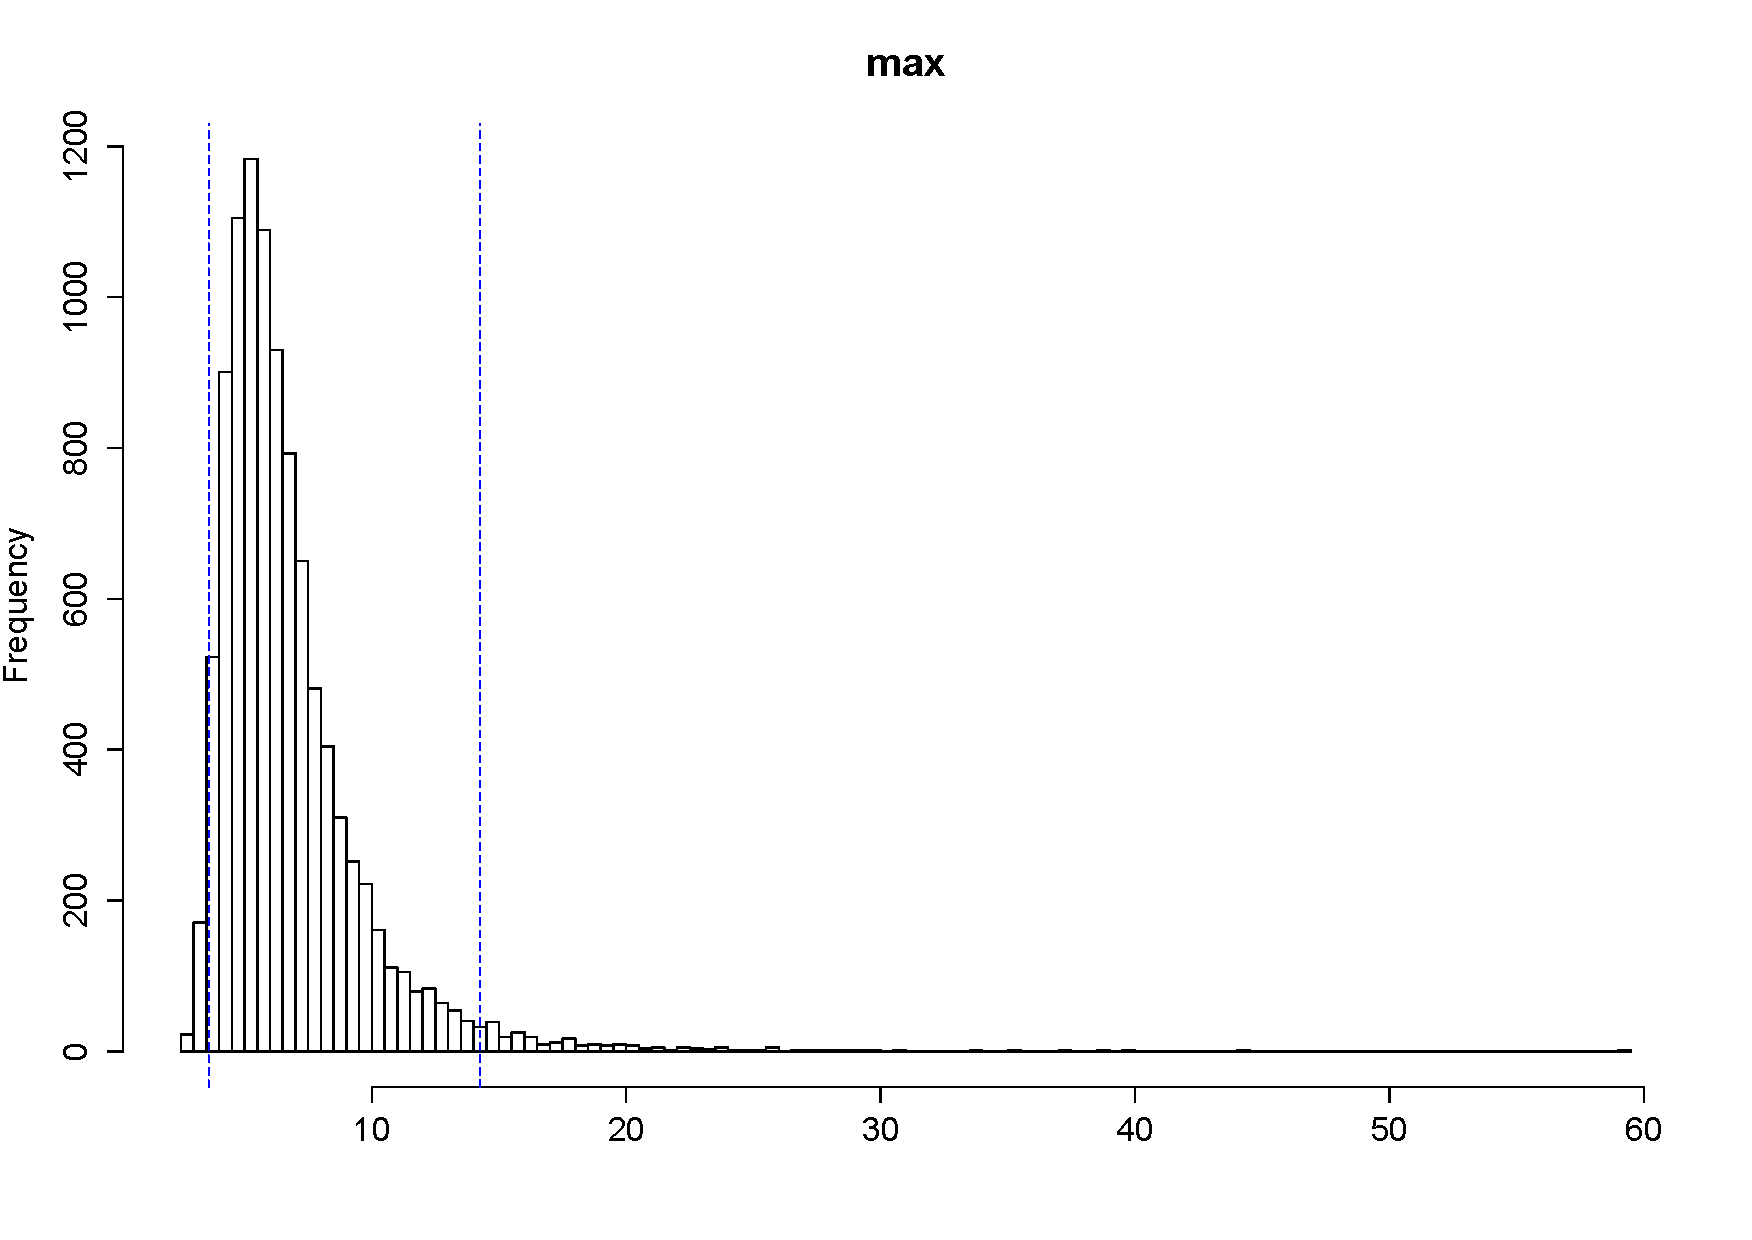
\includegraphics[width = \linewidth]{img/BootstrapParamEMV-Max-100.pdf}
        \caption{Quantile à 99/100 : maximum empirique}
        \label{fig:BPEMVMaxb}
    \end{subfigure}%
    \caption{Histogramme de la distribution du quantile empirique pour n = 100, obtenu par bootstrap paramétrique}
    \label{fig:BPEMVb}
\end{figure}


\subsection{Estimateur de Hill : plus robuste à la spécification}

L'estimateur de Hill consiste à ajuster une loi de Pareto tronquée sur les $k-1$ plus grandes valeurs de l'échantillon, où $k \leq n$. Plus précisément, en notant $X_{(1)},..,X_{(k)}$ les $k$ plus grandes valeurs de l'échantillon $X^{(n)}$, on suppose que :
\[ X_{(1)},..,X_{(k-1)} \sim Pareto(\beta,c=X_{(k)}) \]

Cette hypothèse est plus faible que celle qui affirme que $X$ suit une loi de Pareto de manière globale, utilisée jusqu'ici dans cette partie. Pour $n$ grand $k = o(n)$, on peut l'appliquer à une large classe de lois de probabilité (dites du domaine de Fréchet) dont la queue est similaire à celle d'une loi de Pareto [\cite{Planchet}]\\ 

L'estimateur de Hill est alors l'estimateur du maximum de vraisemblance de ce modèle :
\[ \frac{1}{\widehat{\beta}_{k,H}(X)} = \frac{1}{\widehat{\beta}_{MV}(X_{(1)},..,X_{(k-1)})} = \frac{1}{n} \sum_{j=1}^{k-1}\log \frac{X_{(j)}}{X_{(k)}} \]

Du paramètre estimé par la méthode de Hill, on peut déduire l'estimateur suivant des quantiles suffisament élevés, également appelé estimateur de Hill [\cite{Planchet}] :
\[ \forall\ q > 1-\frac{k}{n},\ \widehat{Q(q)}_{k,H} = X_{(k)} + \left( \frac{n}{k}(1-q) \right)^{-\frac{1}{\widehat{\beta}_{k,H}}} \]
Cet estimateur est convergent si $X$ suit une loi de Pareto dès lors que $k\rightarrow \infty$ et $n\rightarrow \infty$, mais aussi pour toute distribution du domaine de Fréchet si on a de plus $k = o(n)$. Pour satisfaire la condition $q > 1-\frac{k}{n}$, il est nécessaire que $q$ tende vers $1$ quand $n\rightarrow \infty$, par exemple $q = 1-\frac{1}{n}$ dont le quantile $Q(1-\frac{1}{n})$ est l'espérance asymptotique du maximum d'un échantillon de taille $n$. 

\begin{table}[H]
\centering
\begin{tabular}{c|c|ccccc}
&Quantile Théorique&IC Oracle&IC Matthieu avec Beta hat EMV&IC Matthieu avec Beta hat Hill&IC EMV&IC Hill\\
75\%&2&\begin{tabular}{c}$1.76$\\{\small $[ 1.61 , 1.91 ]$ } \end{tabular}&\begin{tabular}{c}$1.94$\\{\small $[ 1.88 , 2 ]$ } \end{tabular}&\begin{tabular}{c}$1.94$\\{\small $[ 1.87 , 2 ]$ } \end{tabular}&\begin{tabular}{c}$1.93$\\{\small $[ 1.56 , 2.46 ]$ } \end{tabular}&\begin{tabular}{c}$2.84$\\{\small $[ 2.76 , 2.96 ]$ } \end{tabular}\\
90\%&3.16&\begin{tabular}{c}$2.66$\\{\small $[ 2.2 , 3.12 ]$ } \end{tabular}&\begin{tabular}{c}$2.42$\\{\small $[ 2.31 , 2.54 ]$ } \end{tabular}&\begin{tabular}{c}$2.42$\\{\small $[ 2.3 , 2.54 ]$ } \end{tabular}&\begin{tabular}{c}$3$\\{\small $[ 2.09 , 4.46 ]$ } \end{tabular}&\begin{tabular}{c}$3.4$\\{\small $[ 2.91 , 4.21 ]$ } \end{tabular}\\
max& 5.48 & \begin{tabular}{c}$6.57$\\{\small $[ 1.52 , 11.62 ]$ } \end{tabular}&\begin{tabular}{c}$4.18$\\{\small $[ 3.96 , 4.39 ]$ } \end{tabular}&\begin{tabular}{c}$4.18$\\{\small $[ 3.96 , 4.39 ]$ } \end{tabular}&\begin{tabular}{c}$5.13$\\{\small $[ 2.97 , 9.1 ]$ } \end{tabular}&\begin{tabular}{c}$4.52$\\{\small $[ 3.12 , 7.49 ]$ } \end{tabular}
\end{tabular}
\caption{n = 30}
\label{tab:resA30}
\end{table} 

\begin{table}[H]
\centering
\begin{tabular}{c|c|ccccc}
&Quantile Théorique&IC Oracle &IC Matthieu avec Beta hat EMV&IC Matthieu avec Beta hat Hill&IC EMV&IC Hill\\
\hline
75\%&2&\begin{tabular}{c}$1.76$\\{\small $[ 1.61 , 1.91 ]$ } \end{tabular}&\begin{tabular}{c}$1.76$\\{\small $[ 1.73 , 1.79 ]$ } \end{tabular}&\begin{tabular}{c}$1.76$\\{\small $[ 1.73 , 1.79 ]$ } \end{tabular}&\begin{tabular}{c}$1.84$\\{\small $[ 1.66 , 2.05 ]$ } \end{tabular}&\begin{tabular}{c}$2.74$\\{\small $[ 2.7 , 2.79 ]$ } \end{tabular}\\
90\%&3.16&\begin{tabular}{c}$2.66$\\{\small $[ 2.2 , 3.12 ]$ } \end{tabular}&\begin{tabular}{c}$2.66$\\{\small $[ 2.6 , 2.72 ]$ } \end{tabular}&\begin{tabular}{c}$2.66$\\{\small $[ 2.61 , 2.71 ]$ } \end{tabular}&\begin{tabular}{c}$2.76$\\{\small $[ 2.32 , 3.3 ]$ } \end{tabular}&\begin{tabular}{c}$3.23$\\{\small $[ 3 , 3.54 ]$ } \end{tabular}\\
max&10&\begin{tabular}{c}$6.57$\\{\small $[ 1.52 , 11.62 ]$ } \end{tabular}&\begin{tabular}{c}$6.57$\\{\small $[ 6.4 , 6.74 ]$ } \end{tabular}&\begin{tabular}{c}$6.57$\\{\small $[ 6.43 , 6.71 ]$ } \end{tabular}&\begin{tabular}{c}$7.7$\\{\small $[ 5.39 , 10.92 ]$ } \end{tabular}&\begin{tabular}{c}$5.72$\\{\small $[ 4.15 , 8.27 ]$ } \end{tabular}
\end{tabular}
\caption{n = 100}
\label{tab:resA100}
\end{table} 


% Ce serait bien de coder ct estimateur-là si on a le temps car l'estimateur Q = quantile théorique d'une Pareto(betaHill), ça ne sert à rien : moins bon que QEMV si on a globalement une Pareto et pas convergent si on n'a que la queue. De même pour le bootstrap (1 c Hill).
% Je ne sais pas comment on pourrait faire un bootstrap (1 c Hill) utile. 

% http://www.ressources-actuarielles.net/EXT/ISFA/fp-isfa.nsf/0/72EE1310B7EBC2A2C1256FD2002E9C76/$FILE/Seance3-01.pdf?OpenElement  page 30

\begin{figure}[H]
    \centering
    \begin{subfigure}[t]{0.3\textwidth}
        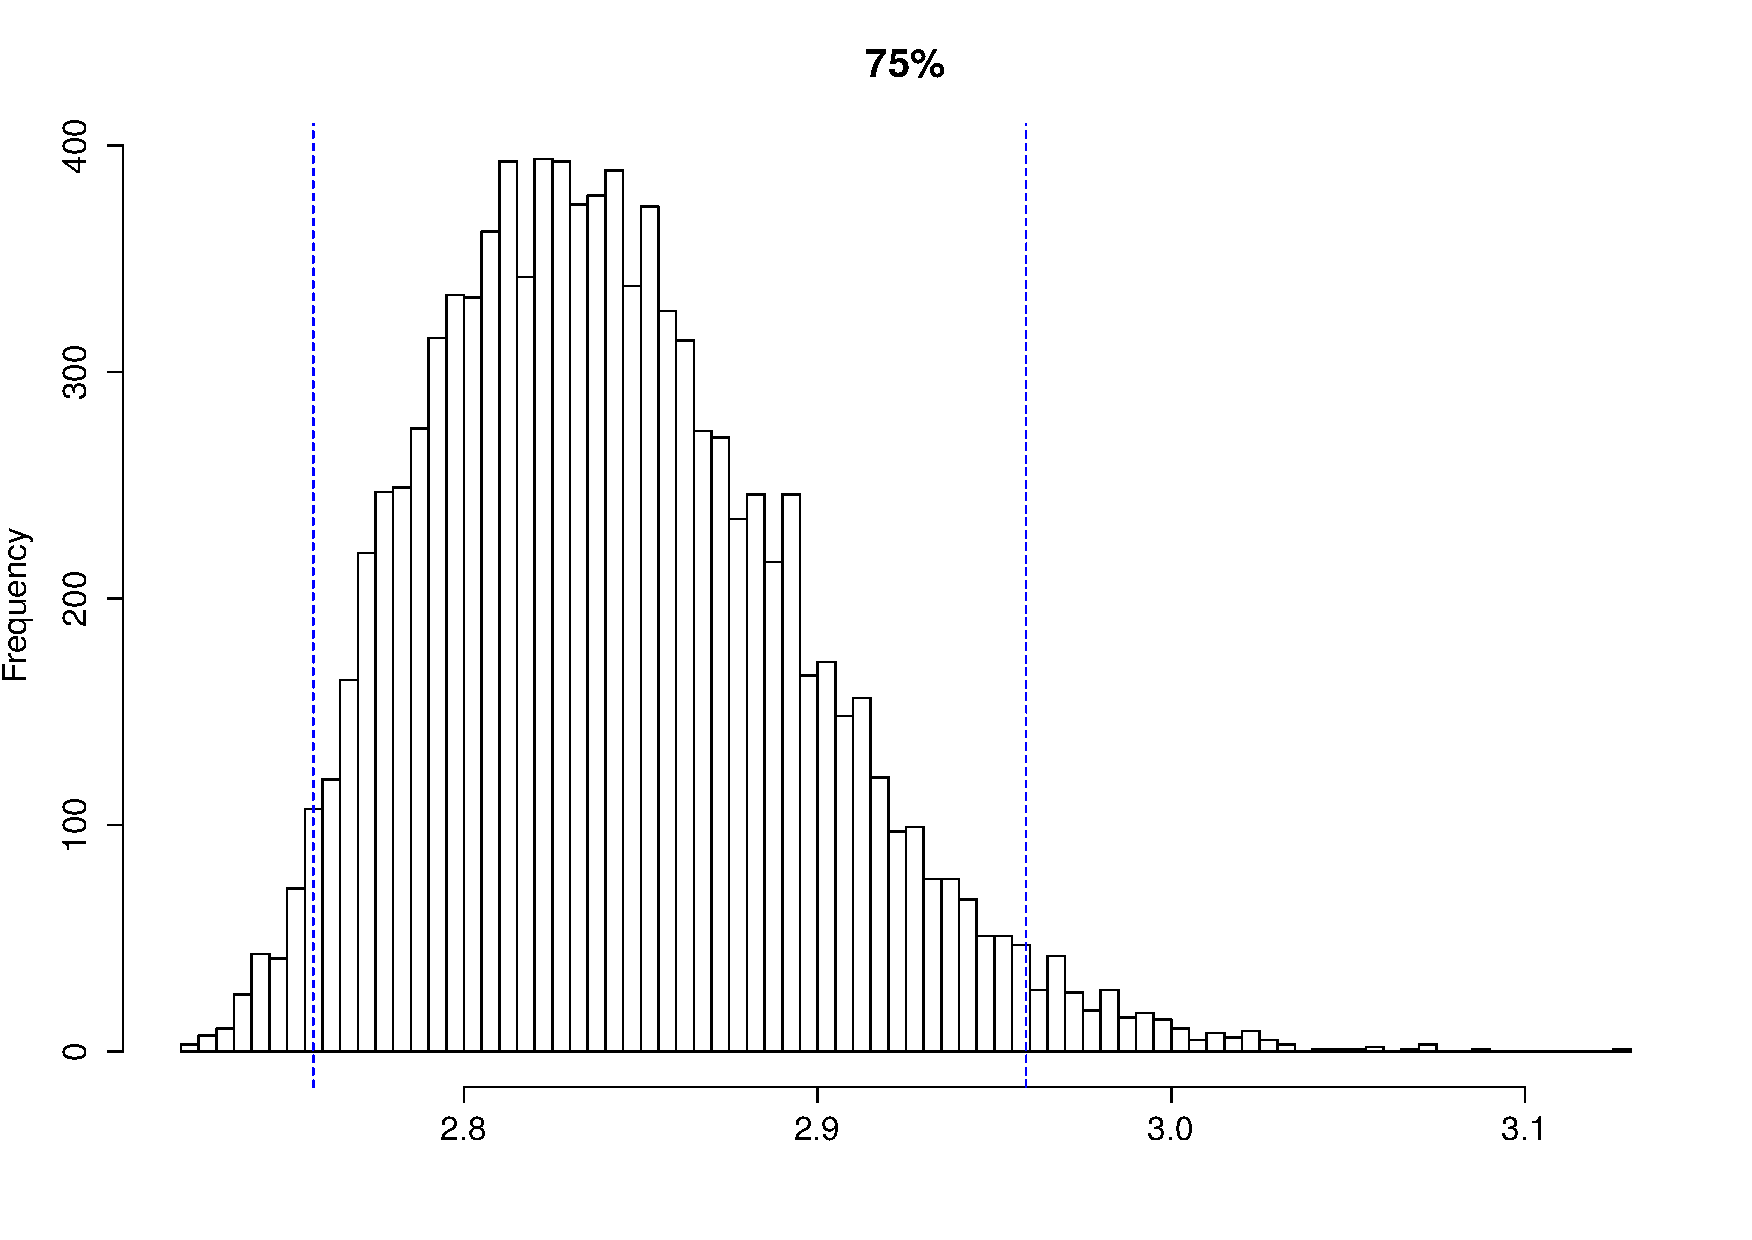
\includegraphics[width = \linewidth]{img/BootstrapAHill-75-30.pdf}
        \caption{Quantile à 75\%}
        \label{fig:BAH75} %BAH : bootstrap 2a hill
    \end{subfigure}%
    \begin{subfigure}[t]{0.3\textwidth}
        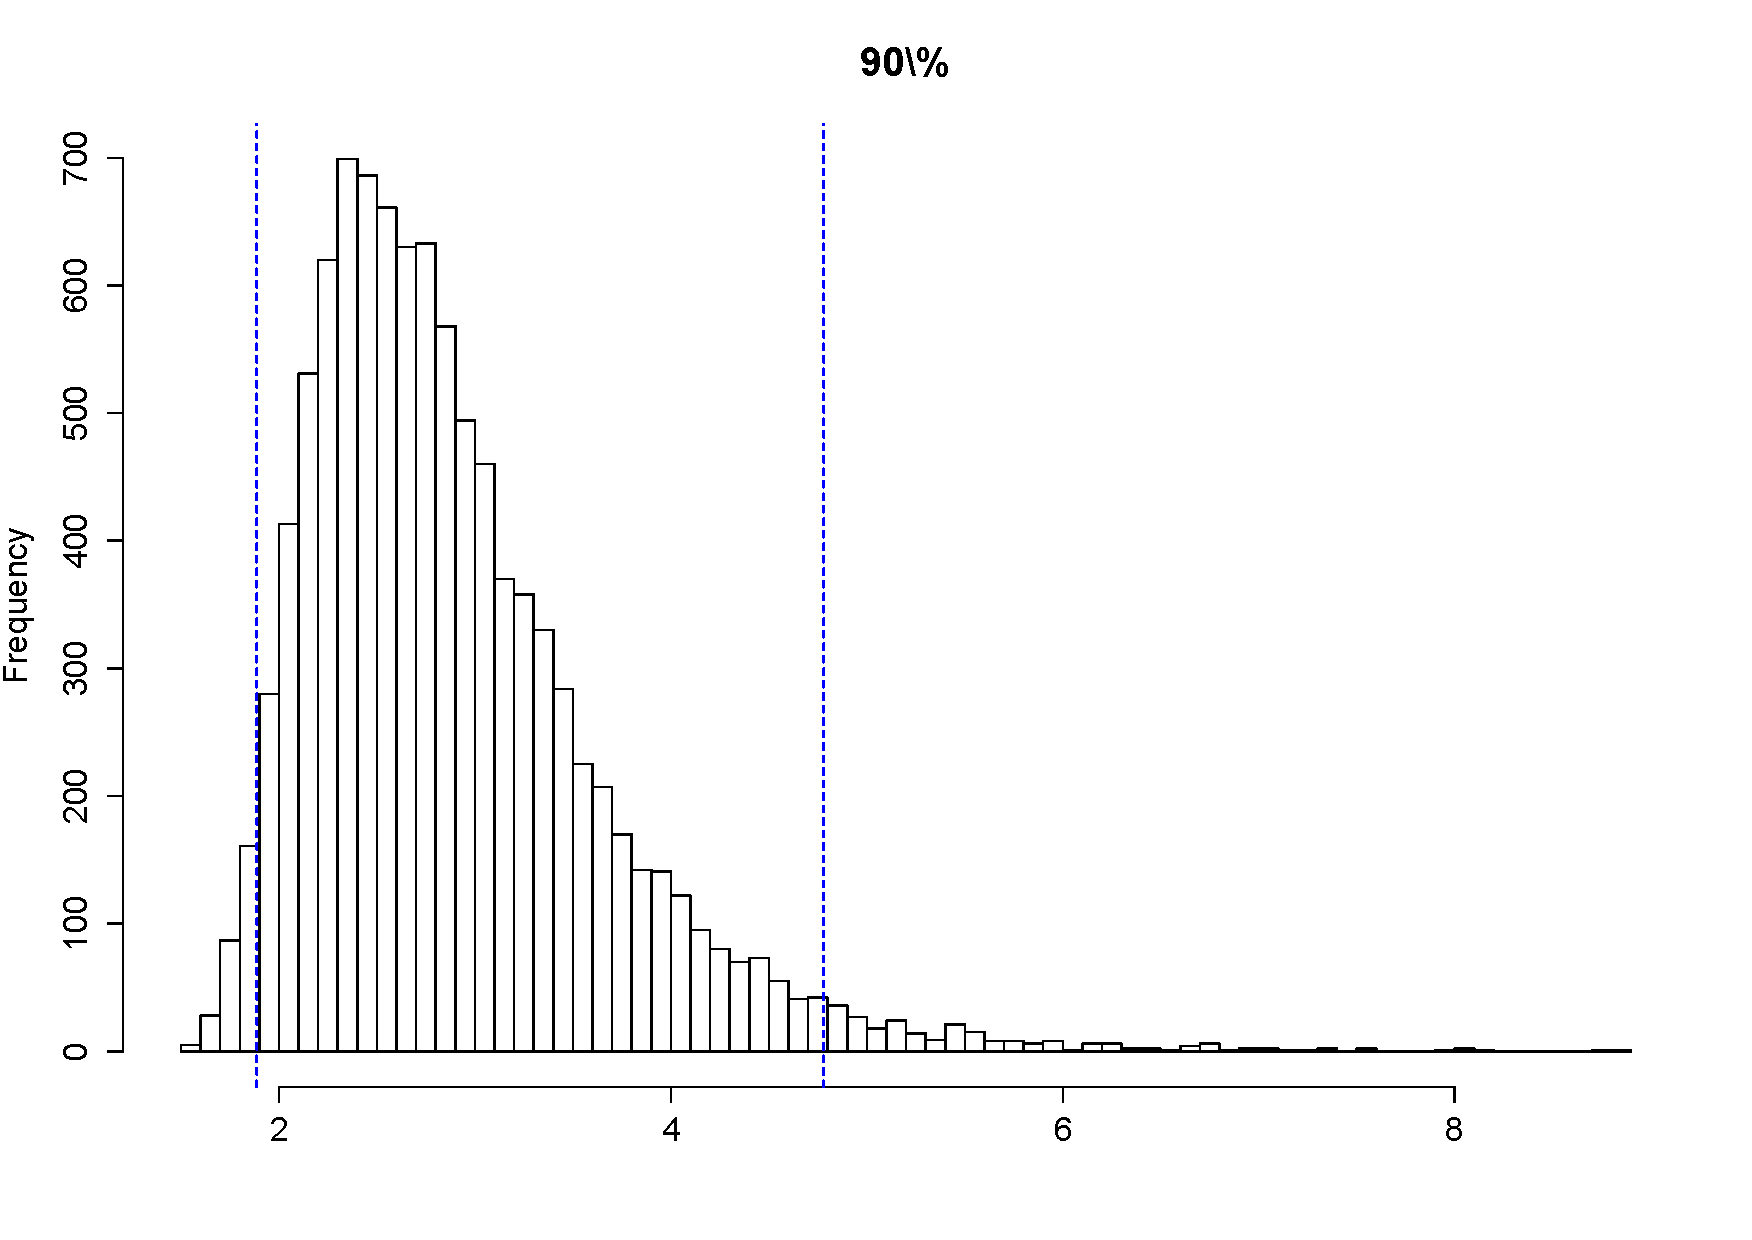
\includegraphics[width = \linewidth]{img/BootstrapAHill-90-30.pdf}
        \caption{Quantile à 90\%}
        \label{fig:BAH90}
    \end{subfigure}%
    \begin{subfigure}[t]{0.3\textwidth}
        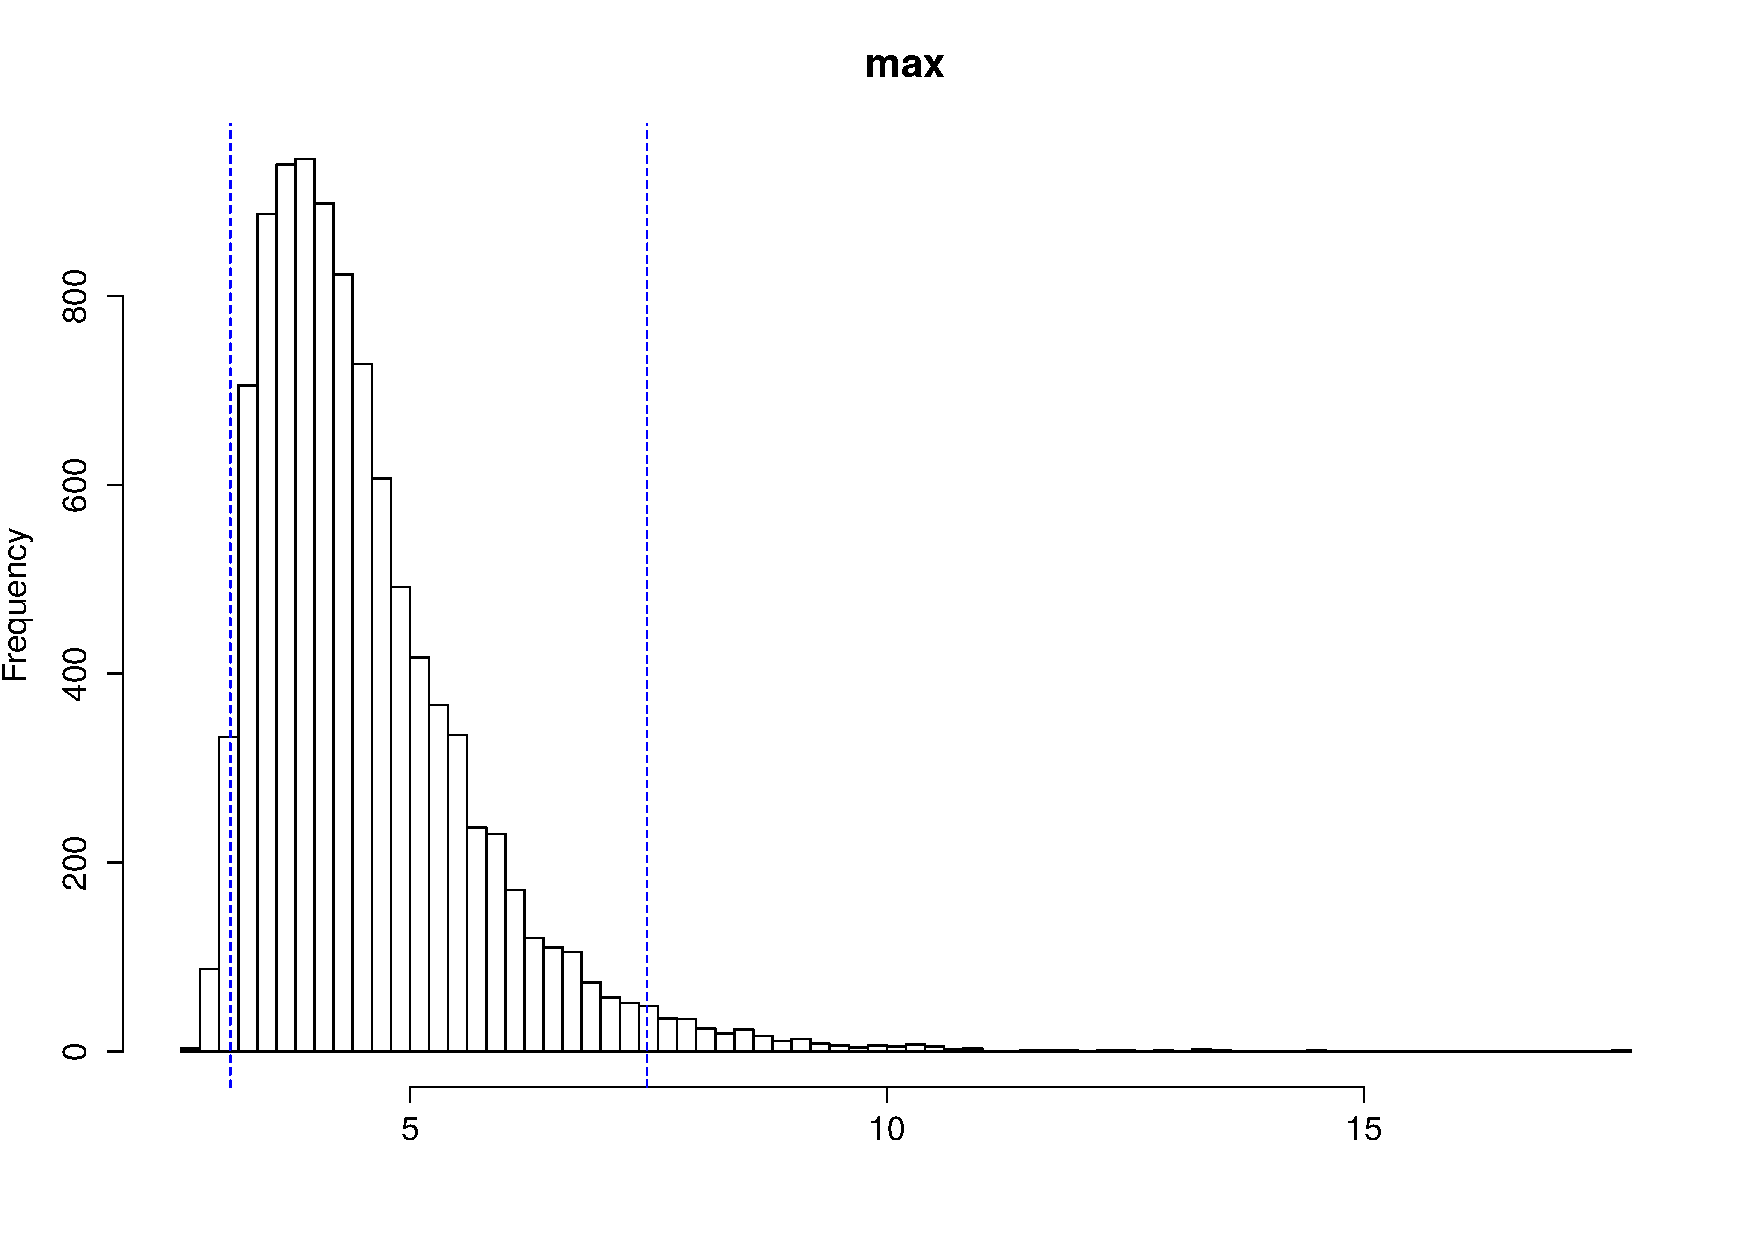
\includegraphics[width = \linewidth]{img/BootstrapAHill-Max-30.pdf}
        \caption{Quantile à 29/30}
        \label{fig:BAHMax}
    \end{subfigure}%
    \caption{Histogramme de la distribution 2a par la méthode de Hill pour n = 30}
    \label{fig:BAH}
\end{figure}

\begin{figure}[H]
    \centering
    \begin{subfigure}[t]{0.3\textwidth}
        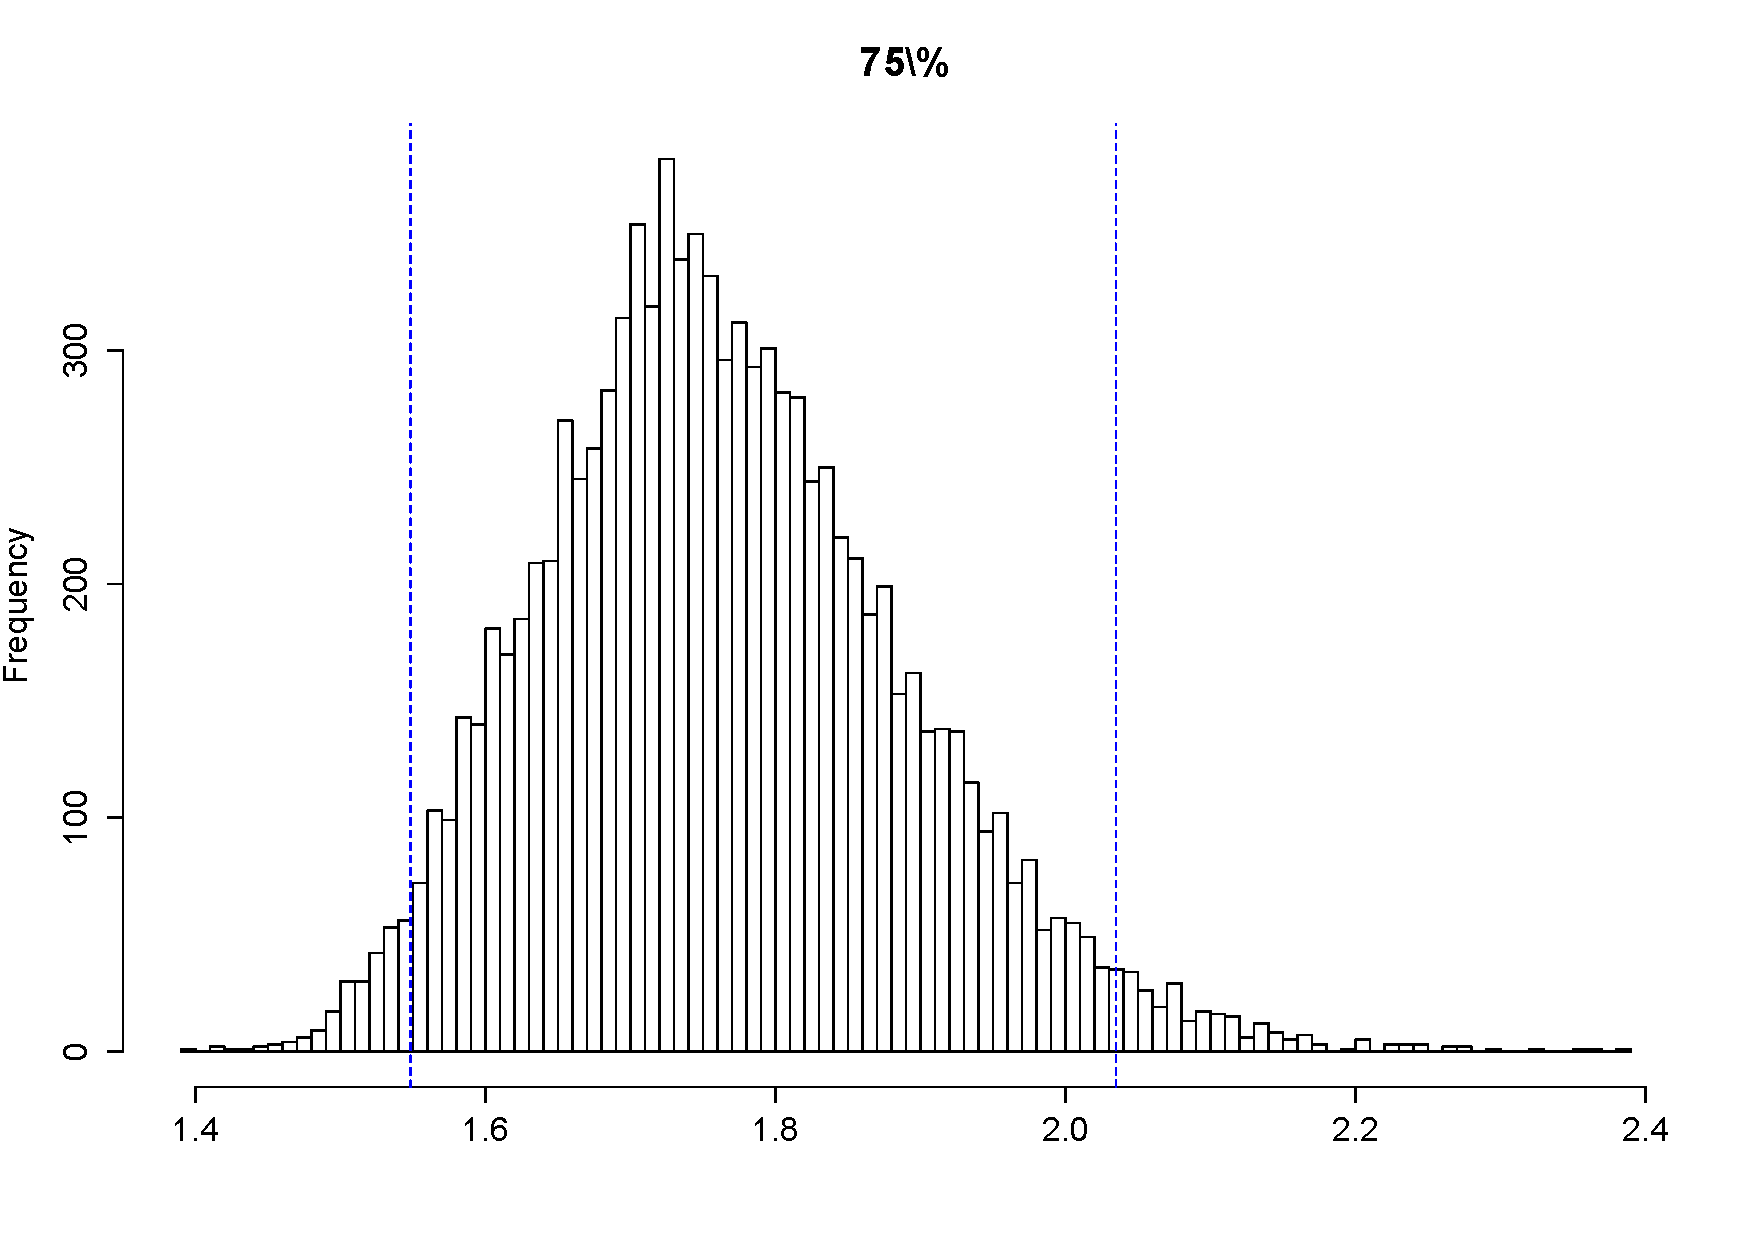
\includegraphics[width = \linewidth]{img/BootstrapParamHill-75-100.pdf}
        \caption{Quantile à 75\%}
        \label{fig:BPH75} %BPH : bootstrap parametrique hill
    \end{subfigure}%
    \begin{subfigure}[t]{0.3\textwidth}
        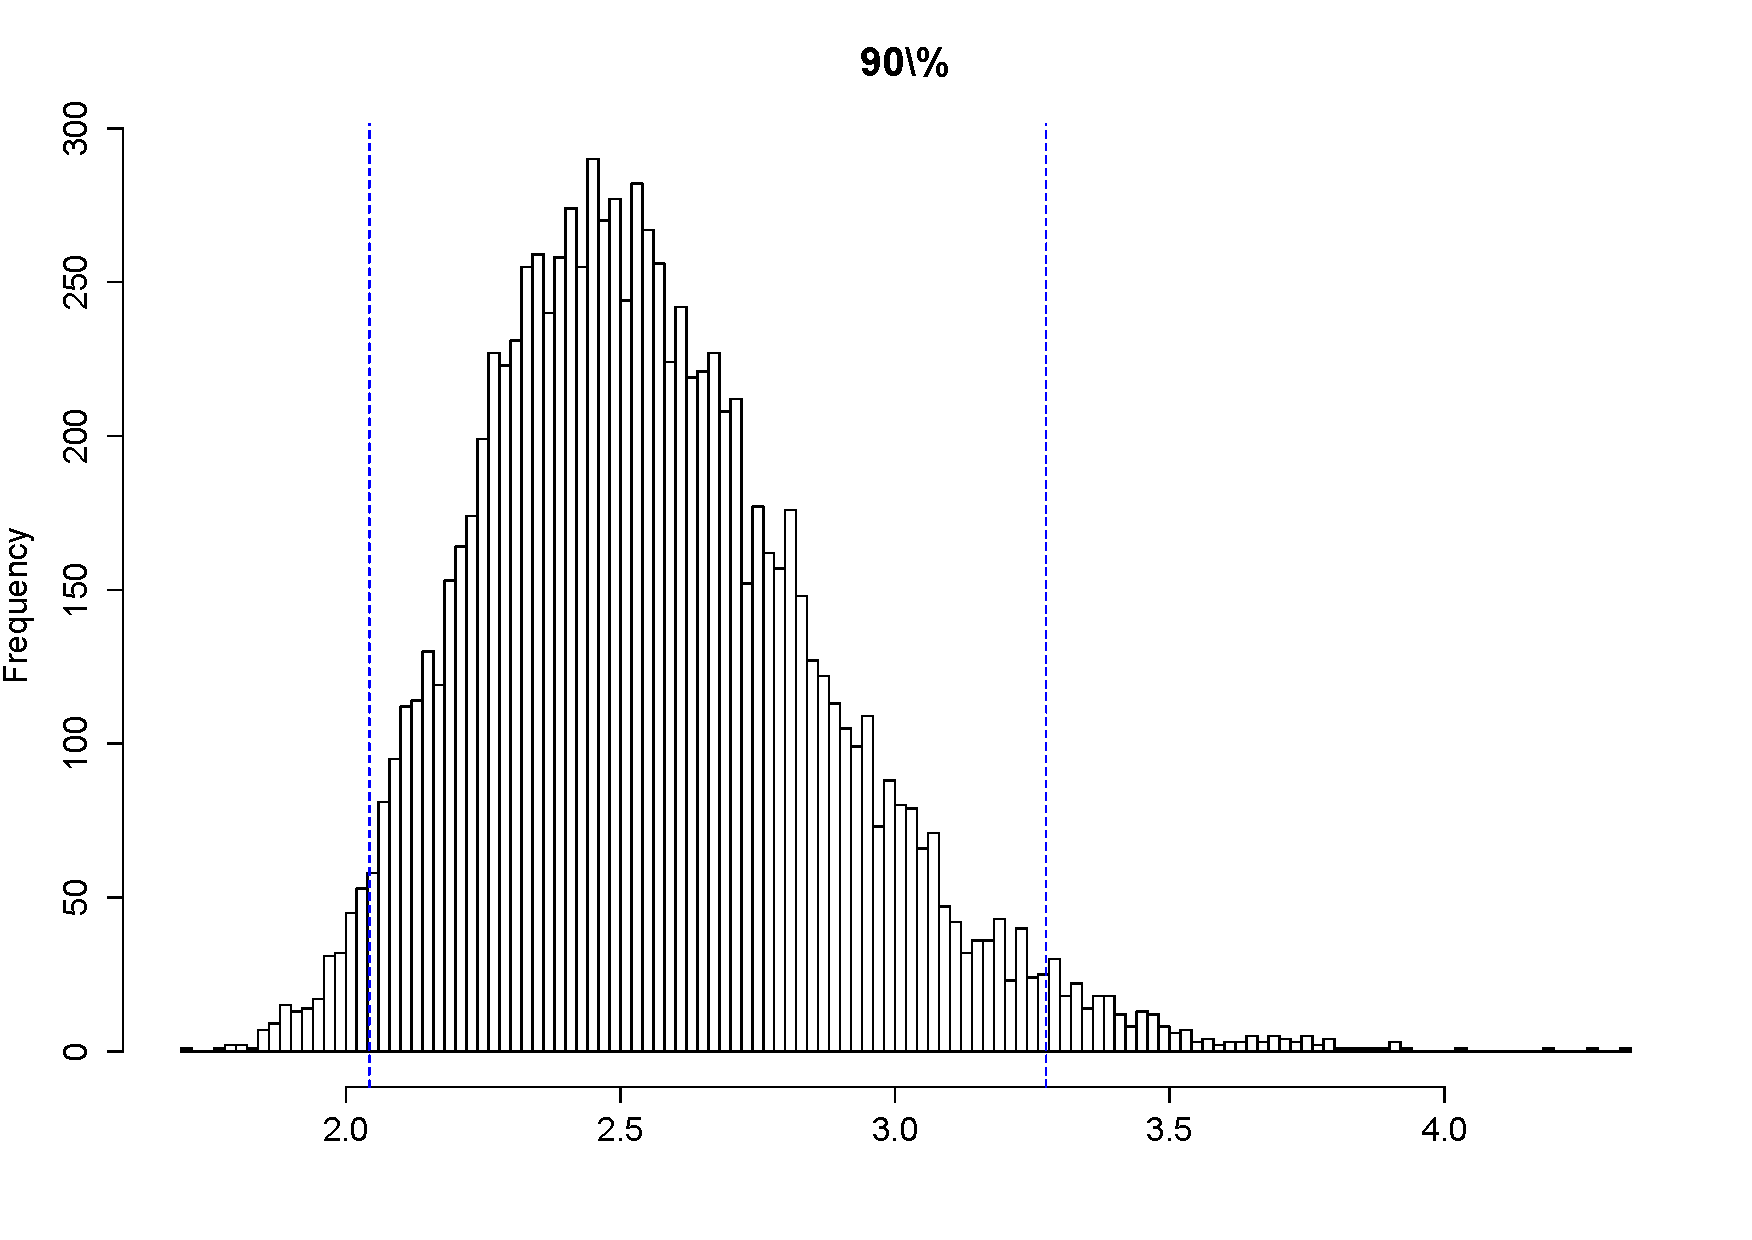
\includegraphics[width = \linewidth]{img/BootstrapParamHill-90-100.pdf}
        \caption{Quantile à 90\%}
        \label{fig:BPH90}
    \end{subfigure}%
    \begin{subfigure}[t]{0.3\textwidth}
        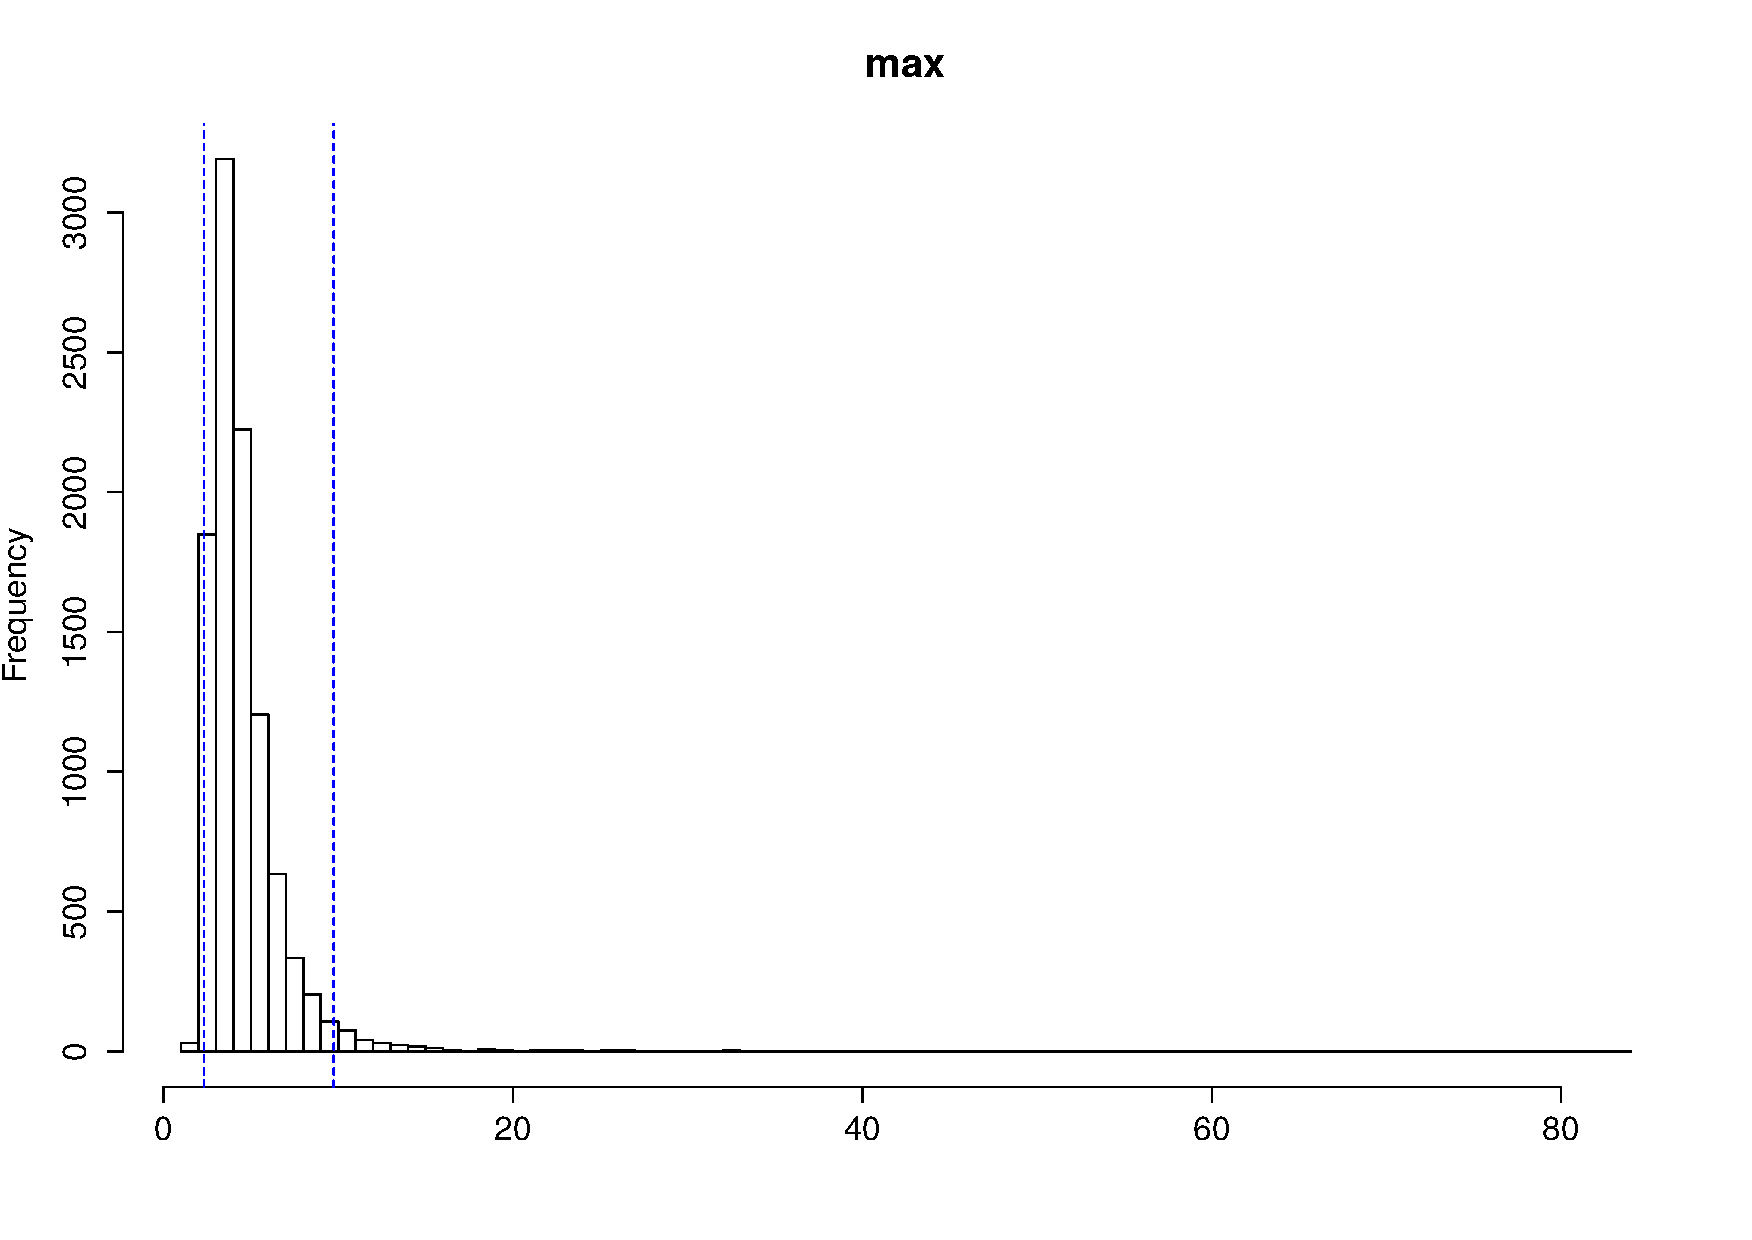
\includegraphics[width = \linewidth]{img/BootstrapParamHill-Max-100.pdf}
        \caption{Quantile à 99/100}
        \label{fig:BPHMax}
    \end{subfigure}%
    \caption{Histogramme de la distribution du Bootstrap paramétrique par la méthode de Hill pour n = 100}
    \label{fig:BPH}
\end{figure}




%%%%%%%%%%%%%%%%%%%%%%%%%%%%%%%%%%%%%%%%%%%%%%%%
%%%%%%%%%%%%%%%%%%%%%%%%%%%%%%%%%%%%%%%%%%%%%%%%


%2c : un calcul de beta0 chapeau avec les donnees, puis simulations de m échantillons de taille n qui suivent cette loi [ pareto(c,beta0 chapeau) ], calcul de m beta chapeau, qui donnent m quantiles en inversant la FdR [avantage : on n'a plus une pareto troncquee comme c'était le cas en 2a] -> inconvenient : on n'a jamais rien vu de tel, et c'est pas mentionné en cours (à vérifier mais je ne crois pas)


\section*{Conclusion}
La méthode standard de bootstrap appliquée à l'estimateur du quantile empirique est d'une efficacité médiocre, qui a cependant pu être améliorée grâce à l'utilisation de méthodes de bootstrap lisse, paramétrique ou non-paramétrique.

\bibliographystyle{plain}
\bibliography{biblio}

\section*{Annexe}
\subsection{Calcul des intervalles de confiance non paramétriques pour les quantiles}
Ces calculs sont inspirés du cours :
\url{http://cermics.enpc.fr/~alfonsi/mrf-quantile.pdf}\\


\section*{Code R}
Le code utilisé est disponible sur \url{https://github.com/BDonnot/Bootstrap}

\end{document}


% Plan de la présentation
% Introduction (Clara)
% I. Non paramétrique :expliquer les IC asymptotiques, expliquer les techniques bootstrap (Clara)
% décrire les résultats (graphes + tableaux) (Benjamin)
% II. Paramétrique : estimer le beta. Deux estimateurs (EMV + hill (robust)) (Matthieu)
% graphes et tableaux (Benjamin)
% Conclusion (Matthieu)

